\documentclass[aspectratio=169]{beamer}

\usetheme{Madrid}
\usecolortheme{default}
\setbeamertemplate{navigation symbols}{}
\setbeamercolor{block title}{bg=blue!70!black,fg=white}
\setbeamercolor{block body}{bg=blue!5,fg=black}
\setbeamercolor{block title alerted}{bg=red!75!black,fg=white}
\setbeamercolor{block body alerted}{bg=red!5,fg=black}
\setbeamercolor{block title example}{bg=green!50!black,fg=white}
\setbeamercolor{block body example}{bg=green!6,fg=black}

\usepackage[utf8]{inputenc}
\usepackage[T1]{fontenc}
\usepackage{amsmath, amssymb, bm, booktabs}
\usepackage{graphicx}
\usepackage{tikz}
\usetikzlibrary{positioning, arrows.meta, shapes.geometric}

\graphicspath{{figures/}}

\title{Low-Rank Architectures and Deep Optimization}
\subtitle{Kernel, mean-field, and feature-learning perspectives}
\author{Janis}
\date{\today}

\begin{document}

\begin{frame}
  \titlepage
\end{frame}

\begin{frame}{Neural networks: scaling laws and depth vs.\ width}
  \small
  \begin{block}{The practical problem}
    \begin{itemize}
      \item We want deep nets to approximate functions or fit data.
      \item \textbf{Optimization} and \textbf{architecture} interact in poorly understood ways.
      \item Classical wisdom: ``go wider and deeper.'' Large-scale evidence refines that.
    \end{itemize}
  \end{block}
  \begin{exampleblock}{Scaling laws (Kaplan et al.\ / OpenAI-style)}
    \begin{itemize}
      \item Test loss often scales as a \textbf{power law} in compute, data, and model size.
      \item With matched compute and data, \textbf{depth and width trade}. Many splits give similar loss if parameters and training budget match.
      \item What matters first is \textbf{scale} (parameters, steps, tokens). Not a unique depth recipe.
      \item Takeaway: need \textbf{structure} (rank, bottlenecks, RF). Not only more MLP layers.
    \end{itemize}
  \end{exampleblock}
\end{frame}

\begin{frame}{Optimization tricks---and what we still do not understand}
  \footnotesize
  \begin{columns}[T]
    \begin{column}{0.52\textwidth}
      \begin{block}{What practitioners use}
        \begin{itemize}
          \item \textbf{SGD} + momentum: damp oscillations. Faster progress when ill-conditioned.
          \item \textbf{Adaptive:} RMSProp, \textbf{Adam} / AdamW. Per-parameter LRs. Often the default.
          \item \textbf{Schedules:} warmup, cosine decay, step decay. Often as important as architecture.
        \end{itemize}
      \end{block}
      \begin{alertblock}{Gap}
        Sharp guarantees for Adam on deep nonconvex losses are limited. Behavior is \textbf{tuned} in practice.
      \end{alertblock}
    \end{column}
    \begin{column}{0.46\textwidth}
      \centering
      \textbf{Adam can look ``unstable''}
      \vspace{0.2em}

      \IfFileExists{figures/ae42c68f73518ebe888dafbcefa117c8abc3ffb6.png}{%
        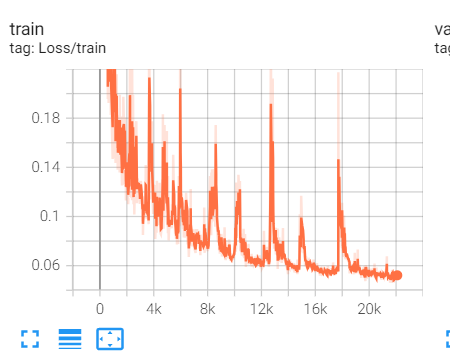
\includegraphics[width=\linewidth,height=0.48\textheight,keepaspectratio]{ae42c68f73518ebe888dafbcefa117c8abc3ffb6.png}%
      }{%
        \fbox{\parbox[c][0.42\textheight][c]{0.92\linewidth}{\centering\scriptsize Add \texttt{figures/ae42c68f73518ebe888dafbcefa117c8abc3ffb6.png}\\(loss vs.\ step: wobbling under Adam)}}%
      }
      \vspace{0.2em}
      \begin{block}{}
        \scriptsize Loss can \textbf{wobble}: sharp oscillations even when the average trend improves. Sensitive to LR, noise, curvature. Motivates \textbf{gentler} landscapes (e.g.\ low-rank RF).
      \end{block}
    \end{column}
  \end{columns}
\end{frame}

\begin{frame}{MMNN (Zhang et al.): low rank + frozen features $\Rightarrow$ very low test error}
  \scriptsize
  \begin{columns}[T]
    \begin{column}{0.52\textwidth}
      \begin{block}{Structured MMNN}
        \begin{itemize}
          \item Each layer: $\bm{h}=\bm{A}\,\sigma(\bm{W}\bm{x}+\bm{b})+\bm{c}$.
          \item \textbf{$\bm{W},\bm{b}$ frozen} (RF). Train \textbf{$\bm{A},\bm{c}$} only. Multi-component rank between layers.
          \item Same param budget as FC. Often \textbf{much smaller} test MSE on oscillatory targets.
        \end{itemize}
      \end{block}
      \begin{exampleblock}{Reported test MSE (SIAM MMNN paper, excerpt)}
        \centering
        \resizebox{\linewidth}{!}{%
        \begin{tabular}{@{}lccc@{}}
          \toprule
          Setting & MMNN (S1) & MMNN (S2) & FCNN \\
          \midrule
          Strategy comp.\ (osc.\ 1D) & $2.0{\times}10^{-5}$ & $4.3{\times}10^{-5}$ & --- \\
          Best MMNN row & $\bm{1.4{\times}10^{-5}}$ & --- & --- \\
          \midrule
          $f_1$ (1D oscillatory) & $2.5{\times}10^{-6}$ & $2.1{\times}10^{-6}$ & $1.7{\times}10^{-4}$ \\
          $f_2$ (2D oscillatory) & $\bm{4.6{\times}10^{-6}}$ & $6.2{\times}10^{-6}$ & $3.3{\times}10^{-5}$ \\
          \bottomrule
        \end{tabular}}
      \end{exampleblock}
    \end{column}
    \begin{column}{0.46\textwidth}
      \centering
      
\includegraphics[width=\linewidth,height=0.38\textheight,keepaspectratio]{four_setups_loss_with_lr_bars.png}
      \vspace{0.2em}
      \begin{alertblock}{Message}
        \scriptsize
        \textbf{Low rank + excellent MSE.} Training $\bm{A}$ is often \textbf{more benign} than full FC at comparable width.
        \textbf{MNIST-class:} RF-LR/MMNN near a wide MLP. \textbf{Far fewer} trainable weights (Zhang et al.).
      \end{alertblock}
    \end{column}
  \end{columns}
\end{frame}

\begin{frame}{Architectural Core: RF-LR / MMNN}
  \begin{columns}[T]
    \begin{column}{0.53\textwidth}
      \begin{block}{Design principle}
        \begin{itemize}
          \item Keep a large random feature bank.
          \item Train only through a small rank-$r$ bottleneck.
          \item Preserve expressive behavior while keeping analysis tractable.
          \item Make channel specialization visible during training.
        \end{itemize}
      \end{block}
    \end{column}
    \begin{column}{0.43\textwidth}
      \centering
      \resizebox{\linewidth}{!}{
      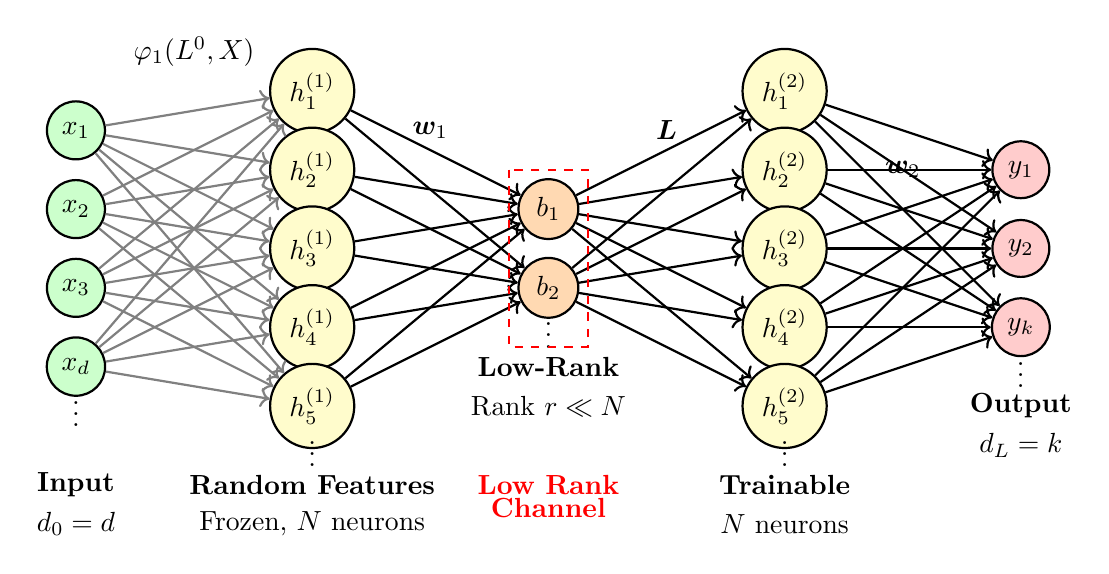
\begin{tikzpicture}[
          node distance=2cm and 3cm,
          neuron/.style={circle, draw, fill=blue!20, minimum size=15pt},
          input/.style={circle, draw, fill=green!20, minimum size=15pt},
          output/.style={circle, draw, fill=red!20, minimum size=15pt},
          hidden/.style={circle, draw, fill=yellow!20, minimum size=15pt},
          bottleneck/.style={circle, draw, fill=orange!30, minimum size=15pt},
          thick
      ]
      
      \node[input] (x1) at (0,2) {$x_1$};
      \node[input] (x2) at (0,1) {$x_2$};
      \node[input] (x3) at (0,0) {$x_3$};
      \node[input] (xd) at (0,-1) {$x_d$};
      \node at (0,-1.5) {$\vdots$};
      
      \node[hidden] (h11) at (3,2.5) {$h_1^{(1)}$};
      \node[hidden] (h12) at (3,1.5) {$h_2^{(1)}$};
      \node[hidden] (h13) at (3,0.5) {$h_3^{(1)}$};
      \node[hidden] (h14) at (3,-0.5) {$h_4^{(1)}$};
      \node[hidden] (h15) at (3,-1.5) {$h_5^{(1)}$};
      \node at (3,-2) {$\vdots$};
      
      \node[bottleneck] (b1) at (6,1) {$b_1$};
      \node[bottleneck] (b2) at (6,0) {$b_2$};
      \node at (6,-0.5) {$\vdots$};
      
      \node[hidden] (h21) at (9,2.5) {$h_1^{(2)}$};
      \node[hidden] (h22) at (9,1.5) {$h_2^{(2)}$};
      \node[hidden] (h23) at (9,0.5) {$h_3^{(2)}$};
      \node[hidden] (h24) at (9,-0.5) {$h_4^{(2)}$};
      \node[hidden] (h25) at (9,-1.5) {$h_5^{(2)}$};
      \node at (9,-2) {$\vdots$};
      
      \node[output] (y1) at (12,1.5) {$y_1$};
      \node[output] (y2) at (12,0.5) {$y_2$};
      \node[output] (yk) at (12,-0.5) {$y_k$};
      \node at (12,-1) {$\vdots$};
      
      \foreach \i in {1,2,3,d} {
          \foreach \j in {11,12,13,14,15} {
              \draw[->, gray] (x\i) -- (h\j);
          }
      }
      
      \foreach \i in {11,12,13,14,15} {
          \foreach \j in {1,2} {
              \draw[->] (h\i) -- (b\j);
          }
      }
      
      \foreach \i in {1,2} {
          \foreach \j in {21,22,23,24,25} {
              \draw[->] (b\i) -- (h\j);
          }
      }
      
      \foreach \i in {21,22,23,24,25} {
          \foreach \j in {1,2,k} {
              \draw[->] (h\i) -- (y\j);
          }
      }
      
      \node at (0,-2.5) {\textbf{Input}};
      \node at (0,-3) {$d_0=d$};
      
      \node at (3,-2.5) {\textbf{Random Features}};
      \node at (3,-3) {Frozen, $N$ neurons};
      
      \node at (6,-1) {\textbf{Low-Rank}};
      \node at (6,-1.5) {Rank $r \ll N$};
      
      \node at (9,-2.5) {\textbf{Trainable}};
      \node at (9,-3) {$N$ neurons};
      
      \node at (12,-1.5) {\textbf{Output}};
      \node at (12,-2) {$d_L=k$};
      
      \node at (1.5,3) {$\varphi_1(L^0,X)$};
      \node at (4.5,2) {$\bm{w}_1$};
      \node at (7.5,2) {$\bm{L}$};
      \node at (10.5,1.5) {$\bm{w}_2$};
      
      \draw[red, thick, dashed] (5.5,1.5) rectangle (6.5,-0.75);
      \node[red] at (6,-2.5) {\textbf{Low Rank}};
      \node[red] at (6,-2.8) {\textbf{Channel}};
      
      \end{tikzpicture}
      }
    \end{column}
  \end{columns}
\end{frame}

\begin{frame}{Main thesis and roadmap}
  \scriptsize
  \begin{block}{From scaling laws, optimizers, and MMNN to this talk}
    \begin{itemize}\setlength{\itemsep}{0.15em}
      \item \textbf{Scaling laws} (Kaplan et al.): matched compute/data $\Rightarrow$ loss tracks scale. Depth/width \textbf{trade}.
      \item We stress \textbf{structure} (rank, frozen RF). It reshapes optimization.
      \item \textbf{Optimization:} SGD/momentum vs.\ Adam. Schedules matter. \textbf{Wobbles} $\Rightarrow$ conditioning and spectra.
      \item \textbf{MMNN} (Zhang et al.): frozen $\bm{W}$, train $\bm{A}$. \textbf{Low test MSE} vs.\ FC. Motivates RF-LR theory.
    \end{itemize}
  \end{block}
  \vspace{-0.2em}
  \begin{columns}[T,onlytextwidth]
    \begin{column}{0.49\textwidth}
      \begin{exampleblock}{Core claim}
        \begin{itemize}\setlength{\itemsep}{0.1em}
          \item Low rank is not only compression.
          \item It isolates optimization-relevant scales.
        \end{itemize}
      \end{exampleblock}
    \end{column}
    \begin{column}{0.49\textwidth}
      \begin{alertblock}{Outcome}
        \begin{itemize}\setlength{\itemsep}{0.1em}
          \item One framework: depth, rank, spectra, features.
          \item NTK and training dynamics together.
        \end{itemize}
      \end{alertblock}
    \end{column}
  \end{columns}
  \vspace{-0.15em}
  \begin{block}{Program}
    \scriptsize
    Theorems: MNIST-style efficiency. Oscillatory regression. Kernel recursions. Step-size stability. Matches MMNN / RF-LR.
  \end{block}
\end{frame}

\begin{frame}[t]{NTK at a glance: settled limit, unfinished business}
  \footnotesize
  \begin{columns}[T,onlytextwidth]
    \begin{column}{0.49\textwidth}
      \begin{block}{Mostly resolved (infinite width)}
        \begin{itemize}\setlength{\itemsep}{0.12em}
          \item Sequential limit $\Rightarrow$ \textbf{lazy training}. Deterministic NTK (Jacot; Chizat).
          \item Explicit recursions. Empirical kernel convergence. Coherent \textbf{kernel picture}.
        \end{itemize}
      \end{block}
      \begin{exampleblock}{Not the full optimization story}
        \begin{itemize}\setlength{\itemsep}{0.12em}
          \item Finite width: feature learning. \textbf{Time-dependent} kernel.
          \item NTK is \textbf{blunt} for end-to-end SGD.
          \item Still useful for the \textbf{initial} curve, conditioning, spectra at large finite width.
        \end{itemize}
      \end{exampleblock}
    \end{column}
    \begin{column}{0.49\textwidth}
      \begin{alertblock}{Large but finite width}
        \scriptsize
        \begin{itemize}\setlength{\itemsep}{0.15em}
          \item \textbf{Feynman diagrams:} Guillen, Misof \& Gerken, \href{https://arxiv.org/abs/2508.11522}{arXiv:2508.11522}.
          \item Systematic \textbf{finite-width} NTK corrections (dNTK/ddNTK). Beyond Gaussian stats.
          \item Recursions for \textbf{early} dynamics.
          \item \textbf{Spectral theory:} Benigni \& Paquette, \href{https://arxiv.org/abs/2508.20036}{arXiv:2508.20036}.
          \item NTK \textbf{eigenvalue distribution}. Quadratic scalings (sample--dimension--width). Near interpolation.
        \end{itemize}
      \end{alertblock}
      \vspace{0.15em}
      \begin{block}{}
        \scriptsize
        \textbf{Takeaway:} refined NTK tools help the \textbf{opening} of training and stability. Before mean-field / feature learning.
      \end{block}
    \end{column}
  \end{columns}
\end{frame}

\begin{frame}{Neural Tangent Kernel (NTK)}
  \small
  \begin{block}{Lazy training and the kernel}
    \begin{itemize}
      \item Infinite-width (sequential) limit: training linearizes.
      \item Optimization governed by a fixed Gram matrix and its spectrum.
      \item RF-LR NTK: explicit layerwise recursion. Visible $1/r$ per bottleneck. Rank at leading order.
    \end{itemize}
  \end{block}
  \begin{exampleblock}{What we read off from the NTK}
    \begin{itemize}
      \item Local convergence. Step-size stability. E.g.\ $\lambda_{\max}$, conditioning of centered kernel.
      \item Depth scaling of correlations. Kernel geometry. Edge-of-chaos alignment across layers.
      \item RKHS comparison: expressivity vs optimization geometry. When class matches shallow ReLU despite low rank.
    \end{itemize}
  \end{exampleblock}
  \begin{alertblock}{High-dimensional and concentration}
    \begin{itemize}
      \item Spherical / equicorrelated data: simpler spectra.
      \item Generic data: often worse conditioning. Geometry matters.
    \end{itemize}
  \end{alertblock}
\end{frame}

\begin{frame}{Mean-field viewpoint}
  \small
  \begin{block}{Beyond a fixed kernel}
    \begin{itemize}
      \item Mean-field: evolving weight distributions as width grows. Measures or particles.
      \item Training need not stay lazy.
      \item Deep RF-LR: tractable limiting flow.
      \item Frozen RF: rich mixing directions. Low-rank readouts train.
    \end{itemize}
  \end{block}
  \begin{exampleblock}{What the mean-field analysis targets}
    \begin{itemize}
      \item Well-posed limiting dynamics. Finite-width error control toward the limit.
      \item \textbf{If} dynamics converge: limit can be a \textbf{global} minimizer of population loss. i.i.d.\ init.
      \item Avoids degenerate collapse from full-rank multilayer mean-field. Under RF-LR constraints.
    \end{itemize}
  \end{exampleblock}
  \begin{alertblock}{Feature learning}
    \begin{itemize}
      \item Specialization. Log-ratio growth. Structured internal features.
      \item Tied to dynamics---not only kernel regression.
    \end{itemize}
  \end{alertblock}
\end{frame}

\begin{frame}{Theorem 1: Infinite-Width NTK Recursion}
  \small
  \begin{block}{Statement}
    \begin{itemize}
      \item Setup: sequential infinite-width limit of the RF-LR NTK.
      \item Object: recursion for the mean kernel across layers.
    \end{itemize}
    \[
    \Theta^{(1)}=1+\Sigma^{(1)}
    \]
    \[
    \Theta^{(\ell)}=1+\frac{1}{r}\Theta^{(\ell-1)}\dot{\Sigma}^{(\ell)}+\frac{1}{r}\Sigma^{(\ell)}
    \]
  \end{block}
  \begin{alertblock}{Interpretation}
    The recursion makes the low-rank contribution explicit.

    Each bottleneck contributes a visible factor $1/r$.

    Rank therefore enters the kernel at leading order.

    This is the basis for the later depth and conditioning results.
  \end{alertblock}
\end{frame}

\begin{frame}{Theorem 2: Depth Scaling of the Proxy Kernel}
  \small
  \begin{block}{Statement}
    \begin{itemize}
      \item Setup: proxy kernel along deep RF-LR layers.
      \item Object: correlation alignment and diagonal-off-diagonal gap.
    \end{itemize}
    \[
    1-\rho_k=\Theta(k^{-2})
    \]
    \[
    \Theta_{\mathrm{diag}}^{(k)}-\Theta_{\mathrm{off}}^{(k)}
    =\Theta\!\left(\frac{1}{rk}\right)
    \]
  \end{block}
  \begin{alertblock}{Interpretation}
    Depth drives the proxy kernel toward a nearly constant regime.

    The informative gap decays at rate $1/(rk)$.

    Rank moderates, but does not remove, this collapse.

    The theorem quantifies the depth-rank tradeoff in the kernel regime.
  \end{alertblock}
\end{frame}

\begin{frame}{Theorem 3: Conditioning Regimes}
  \small
  \begin{block}{Statement}
    \begin{itemize}
      \item Setup: condition number of the centered RF-LR kernel.
      \item Compare generic data with equicorrelated and spherical regimes.
    \end{itemize}
    \[
    \kappa \ge \Omega(rL)
    \]
    \[
    \kappa_{\perp}=1,\qquad \kappa_{\perp}=1+o(1)
    \]
  \end{block}
  \begin{alertblock}{Interpretation}
    In generic geometries, conditioning worsens with depth and rank.

    Equicorrelated and spherical regimes remain well conditioned.

    The optimization picture is therefore geometry-dependent.

    Architecture alone does not determine conditioning.
  \end{alertblock}
\end{frame}

\begin{frame}{Kernel-Regime Summary}
  \scriptsize
  \begin{block}{Comparison table}
    \centering
    \begin{tabular}{@{}p{0.18\linewidth}p{0.34\linewidth}p{0.40\linewidth}@{}}
      \toprule
      & \textbf{Fully trained nets} & \textbf{RF-LR / MMNN} \\
      \midrule
      Trainable & all layers & readouts, biases \\
      Scaling & depth and EOC & depth and rank \\
      Kernel size & can grow & saturates \\
      Centered gap & correlation driven & $\asymp 1/(rL)$ \\
      \bottomrule
    \end{tabular}
  \end{block}
  \begin{alertblock}{Message}
    The optimization question is the same in both settings.

    The RF-LR model makes the relevant scales explicit.

    Depth, rank, and conditioning can be tracked directly.

    This is why it is useful as a reference model.
  \end{alertblock}
\end{frame}

\begin{frame}{Theorem 4: Low Rank Is Enough for the RKHS}
  \small
  \begin{block}{Statement}
    \begin{itemize}
      \item Setup: three-layer mean RF-LR kernel with isotropic random features.
      \item Randomness changes coefficients, but not the endpoint exponent.
      \item Claim: the induced RKHS equals the shallow ReLU RKHS.
    \end{itemize}
    \[
    \mathcal{H}_{\mathrm{RF\text{-}LR}}=\mathcal{H}_{\mathrm{ReLU}}
    \]
  \end{block}
  \begin{alertblock}{Interpretation}
    The random low-rank bottleneck does not change the RKHS exponent.

    It modifies the coefficient, not the functional class.

    The gain therefore does not come from a larger RKHS.

    It comes from conditioning, spectra, and training geometry.
  \end{alertblock}
\end{frame}

\begin{frame}{Theorem 5: Mean-Field Well-Posedness and Global Minimizers}
  \small
  \begin{block}{Statement}
    \begin{itemize}
      \item Setup: mean-field dynamics for deep RF-LR training.
      \item The mean-field flow is well posed.
      \item If the dynamics converges, the limit is globally optimal.
    \end{itemize}
  \end{block}
  \begin{alertblock}{Interpretation}
    The result holds under standard i.i.d. initialization.

    Frozen random features preserve the required richness across depth.

    This avoids the collapse mechanism present in full-rank multilayer theory.

    It provides the dynamic counterpart to the kernel results.
  \end{alertblock}
\end{frame}

\begin{frame}{Theorem 6: Log-Ratio Growth and Channel Dominance}
  \small
  \begin{block}{Statement}
    \begin{itemize}
      \item Setup: compare two channels at a fixed point $x_0$.
      \item Observable: the log-ratio $R_{12}(t,x_0)$.
    \end{itemize}
    \[
    \partial_t R_{12}(t,x_0)\ge 0
    \]
  \end{block}
  \begin{alertblock}{Interpretation}
    Log-ratios quantify channel dominance at a fixed location.

    Positive growth implies persistence and amplification of dominance.

    The specialization mechanism is therefore dynamical, not only visual.

    This gives a rigorous entry point into feature learning.
  \end{alertblock}
\end{frame}

\begin{frame}{Main Contributions}
  \begin{block}{Theory}
    \begin{itemize}
      \item Explicit scaling laws. Not only heuristic depth--rank talk.
      \item Weaker assumptions than earlier drafts.
    \end{itemize}
  \end{block}
  \begin{alertblock}{Diagnostics}
    \begin{itemize}
      \item Expressivity split from conditioning and optimization.
      \item Observables for feature learning: log-ratios, partials, symmetry.
    \end{itemize}
  \end{alertblock}
\end{frame}

\begin{frame}{Depth and Rank in Kernel Geometry}
  \begin{columns}[T]
    \begin{column}{0.49\textwidth}
      
\includegraphics[width=\linewidth]{confirm_thm15.png}
    \end{column}
    \begin{column}{0.49\textwidth}
      
\includegraphics[width=\linewidth]{one_minus_rho_vs_depth_loglog.png}
    \end{column}
  \end{columns}
  \vspace{0.4em}
  \begin{itemize}
    \item The empirical curves follow the predicted scaling law.
    \item Correlations align across depth.
    \item Depth flattens the kernel geometry.
    \item Rank controls the decay of the informative gap.
  \end{itemize}
\end{frame}

\begin{frame}{Further Evidence for Depth Scaling}
  \small
  \begin{columns}[T]
    \begin{column}{0.49\textwidth}
      
\includegraphics[width=\linewidth,height=0.29\textheight,keepaspectratio]{confirm_prop17.png}
    \end{column}
    \begin{column}{0.49\textwidth}
      
\includegraphics[width=\linewidth,height=0.29\textheight,keepaspectratio]{decay_vs_depth.png}
    \end{column}
  \end{columns}
  \vspace{0.35em}
  \begin{columns}[T]
    \begin{column}{0.49\textwidth}
      
\includegraphics[width=\linewidth,height=0.29\textheight,keepaspectratio]{variance_vs_r.png}
    \end{column}
    \begin{column}{0.49\textwidth}
      
\includegraphics[width=\linewidth,height=0.29\textheight,keepaspectratio]{min_eig_mean_vs_r.png}
    \end{column}
  \end{columns}
  \vspace{0.3em}
  \begin{itemize}
    \item Four observables support the same scaling law.
    \item Gap decay, variance decay, and spectral behavior are consistent.
    \item Finite-rank corrections remain visible numerically.
    \item The agreement is not confined to a single statistic.
  \end{itemize}
\end{frame}

\begin{frame}{Conditioning Is the Optimization Bottleneck}
  \begin{columns}[T]
    \begin{column}{0.49\textwidth}
      
\includegraphics[width=\linewidth]{condition_number_proxy_vs_empirical.png}
    \end{column}
    \begin{column}{0.49\textwidth}
      
\includegraphics[width=\linewidth]{condition_number_highdim_spherical.png}
    \end{column}
  \end{columns}
  \vspace{0.4em}
  \begin{itemize}
    \item The deterministic proxy tracks the empirical condition number well.
    \item Data geometry drives the conditioning behavior.
    \item Benign regimes remain stable across depth.
    \item Poorly conditioned regimes deteriorate quickly.
  \end{itemize}
\end{frame}

\begin{frame}{Smallest Eigenvalue and Difficult Regimes}
  \begin{columns}[T]
    \begin{column}{0.49\textwidth}
      
\includegraphics[width=\linewidth,height=0.33\textheight,keepaspectratio]{min_eig_distribution.png}
    \end{column}
    \begin{column}{0.49\textwidth}
      
\includegraphics[width=\linewidth,height=0.33\textheight,keepaspectratio]{condition_number_non_equicorrelated.png}
    \end{column}
  \end{columns}
  \vspace{0.4em}
  \begin{itemize}
    \item The lower edge of the spectrum controls the hardest cases.
    \item Small eigenvalues slow convergence and reduce stability.
    \item The histogram makes this concentration visible.
    \item Low rank does not erase difficult geometry.
  \end{itemize}
\end{frame}

\begin{frame}{Rank Helps, But Not Uniformly}
  \begin{columns}[T]
    \begin{column}{0.49\textwidth}
      
\includegraphics[width=\linewidth]{condition_number_non_equicorrelated.png}
    \end{column}
    \begin{column}{0.49\textwidth}
      
\includegraphics[width=\linewidth]{kernel_regression_risk_vs_r.png}
    \end{column}
  \end{columns}
  \vspace{0.4em}
  \begin{itemize}
    \item Low rank is not a universal remedy.
    \item Hard non-equicorrelated data may remain poorly conditioned.
    \item The gain is quantitative rather than absolute.
    \item Rank provides a controllable tradeoff.
  \end{itemize}
\end{frame}

\begin{frame}{Expressivity Is Not the Whole Story}
  \begin{columns}[T]
    \begin{column}{0.54\textwidth}
      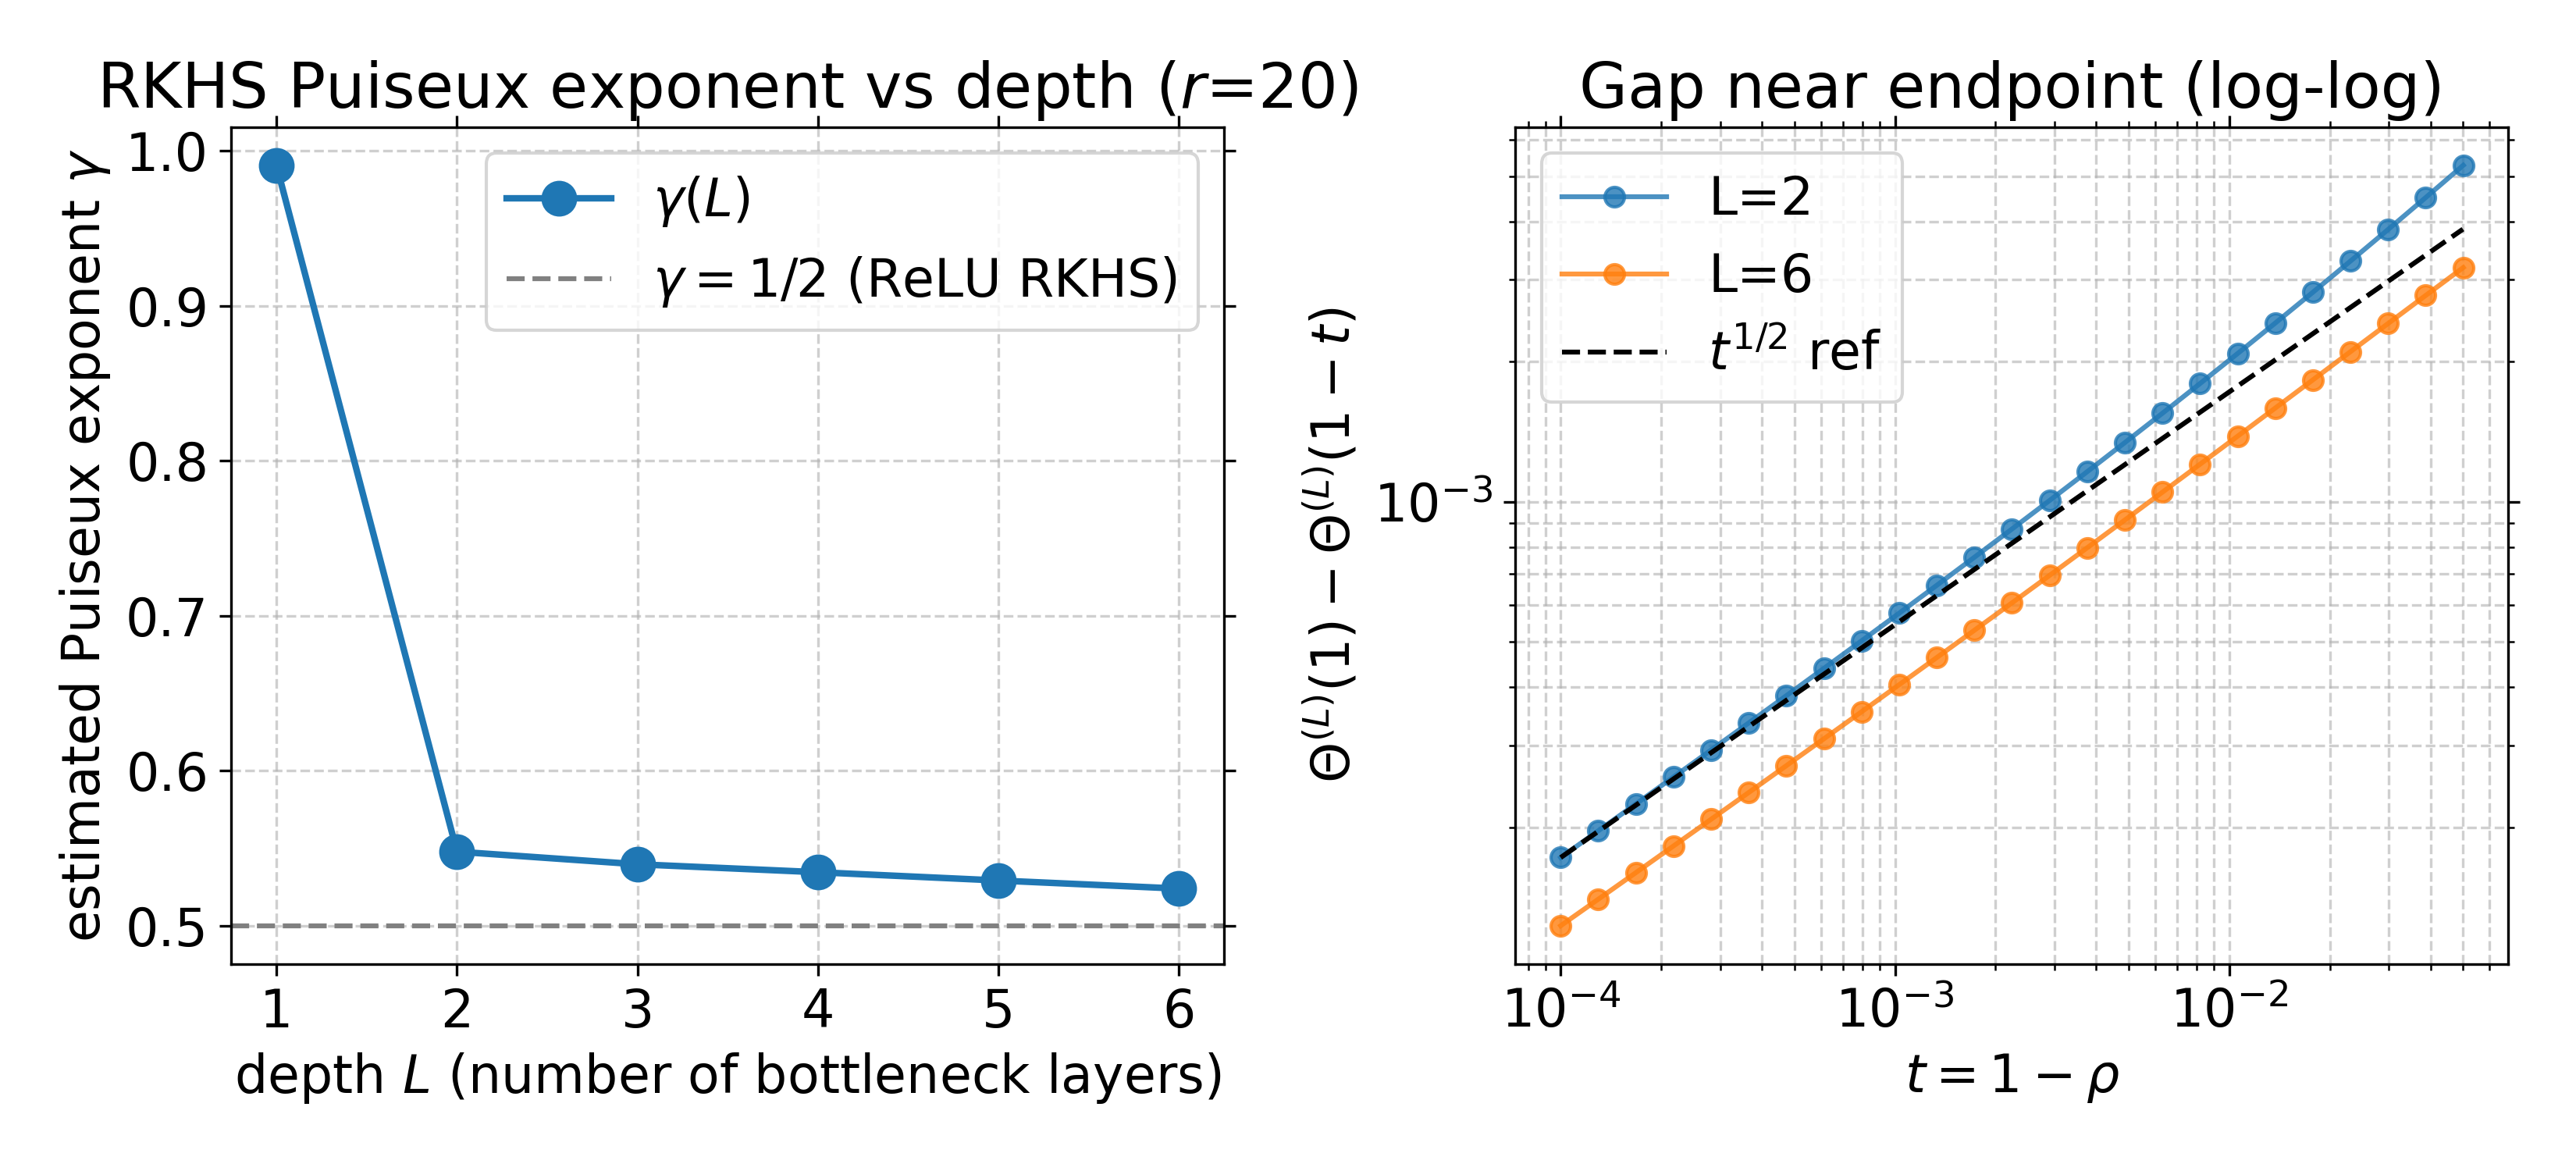
\includegraphics[width=\linewidth]{rkhs_puiseux_exponent_vs_depth.png}
    \end{column}
    \begin{column}{0.42\textwidth}
      \begin{itemize}
        \item The RKHS can stay the same.
        \item The optimization geometry can still change a lot.
        \item Learned features are reached differently.
        \item Expressivity alone is not the explanation.
      \end{itemize}
    \end{column}
  \end{columns}
\end{frame}

\begin{frame}{Early Empirical NTK Evidence}
  \small
  \begin{columns}[T]
    \begin{column}{0.49\textwidth}
      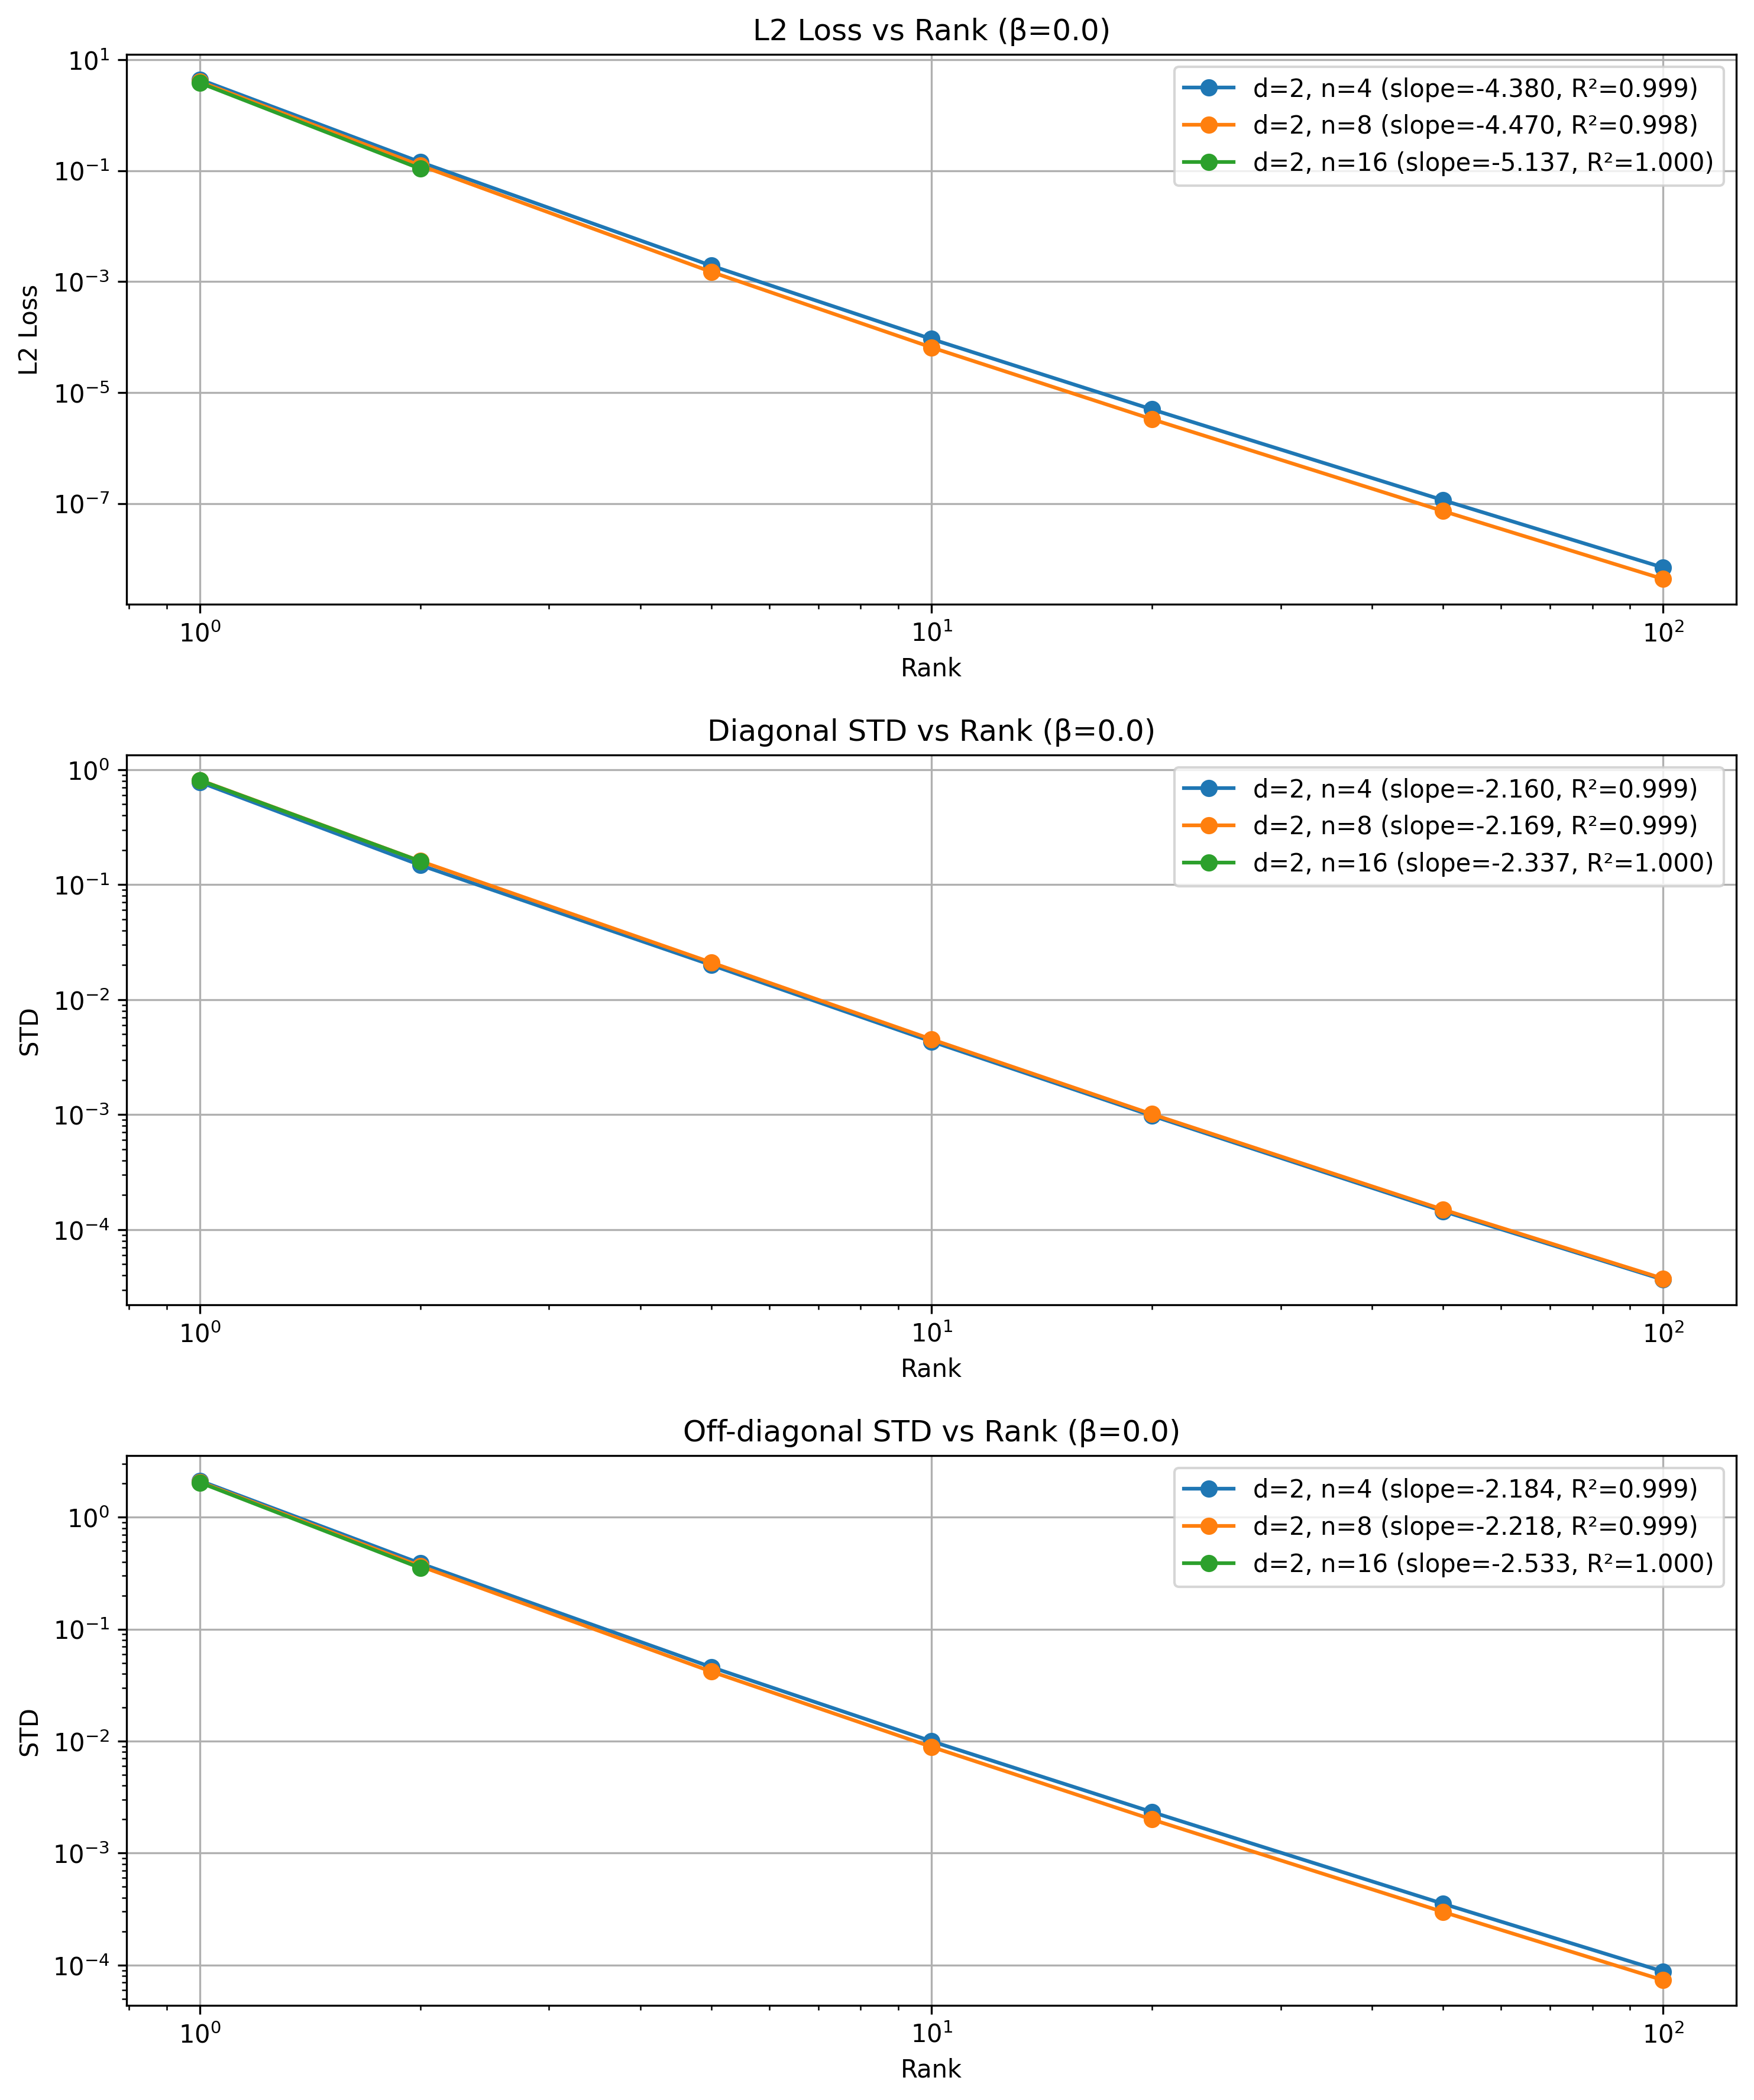
\includegraphics[width=\linewidth,height=0.50\textheight,keepaspectratio]{rank_scaling_beta0.png}
    \end{column}
    \begin{column}{0.49\textwidth}
      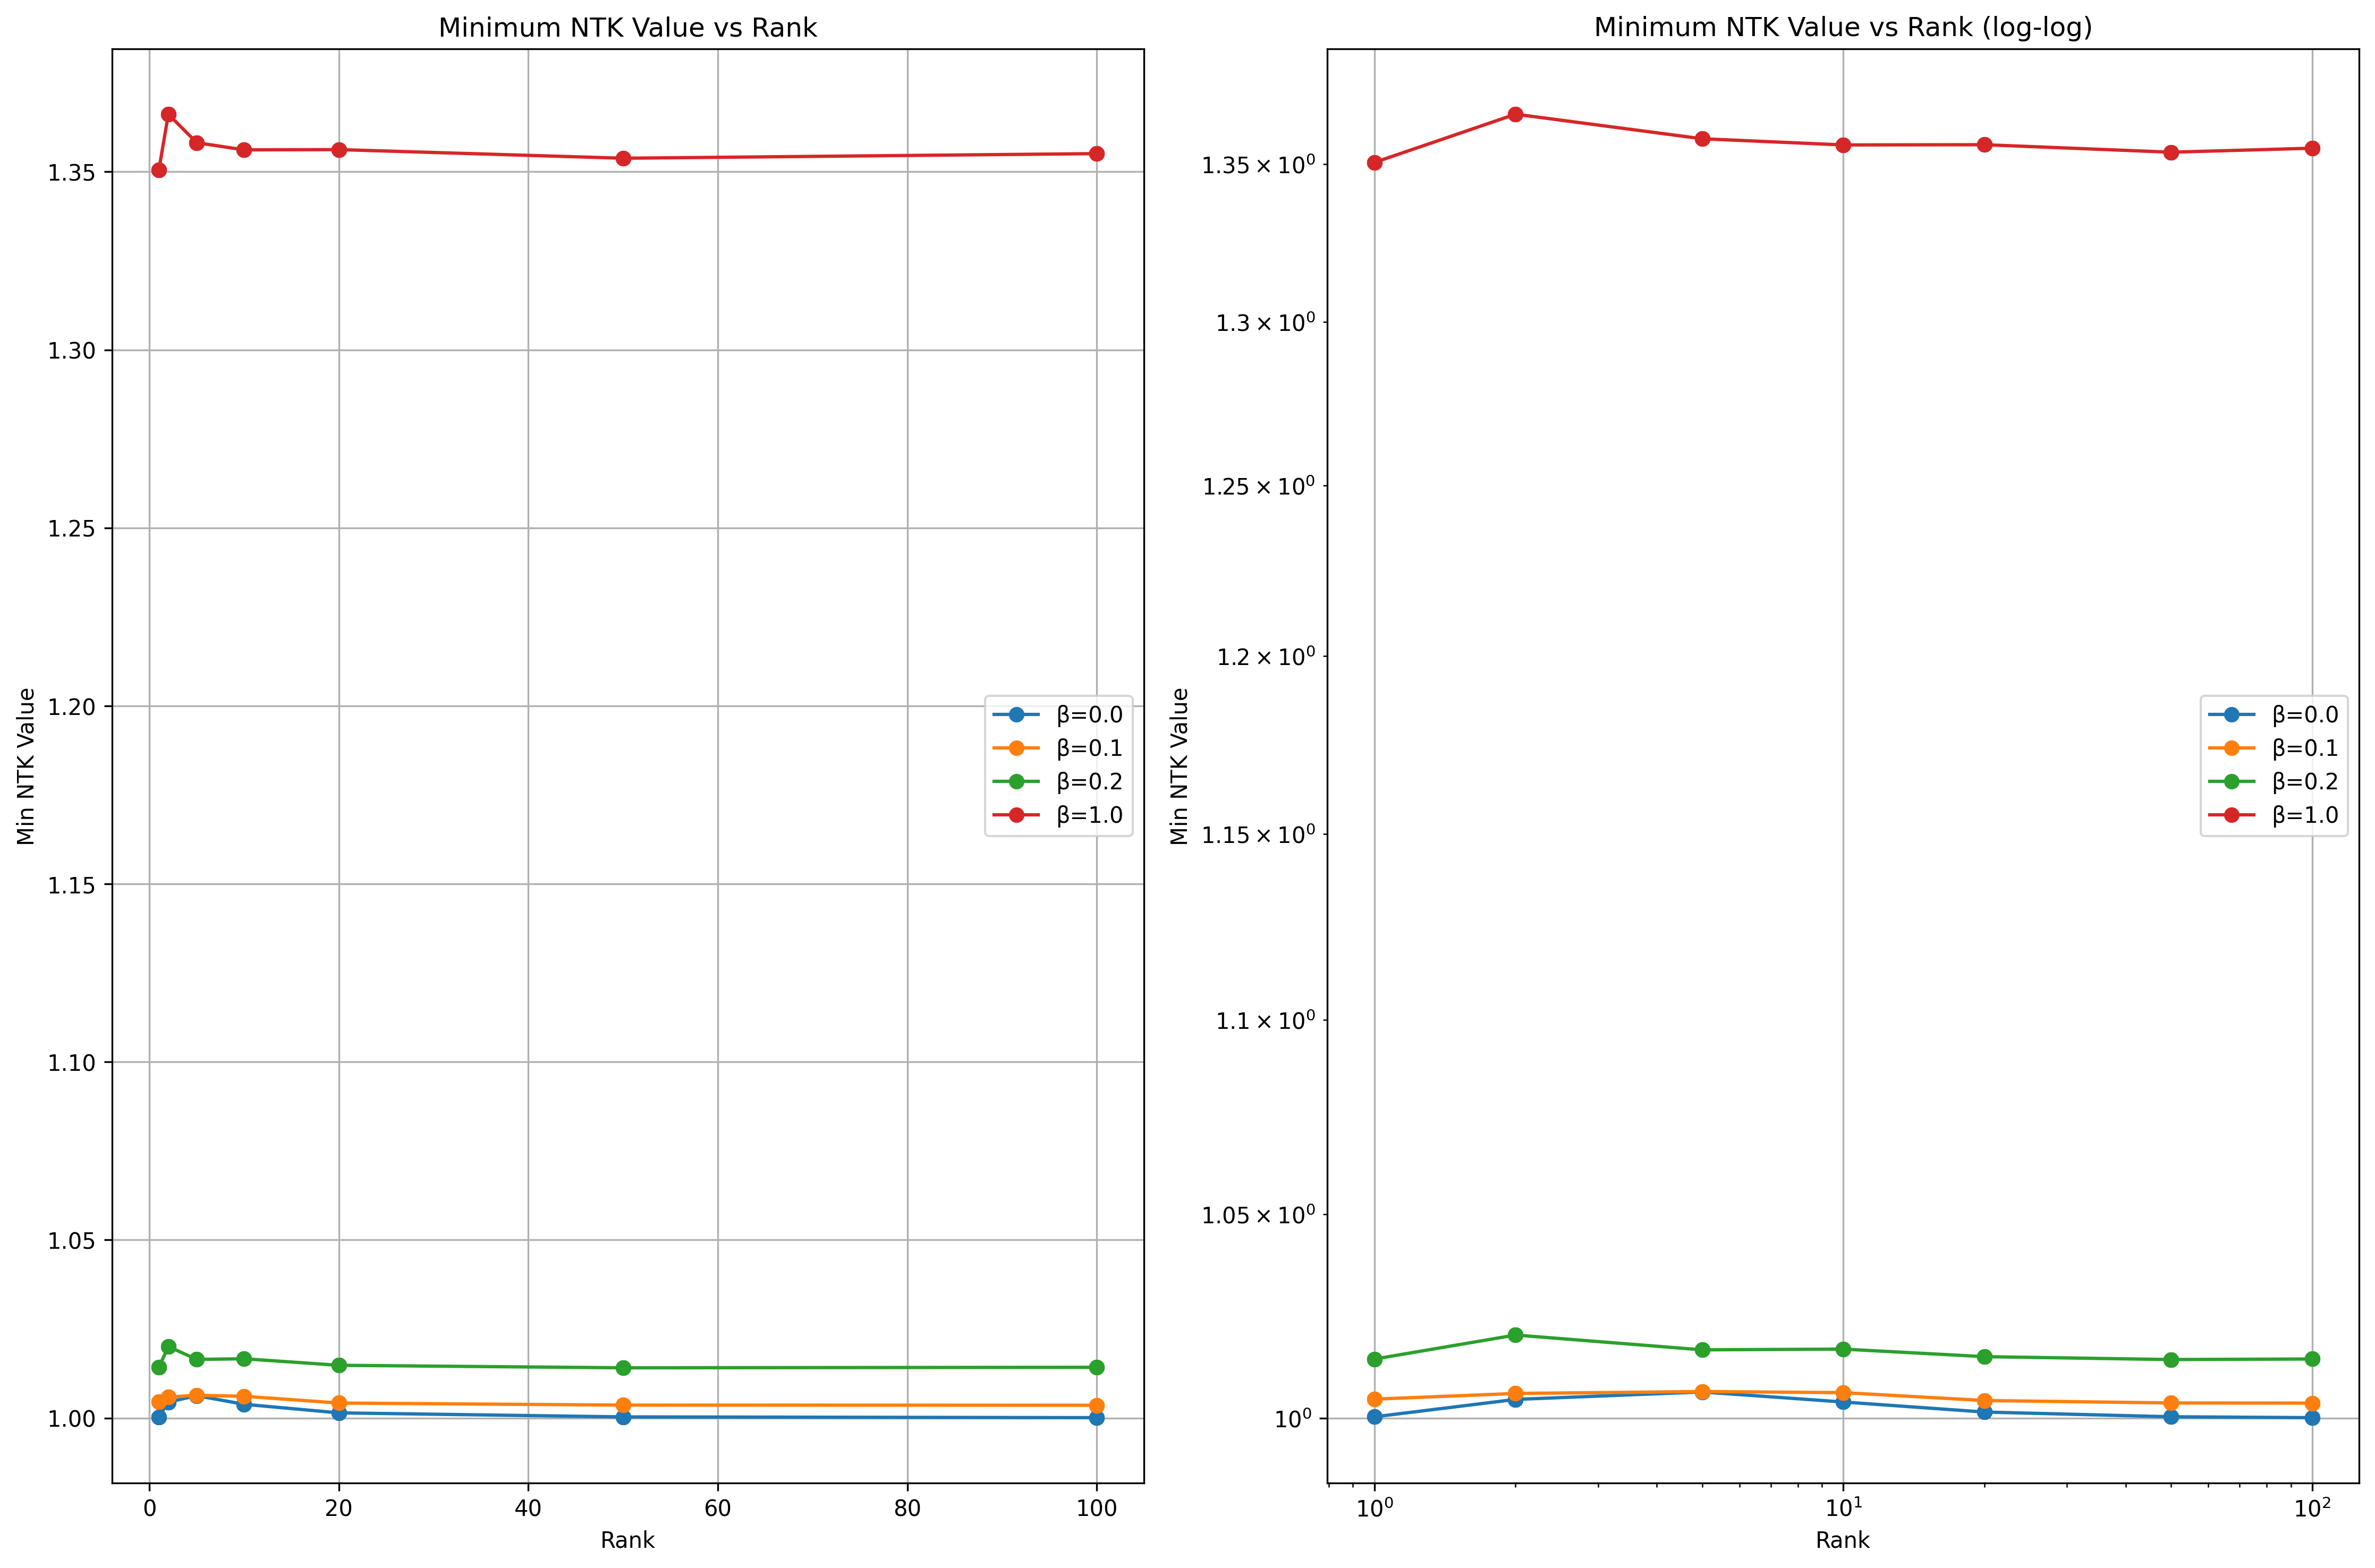
\includegraphics[width=\linewidth,height=0.50\textheight,keepaspectratio]{min_ntk_vs_rank.png}
    \end{column}
  \end{columns}
  \vspace{0.4em}
  \begin{itemize}
    \item Rank changes both kernel magnitude and spectral spread.
    \item The effect is already structured in the early experiments.
    \item These plots motivated the later theory.
    \item The subsequent results explain this empirical pattern.
  \end{itemize}
\end{frame}

\begin{frame}{Spectrum Comparison}
  \begin{columns}[T]
    \begin{column}{0.58\textwidth}
      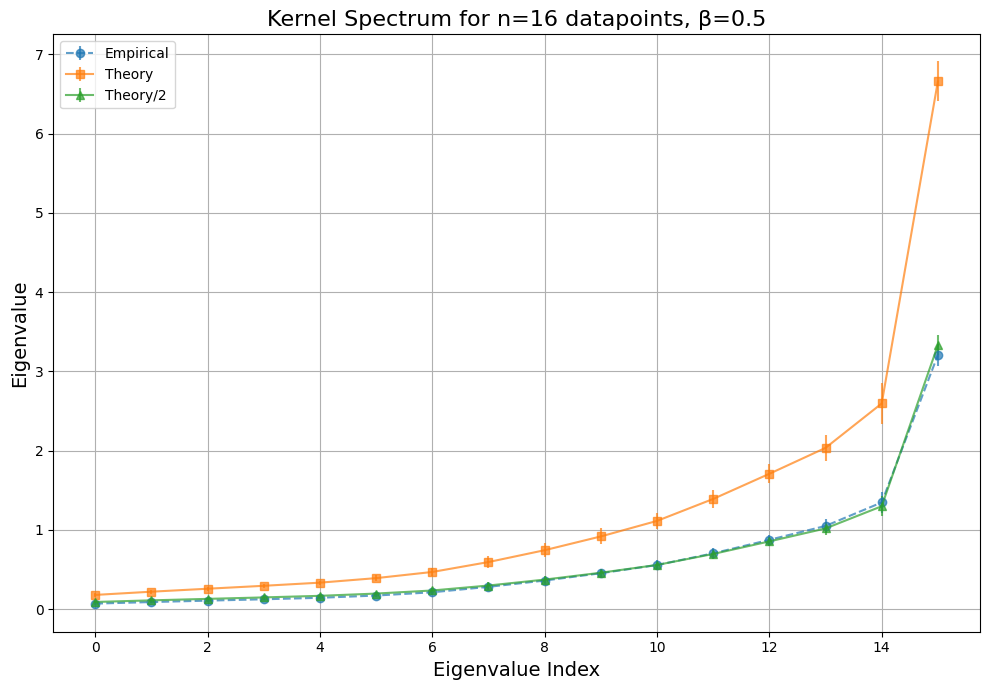
\includegraphics[width=\linewidth,height=0.52\textheight,keepaspectratio]{kernelspectrum_mlp_mmnn.png}
    \end{column}
    \begin{column}{0.38\textwidth}
      \begin{itemize}
        \item The MMNN spectrum approaches the MLP benchmark systematically.
        \item Increasing rank sharpens concentration.
        \item The comparison persists across scales.
        \item This suggests a genuine spectral correspondence.
      \end{itemize}
    \end{column}
  \end{columns}
\end{frame}

\begin{frame}{Kernel Statistics Beyond the Mean}
  \small
  \begin{columns}[T]
    \begin{column}{0.49\textwidth}
      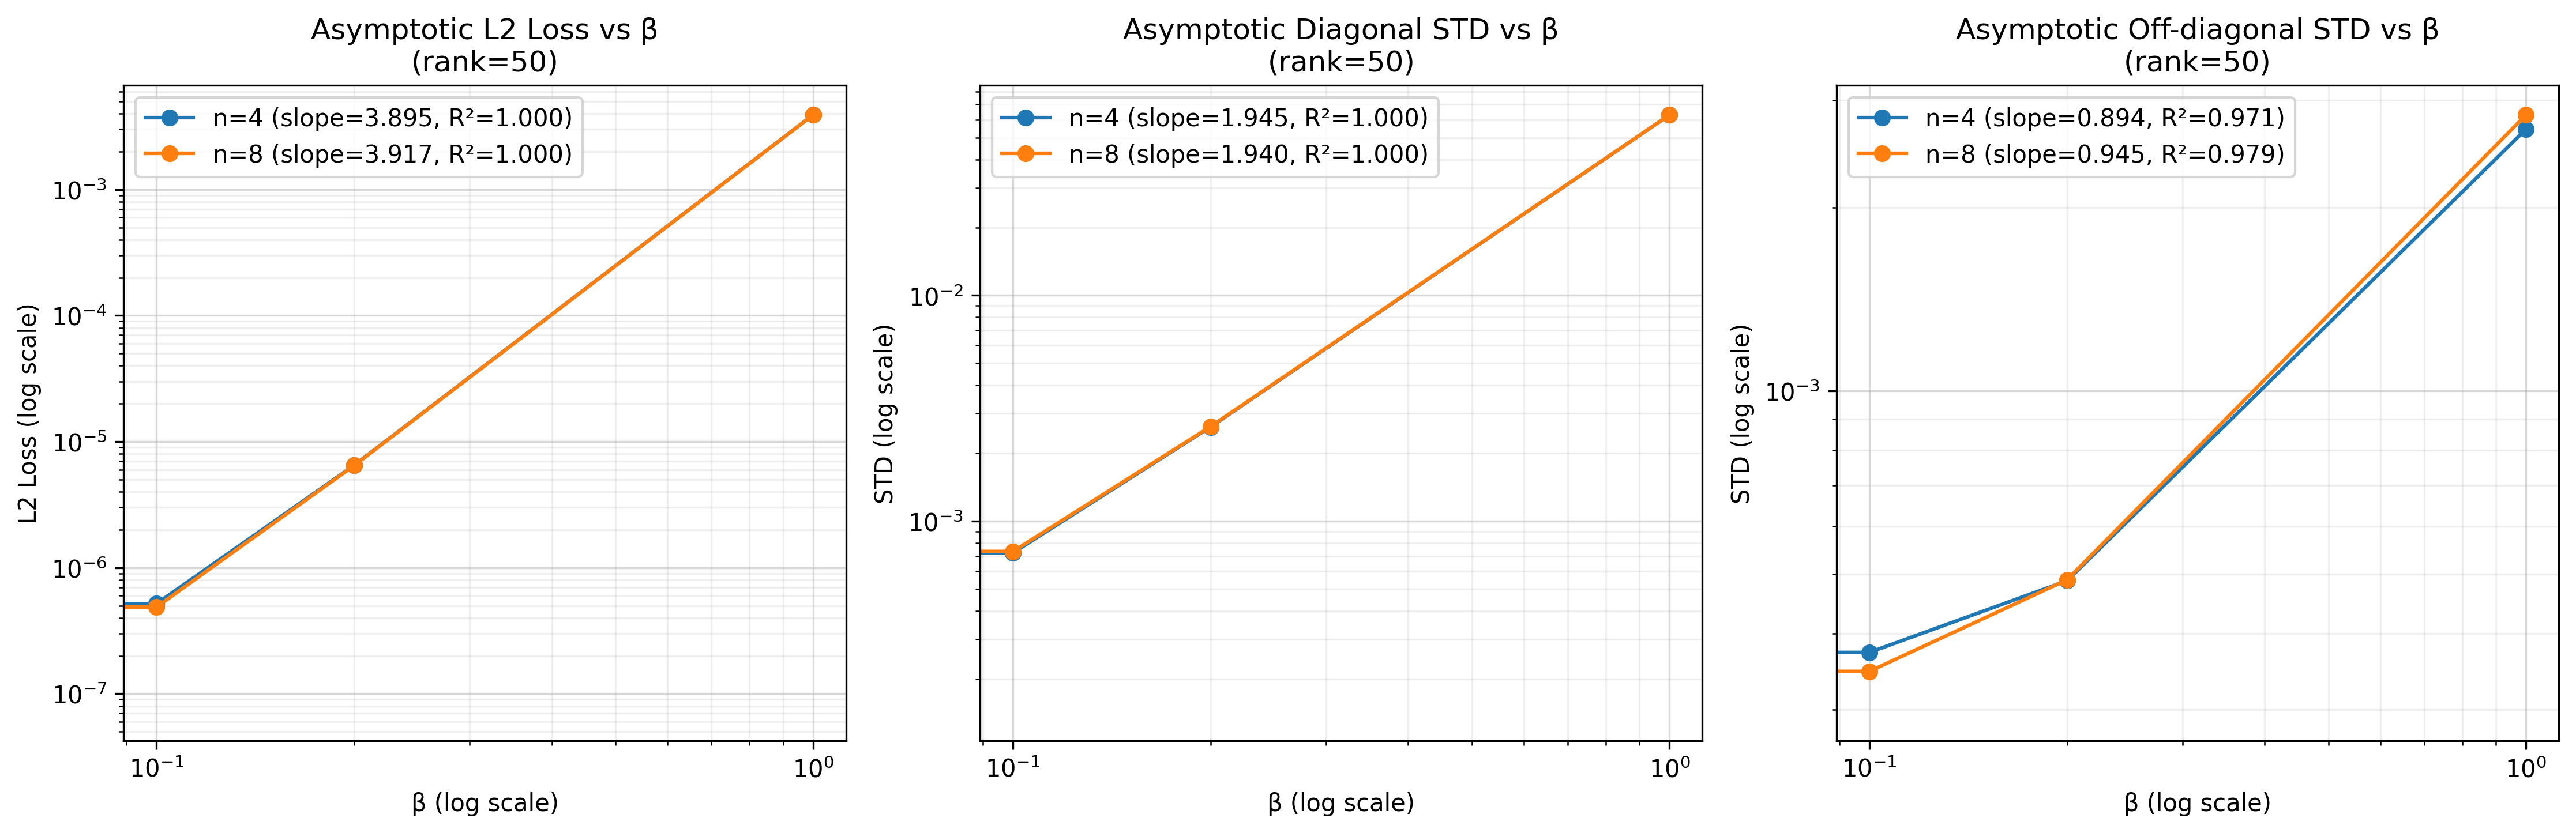
\includegraphics[width=\linewidth,height=0.29\textheight,keepaspectratio]{convergence_vs_beta_rank50.png}
    \end{column}
    \begin{column}{0.49\textwidth}
      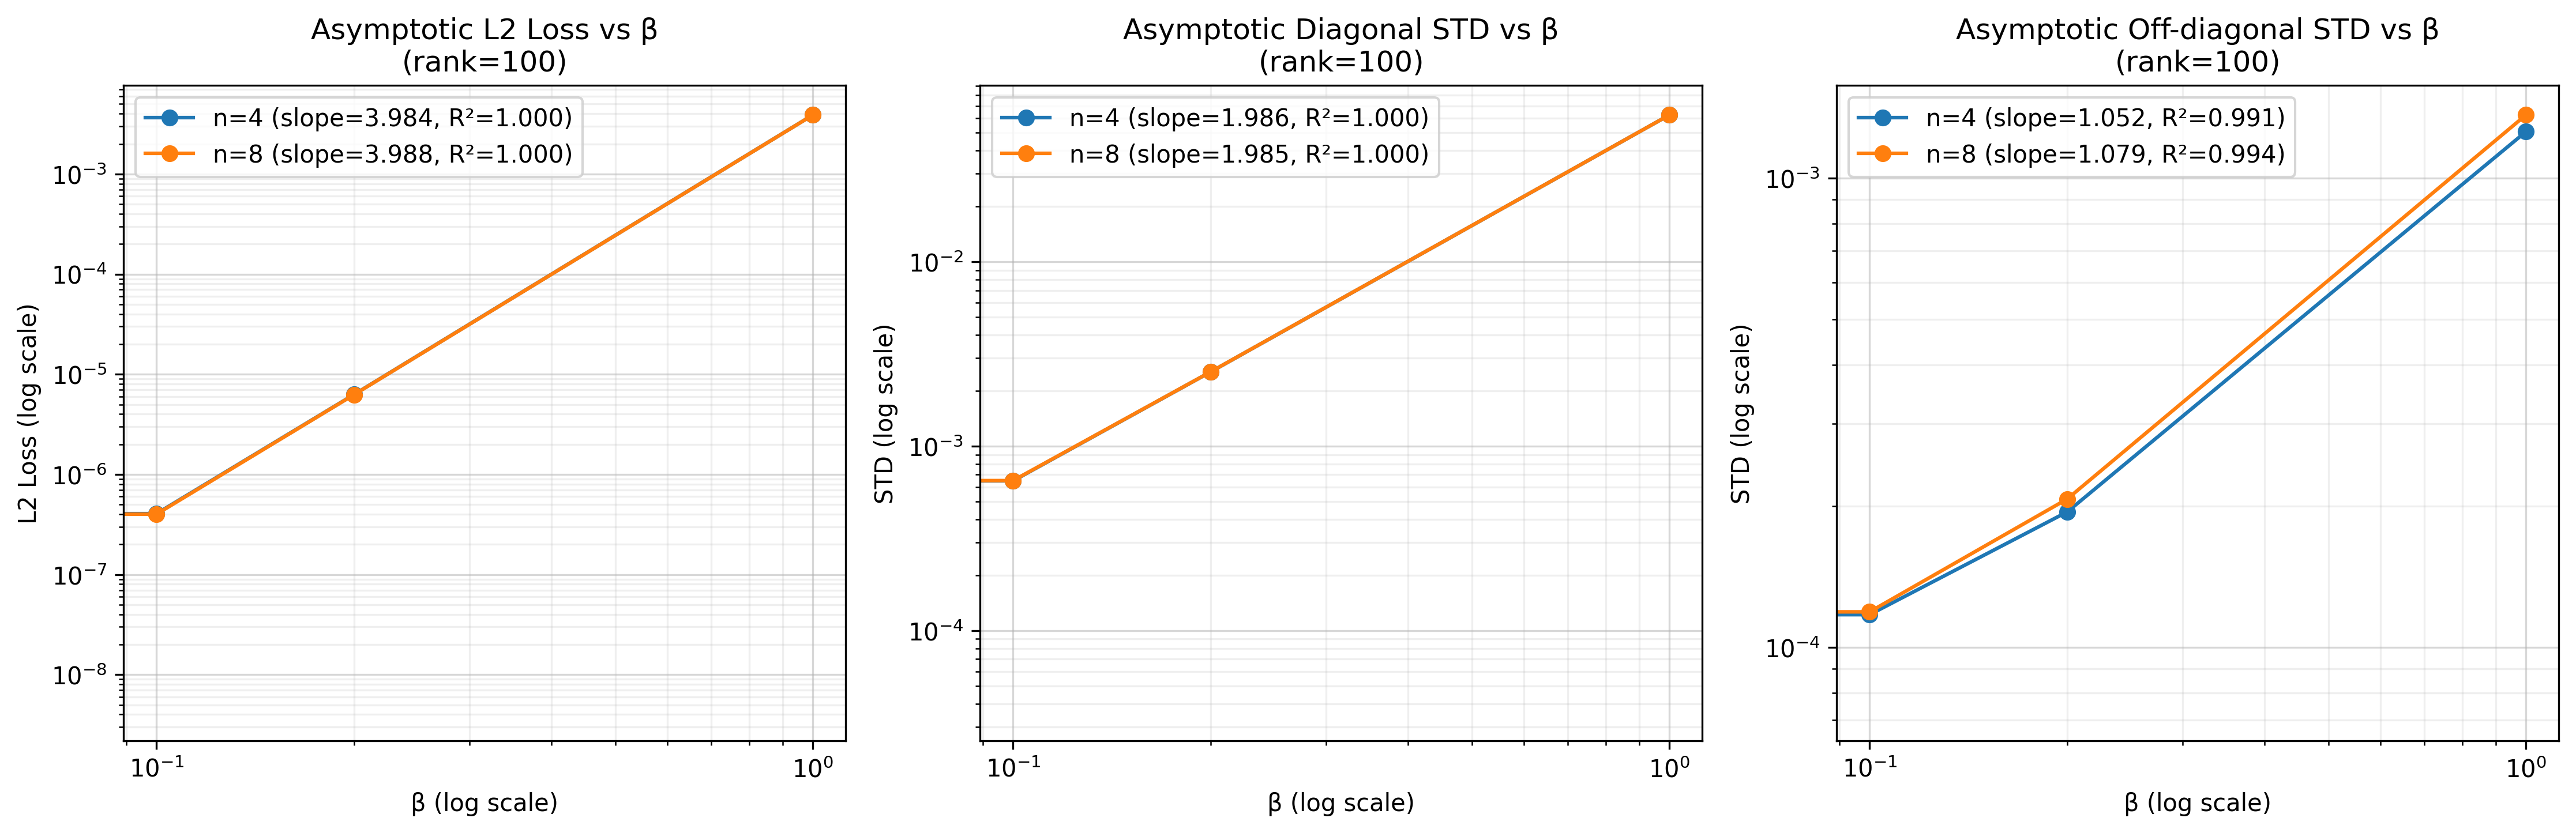
\includegraphics[width=\linewidth,height=0.29\textheight,keepaspectratio]{convergence_vs_beta_rank100.png}
    \end{column}
  \end{columns}
  \vspace{0.35em}
  \begin{columns}[T]
    \begin{column}{0.49\textwidth}
      
\includegraphics[width=\linewidth,height=0.29\textheight,keepaspectratio]{ntk_distributions_rank2_beta1.0_gaussian.png}
    \end{column}
    \begin{column}{0.49\textwidth}
      
\includegraphics[width=\linewidth,height=0.29\textheight,keepaspectratio]{ntk_distributions_rank5_beta1.0_gaussian.png}
    \end{column}
  \end{columns}
  \vspace{0.3em}
  \begin{itemize}
    \item Mean values alone are insufficient.
    \item Rank affects concentration across several statistics.
    \item The dependence on $\beta$ remains visible empirically.
    \item The distribution becomes more regular as rank grows.
  \end{itemize}
\end{frame}

\begin{frame}{Distributional View of the Kernel}
  \small
  \begin{columns}[T]
    \begin{column}{0.49\textwidth}
      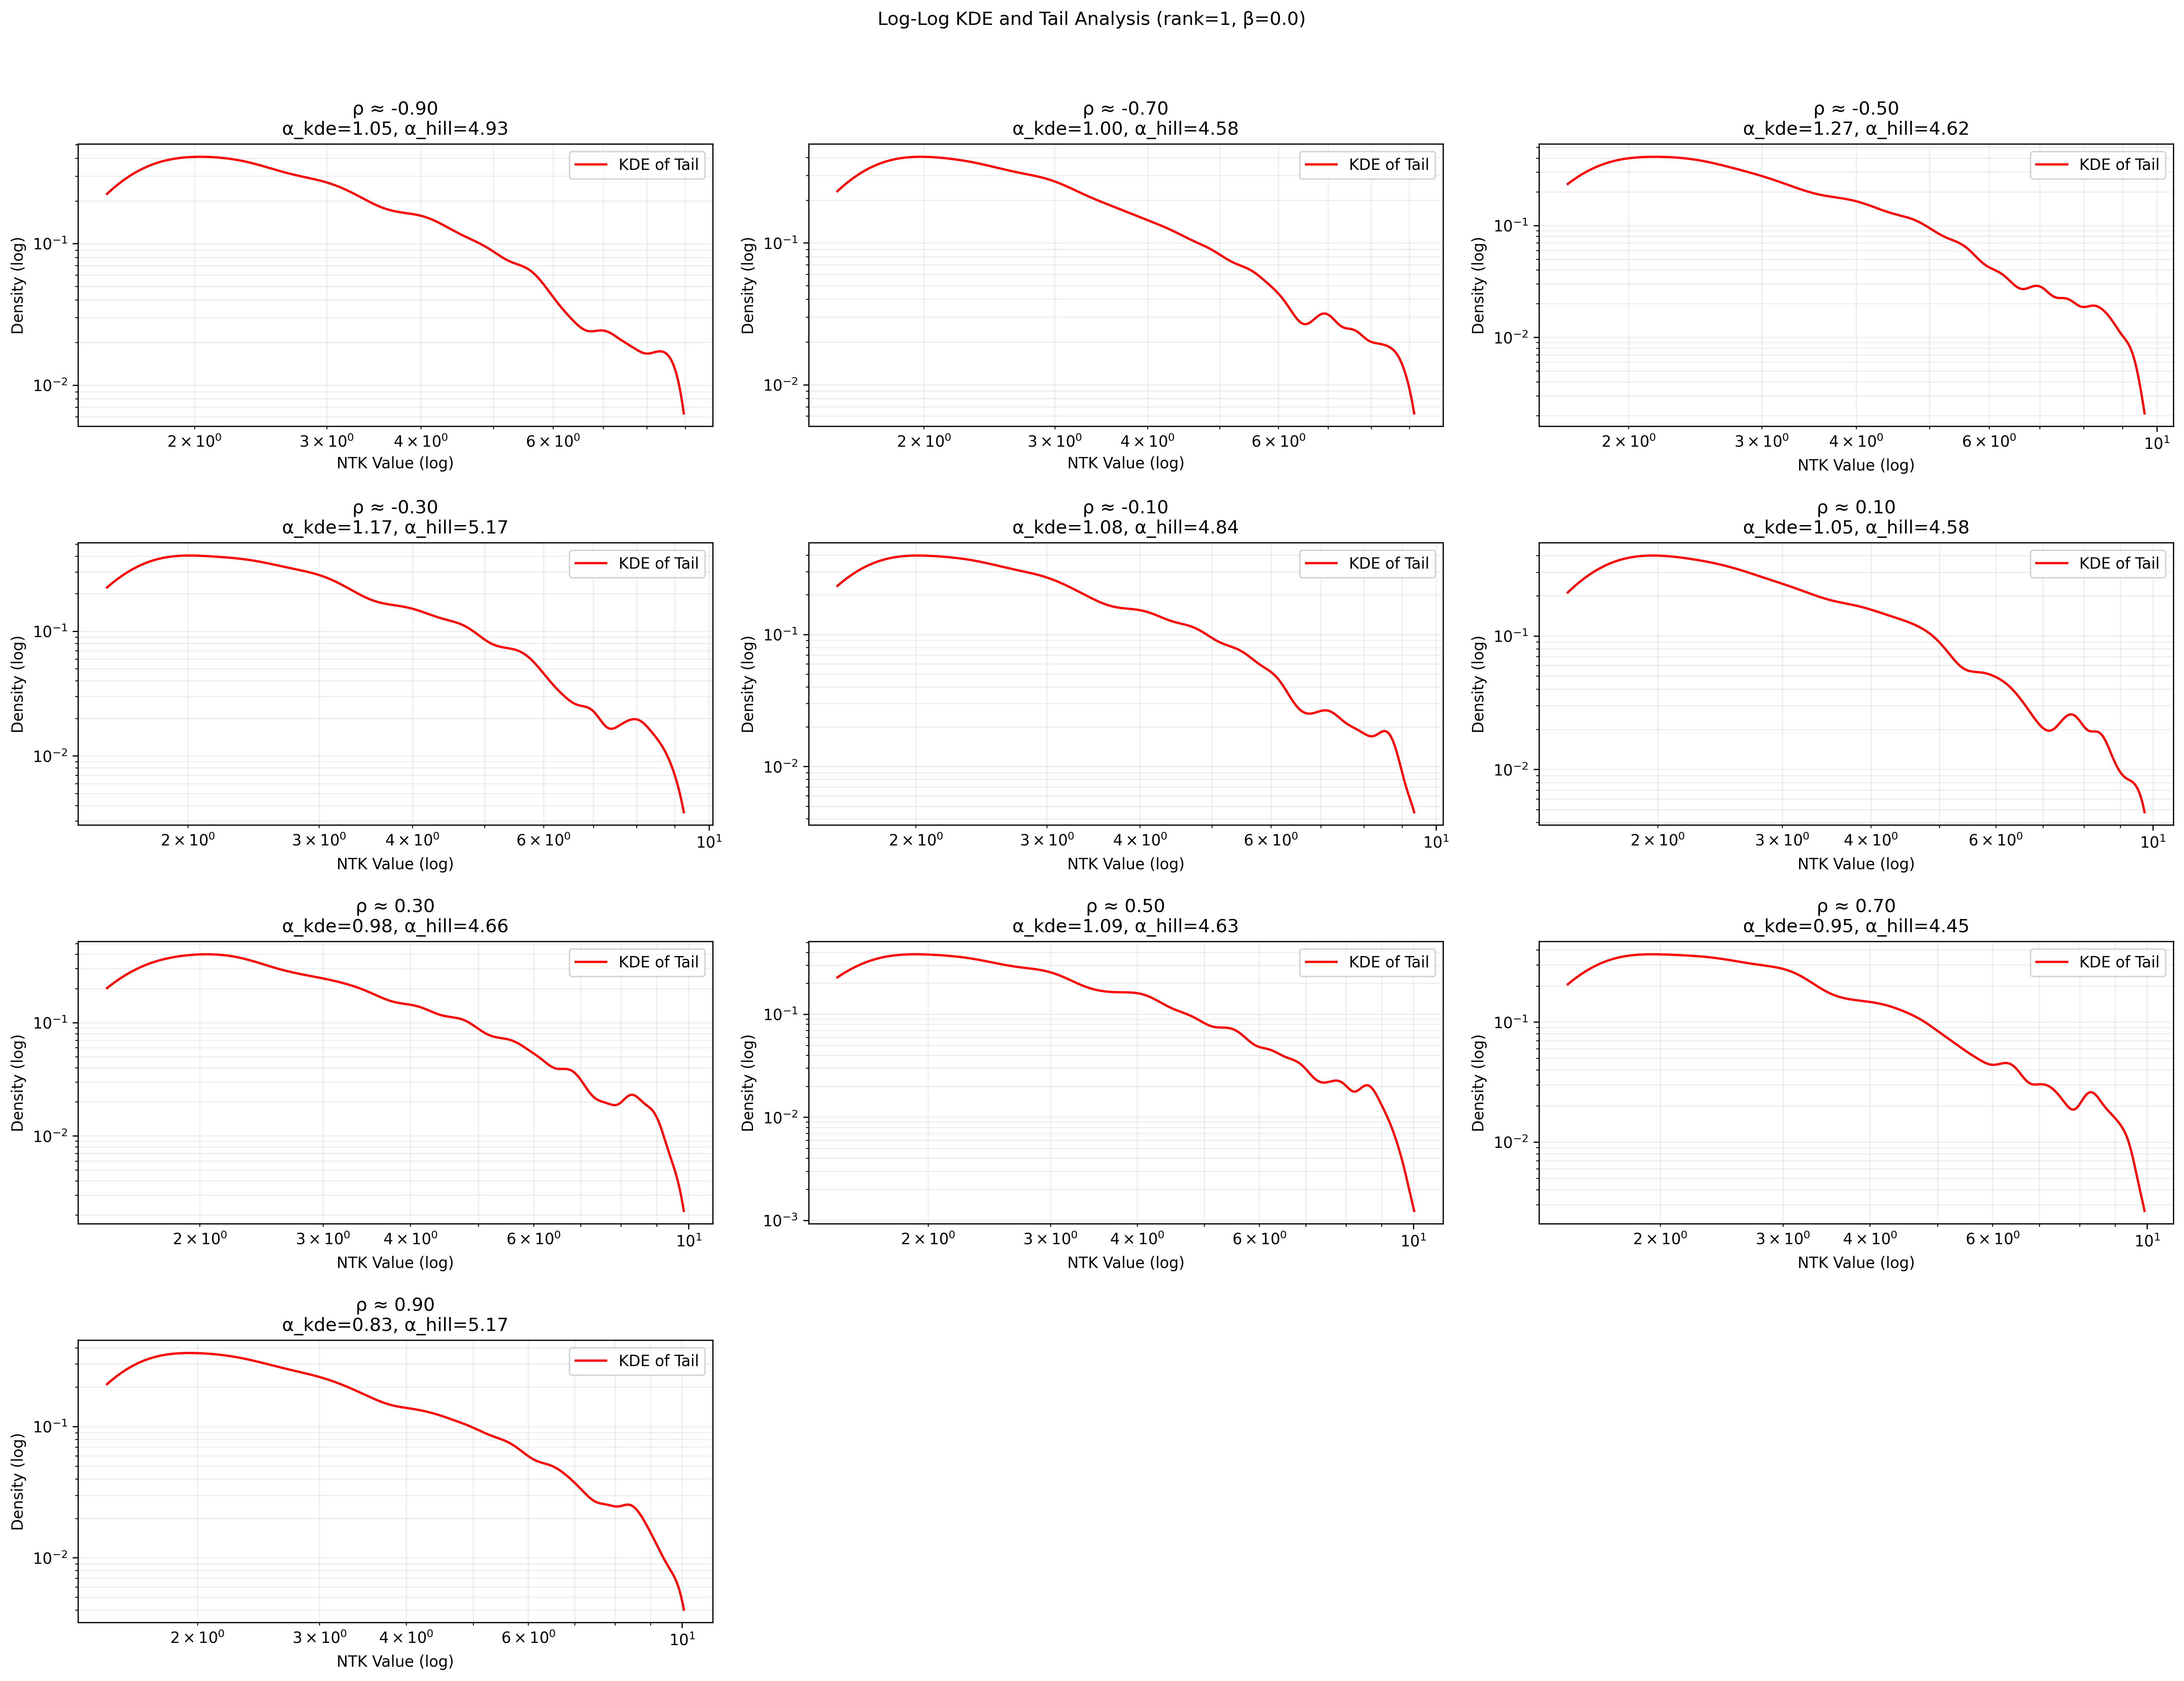
\includegraphics[width=\linewidth,height=0.50\textheight,keepaspectratio]{ntk_loglog_kde_rank1_beta0.0_gaussian.png}
    \end{column}
    \begin{column}{0.49\textwidth}
      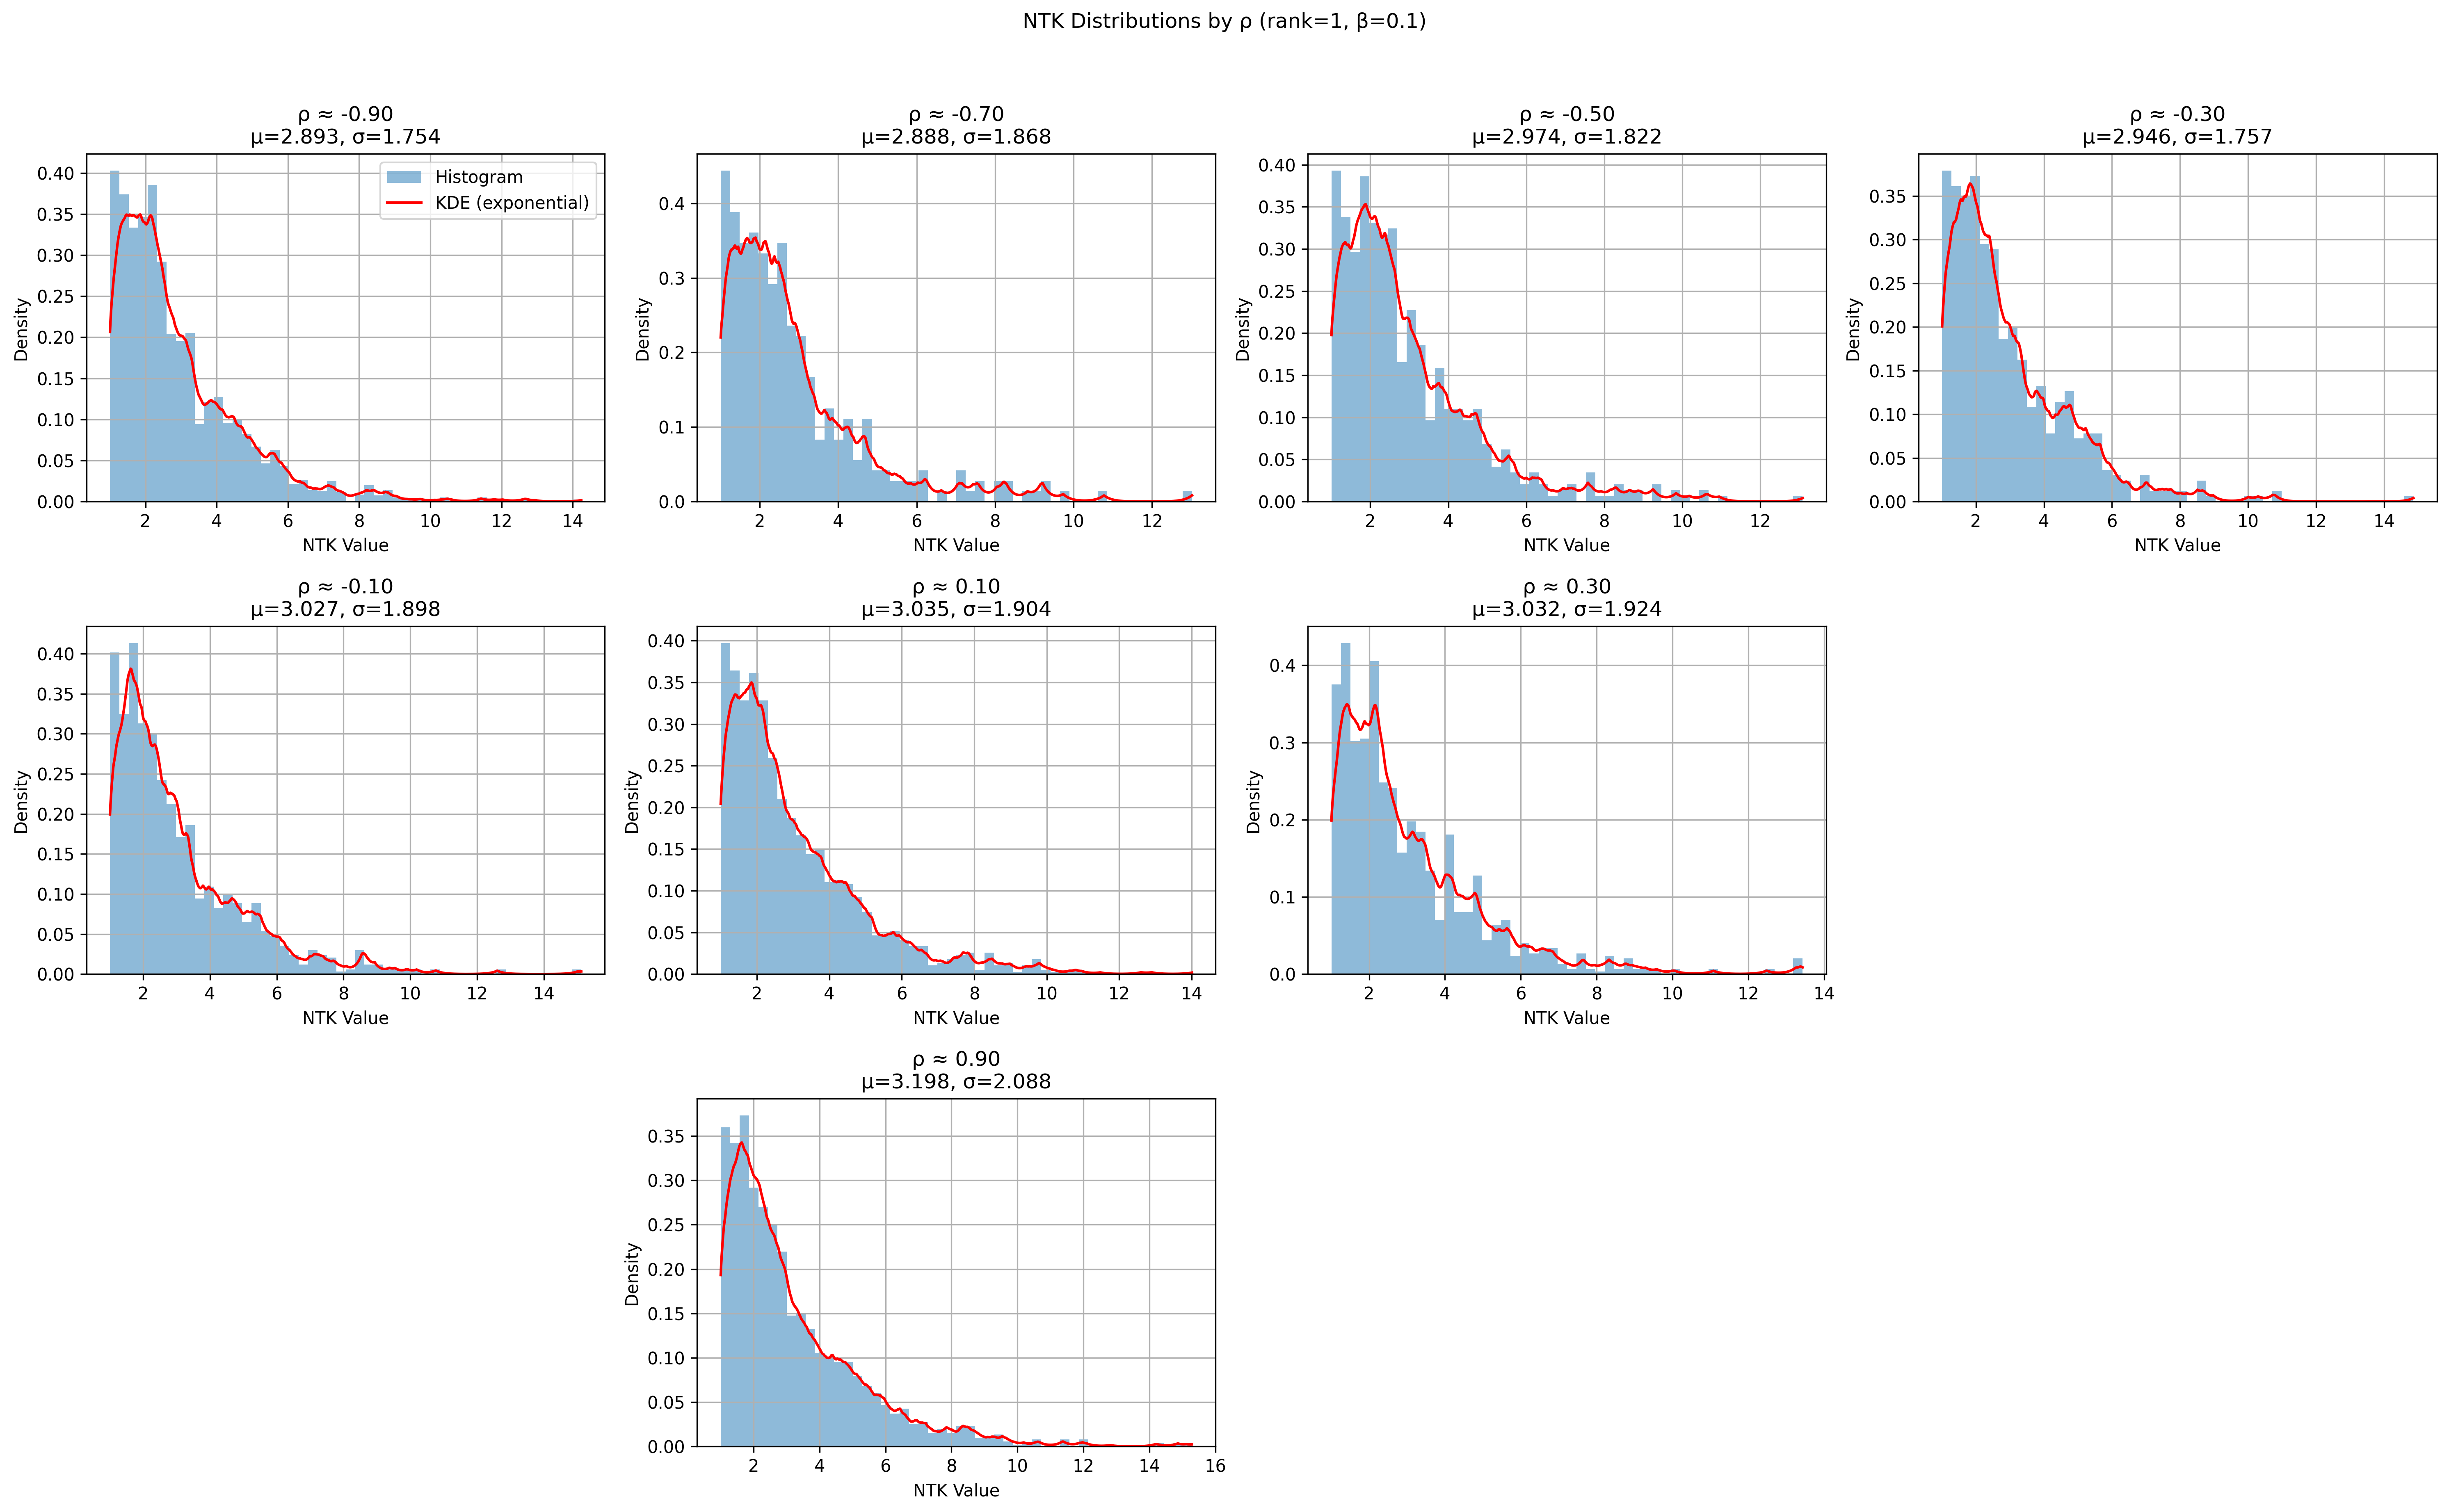
\includegraphics[width=\linewidth,height=0.50\textheight,keepaspectratio]{ntk_distributions_by_rho_rank1_beta0.1_exponential_bw0.2.png}
    \end{column}
  \end{columns}
  \vspace{0.4em}
  \begin{itemize}
    \item Mean behavior hides relevant instability.
    \item The full distribution reveals heavy tails and sensitivity.
    \item Geometry changes the location of the mass.
    \item This helps explain unstable initializations.
  \end{itemize}
\end{frame}

\begin{frame}{Feature Learning and Landscape Dynamics}
  \begin{columns}[T]
    \begin{column}{0.49\textwidth}
      
\includegraphics[width=\linewidth]{four_setups_loss_with_lr_bars.png}
    \end{column}
    \begin{column}{0.49\textwidth}
      
\includegraphics[width=\linewidth]{trajectory_max_ratio.png}
    \end{column}
  \end{columns}
  \vspace{0.4em}
  \begin{itemize}
    \item Training is not only smooth kernel descent.
    \item Plateaus and sharp drops are clearly visible.
    \item Channel specialization appears during optimization.
    \item Log-ratios connect these effects to theory.
  \end{itemize}
\end{frame}

\begin{frame}{Representation Learning Through Training}
  \small
  \begin{columns}[T]
    \begin{column}{0.49\textwidth}
      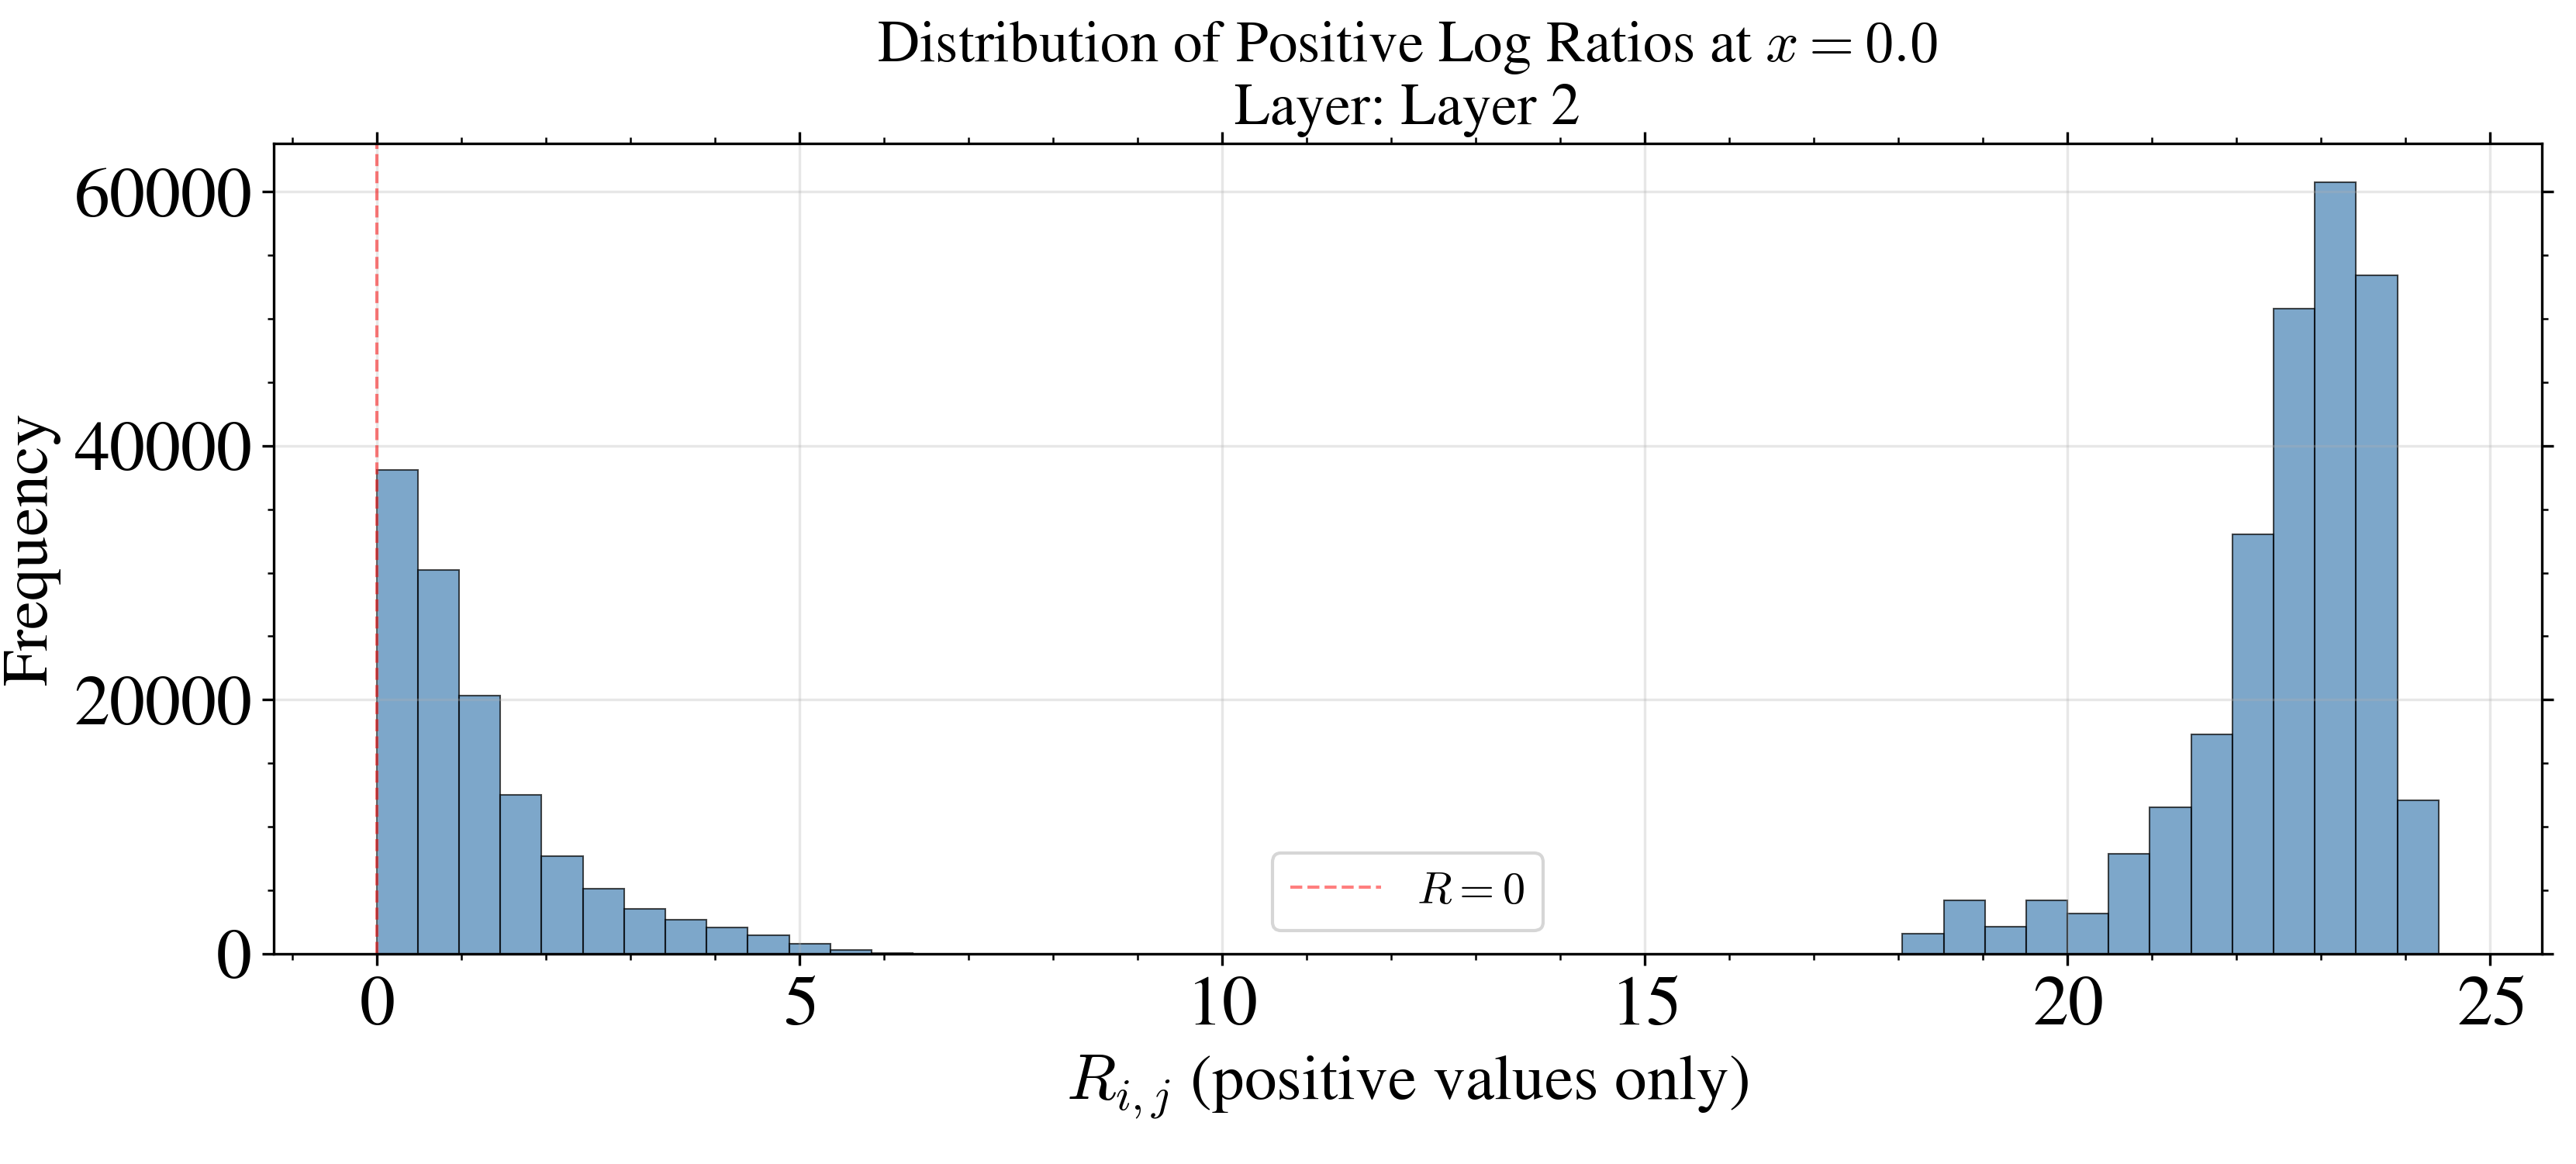
\includegraphics[width=\linewidth,height=0.30\textheight,keepaspectratio]{logratio_statistics_x0.png}
    \end{column}
    \begin{column}{0.49\textwidth}
      
\includegraphics[width=\linewidth,height=0.30\textheight,keepaspectratio]{final_prediction.png}
    \end{column}
  \end{columns}
  \vspace{0.35em}
  \begin{columns}[T]
    \begin{column}{0.49\textwidth}
      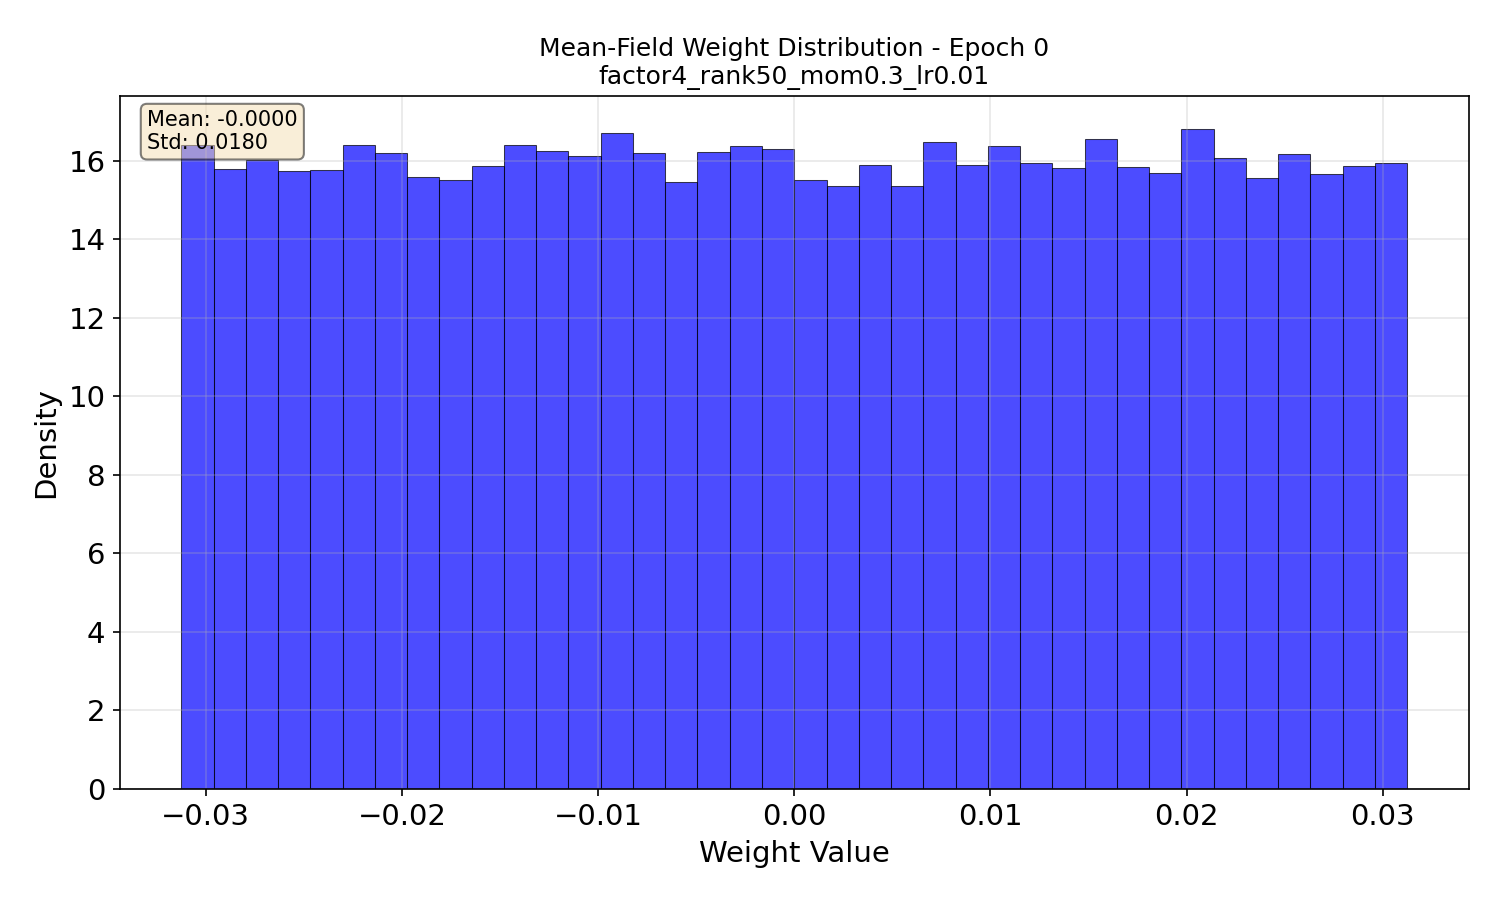
\includegraphics[width=\linewidth,height=0.25\textheight,keepaspectratio]{meanfield_density_epoch0.png}
    \end{column}
    \begin{column}{0.49\textwidth}
      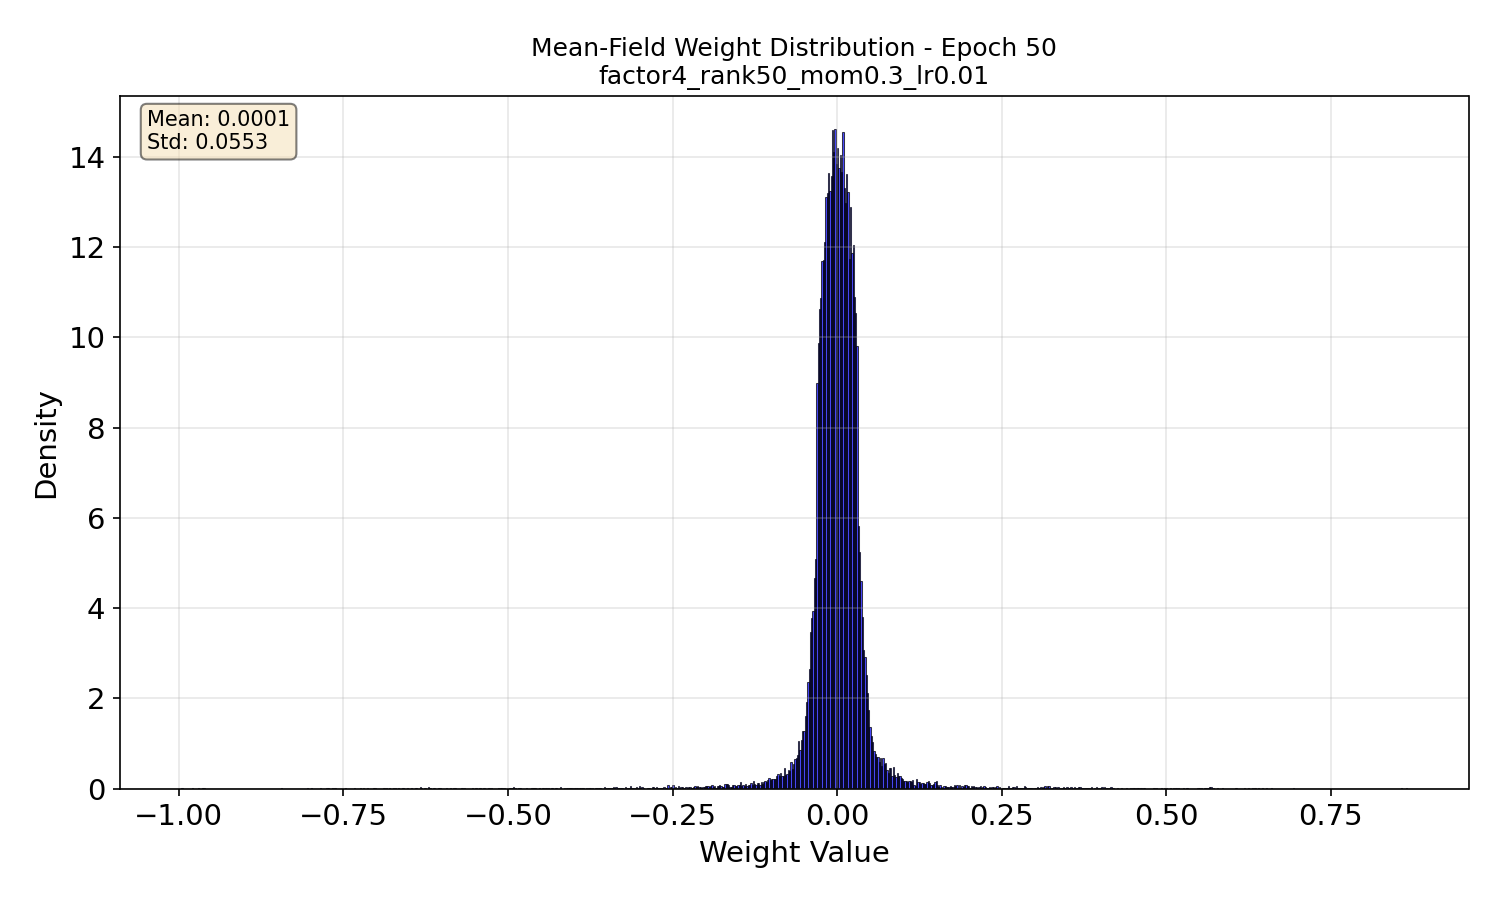
\includegraphics[width=\linewidth,height=0.25\textheight,keepaspectratio]{meanfield_density_epoch50.png}
    \end{column}
  \end{columns}
  \vspace{0.3em}
  \begin{itemize}
    \item Observables, learned functions, and mean-field motion agree.
    \item The representation moves substantially during training.
    \item This motion improves the final predictor.
    \item The regime is not purely lazy.
  \end{itemize}
\end{frame}

\begin{frame}{Internal Features Are Structured, Not Arbitrary}
  \begin{columns}[T]
    \begin{column}{0.32\textwidth}
      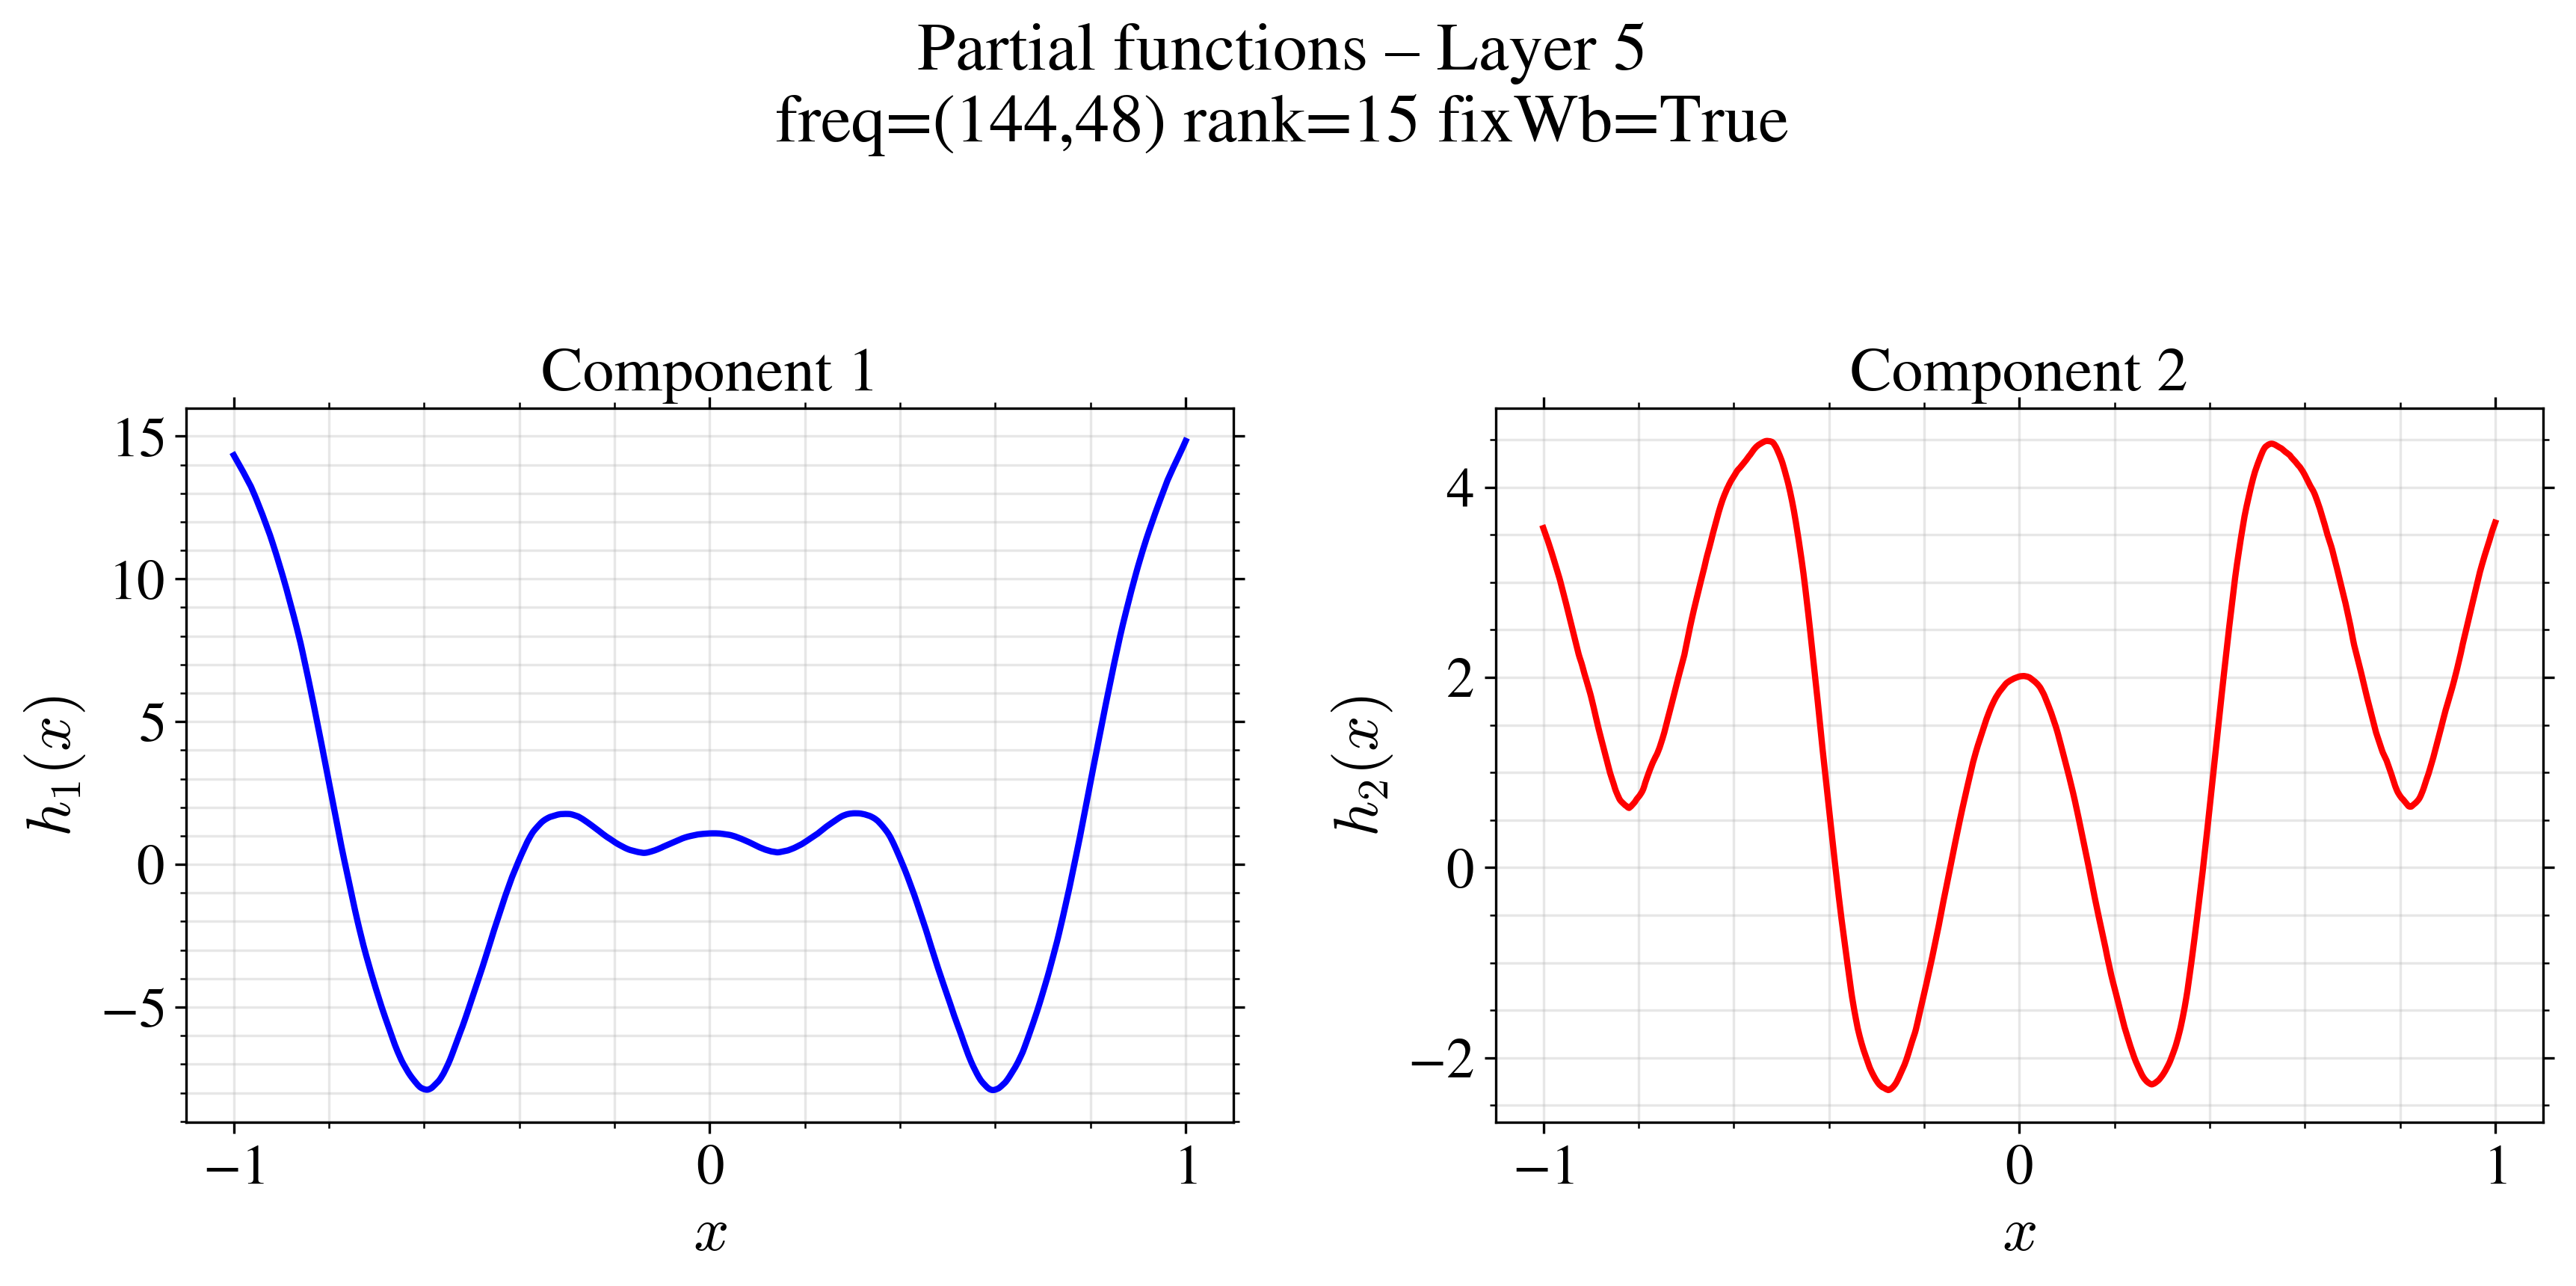
\includegraphics[width=\linewidth]{channel_partials_layer5.png}
    \end{column}
    \begin{column}{0.32\textwidth}
      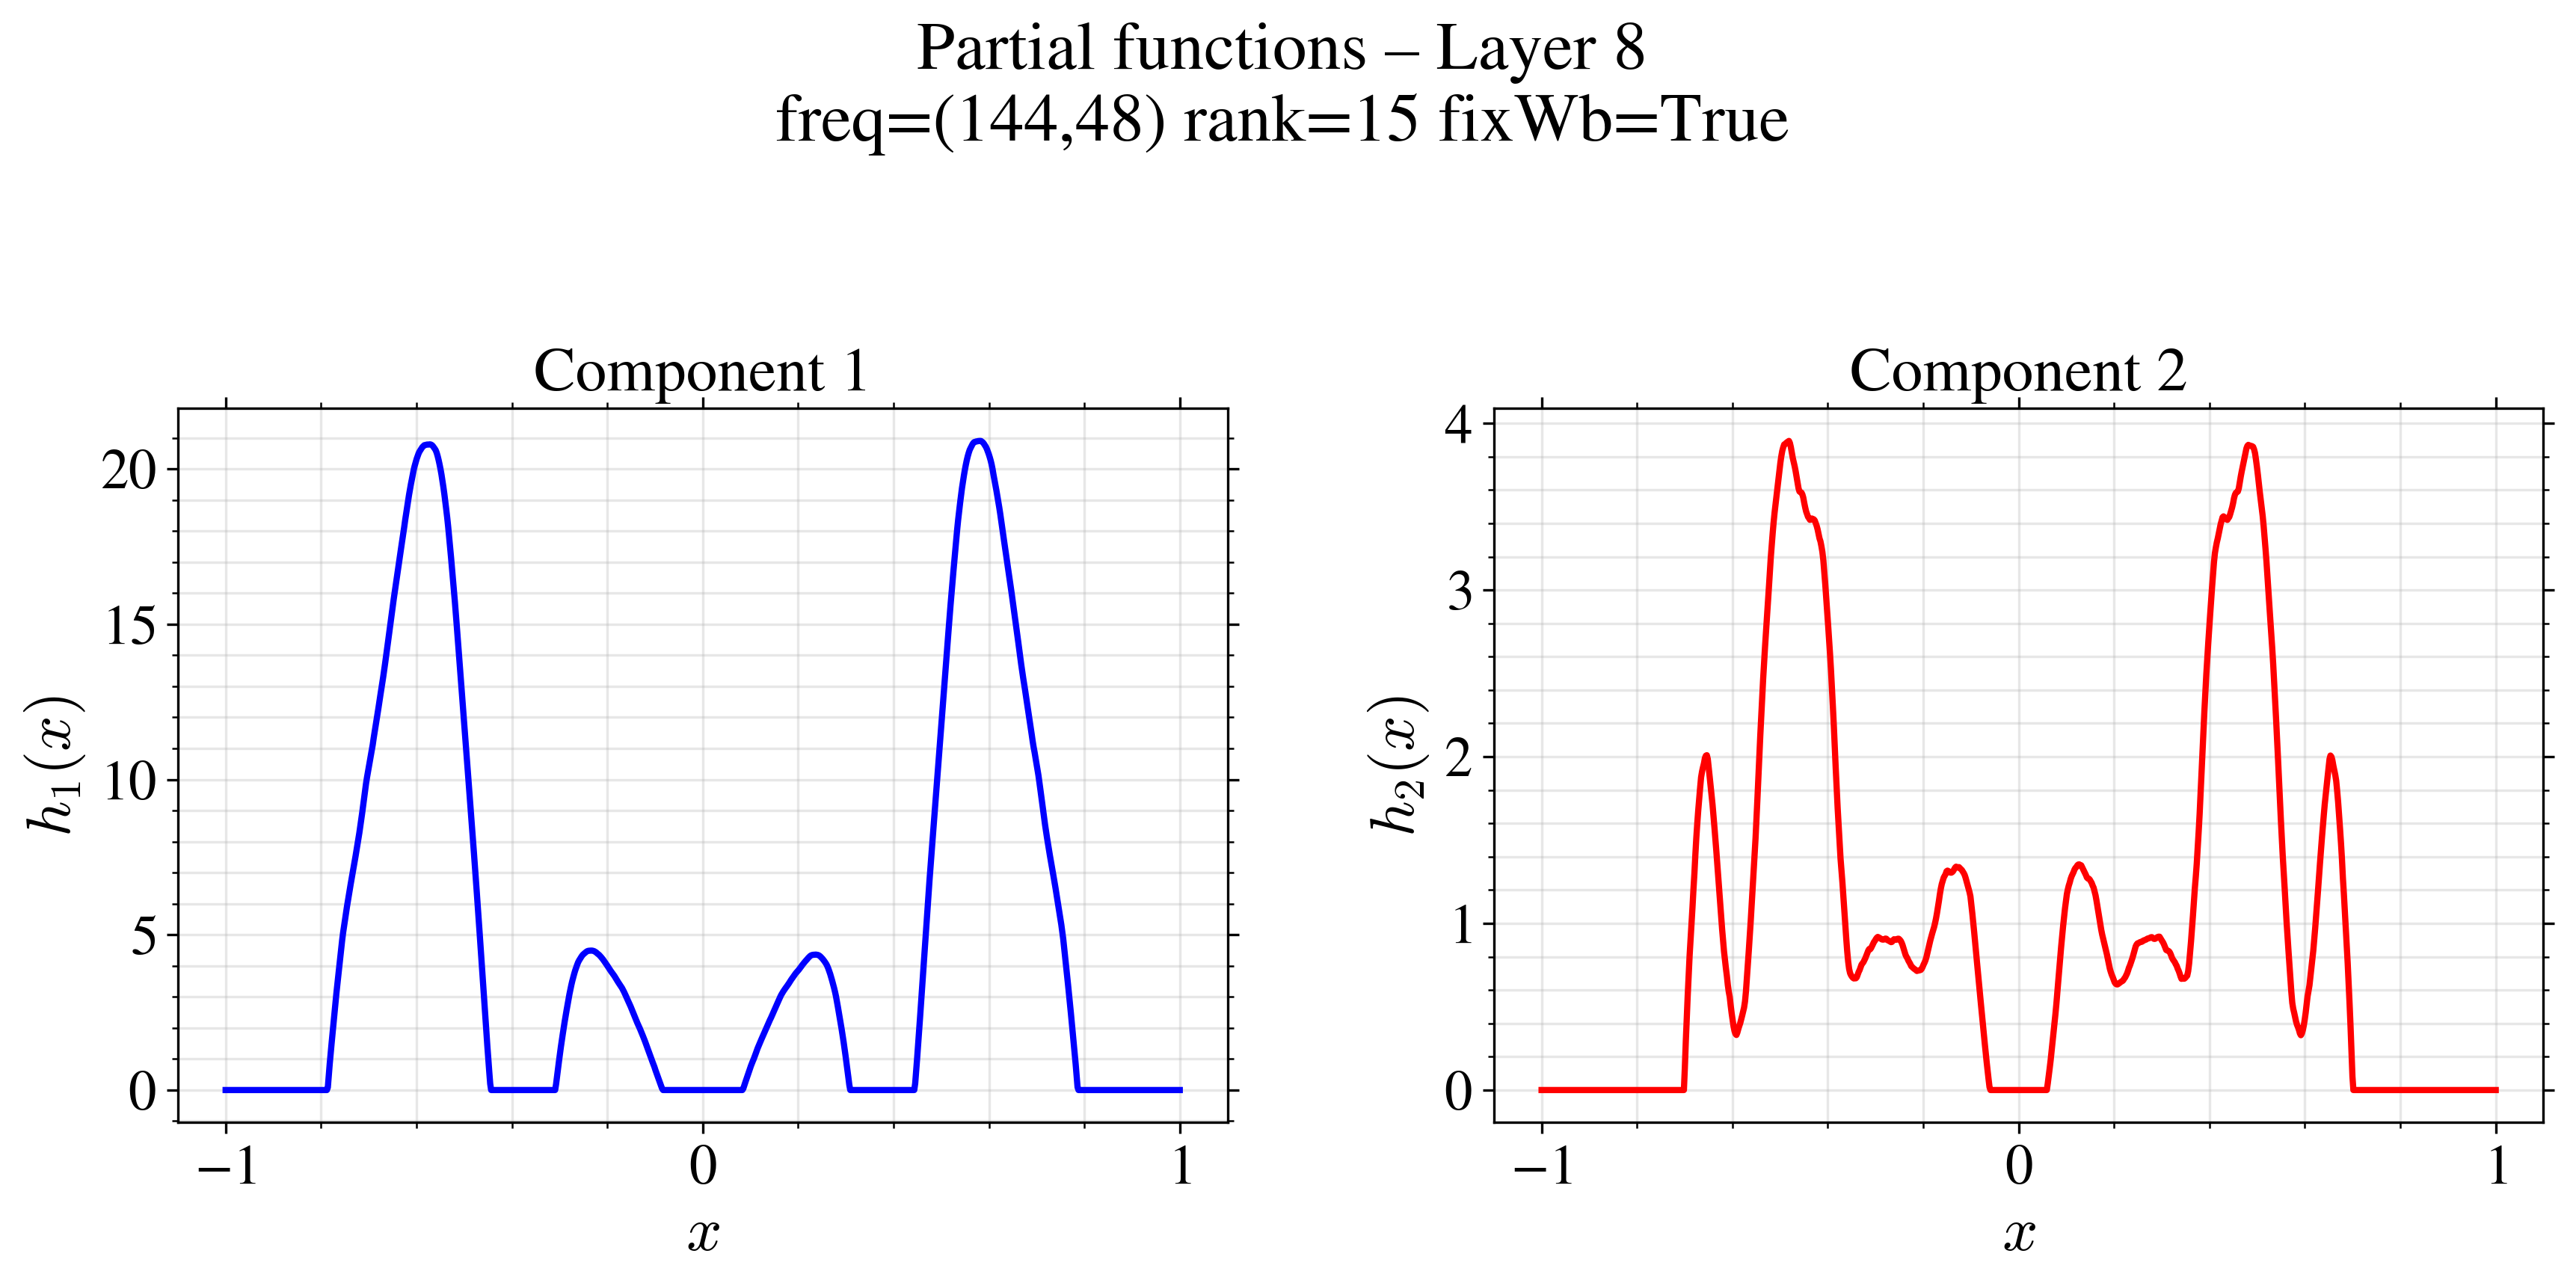
\includegraphics[width=\linewidth]{spike_in_H_layer9.png}
    \end{column}
    \begin{column}{0.32\textwidth}
      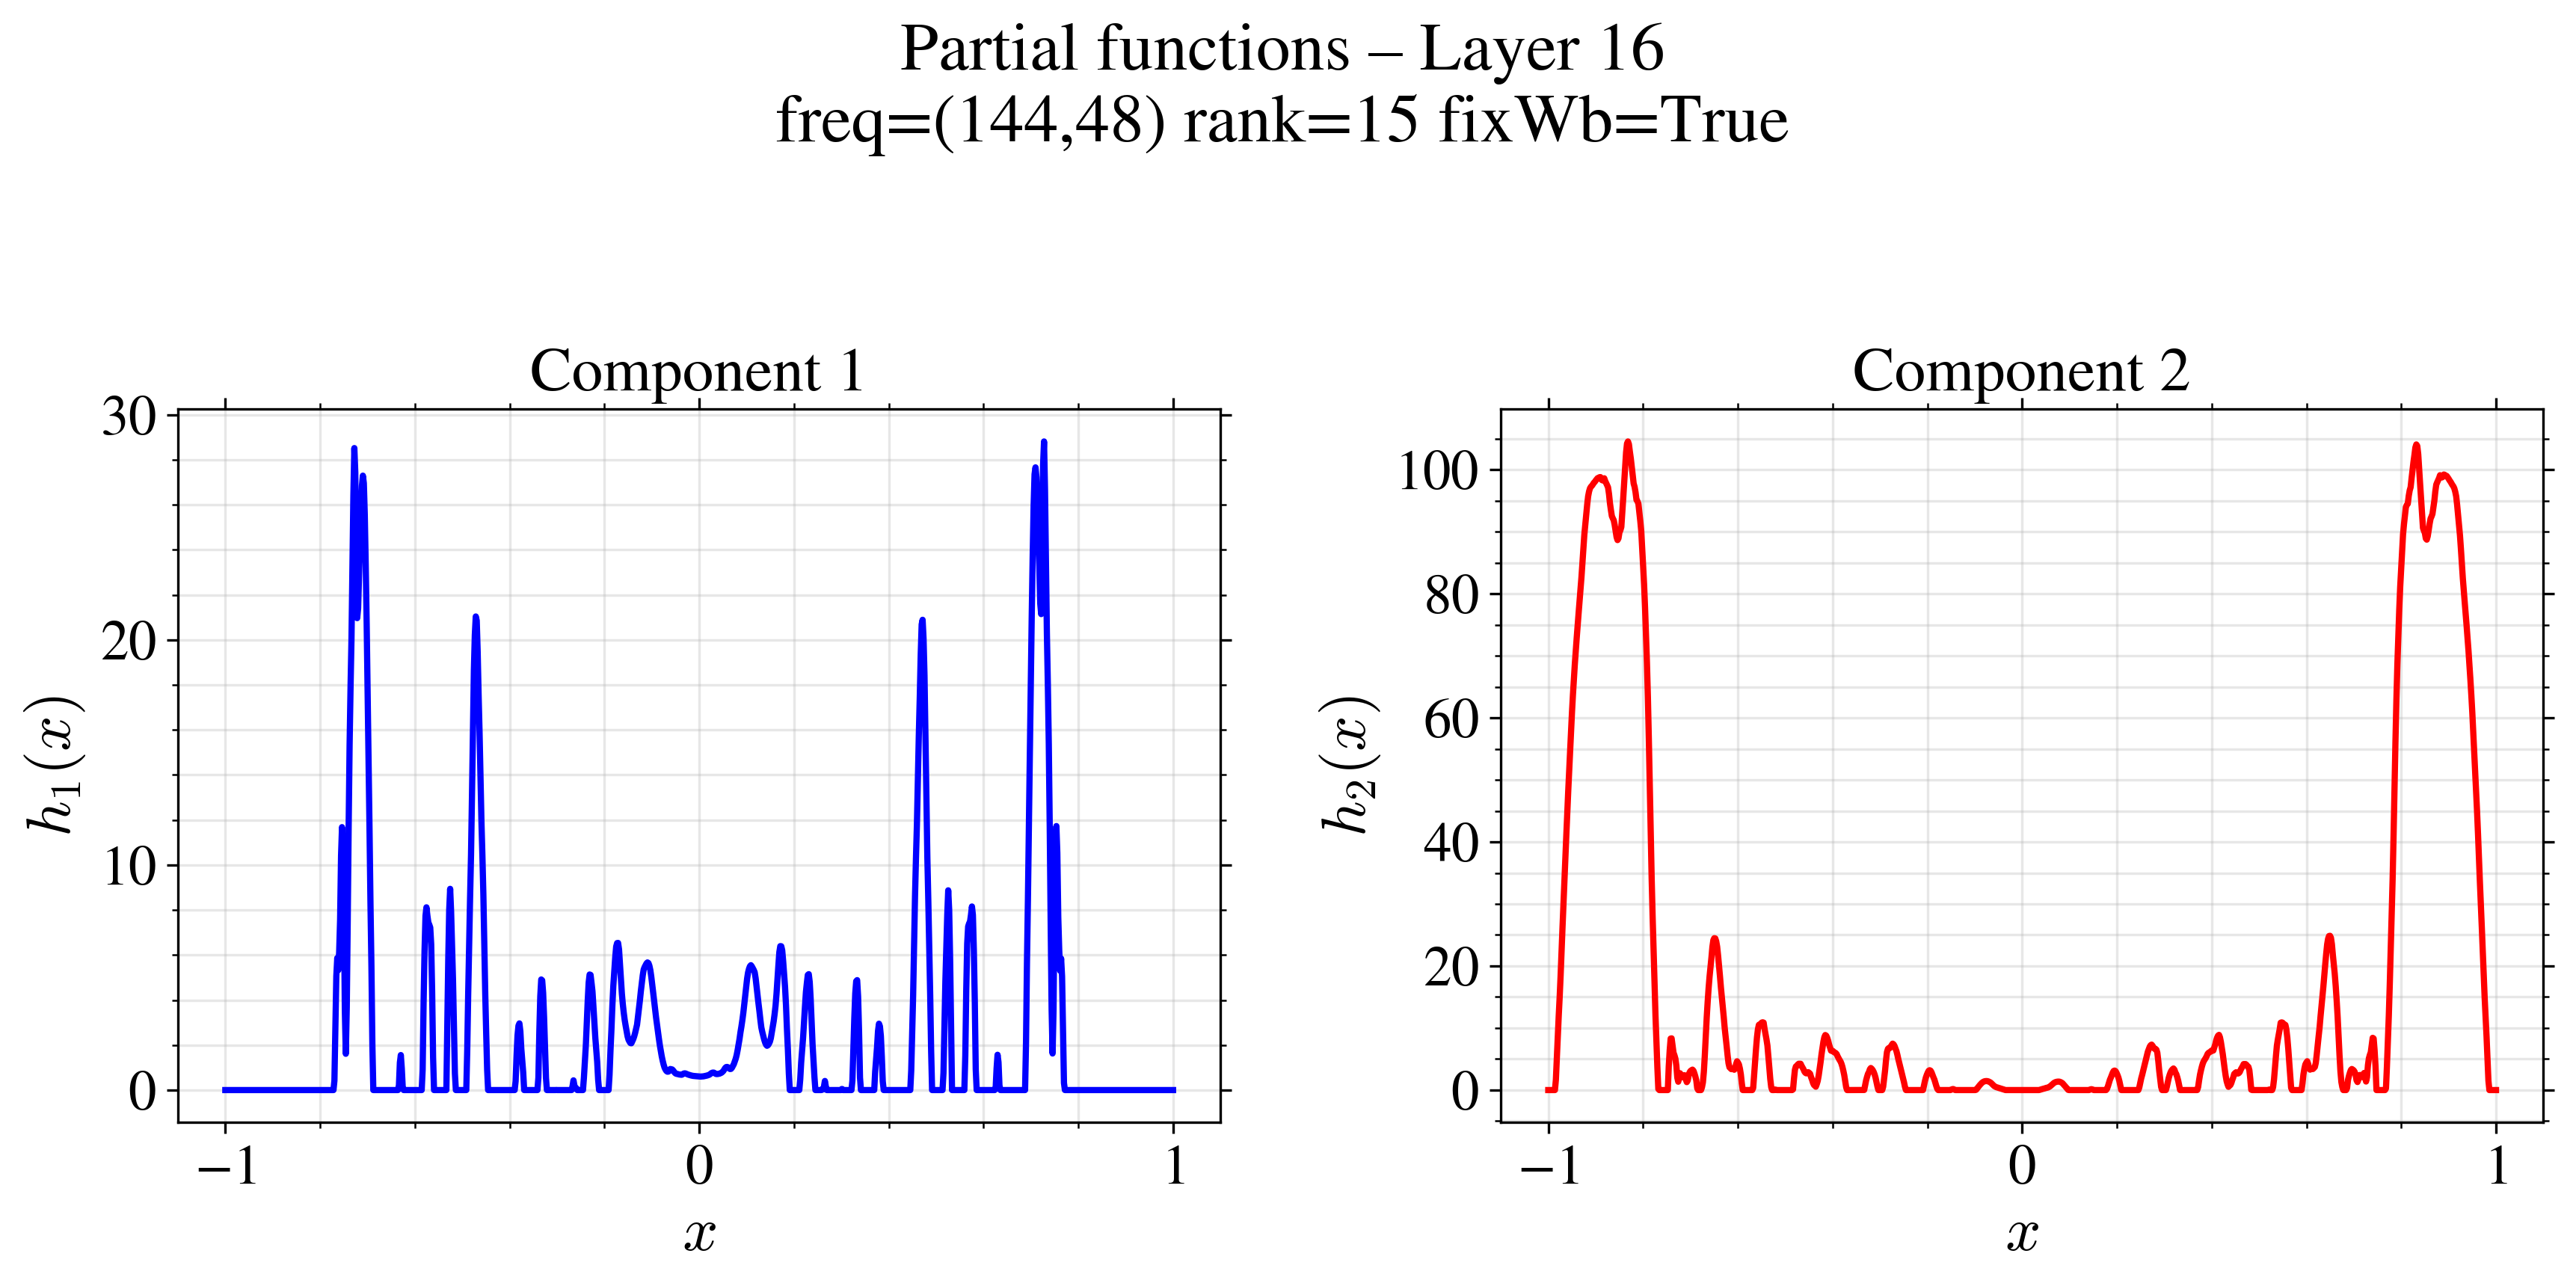
\includegraphics[width=\linewidth]{channel_partials_layer16.png}
    \end{column}
  \end{columns}
  \vspace{0.4em}
  \begin{itemize}
    \item Internal channels do not learn arbitrary shapes.
    \item They localize and sharpen useful patterns.
    \item Depth increases oscillation and hierarchy.
    \item The architecture organizes feature learning.
  \end{itemize}
\end{frame}

\begin{frame}{Low Rank Also Regularizes Geometry}
  \begin{columns}[T]
    \begin{column}{0.49\textwidth}
      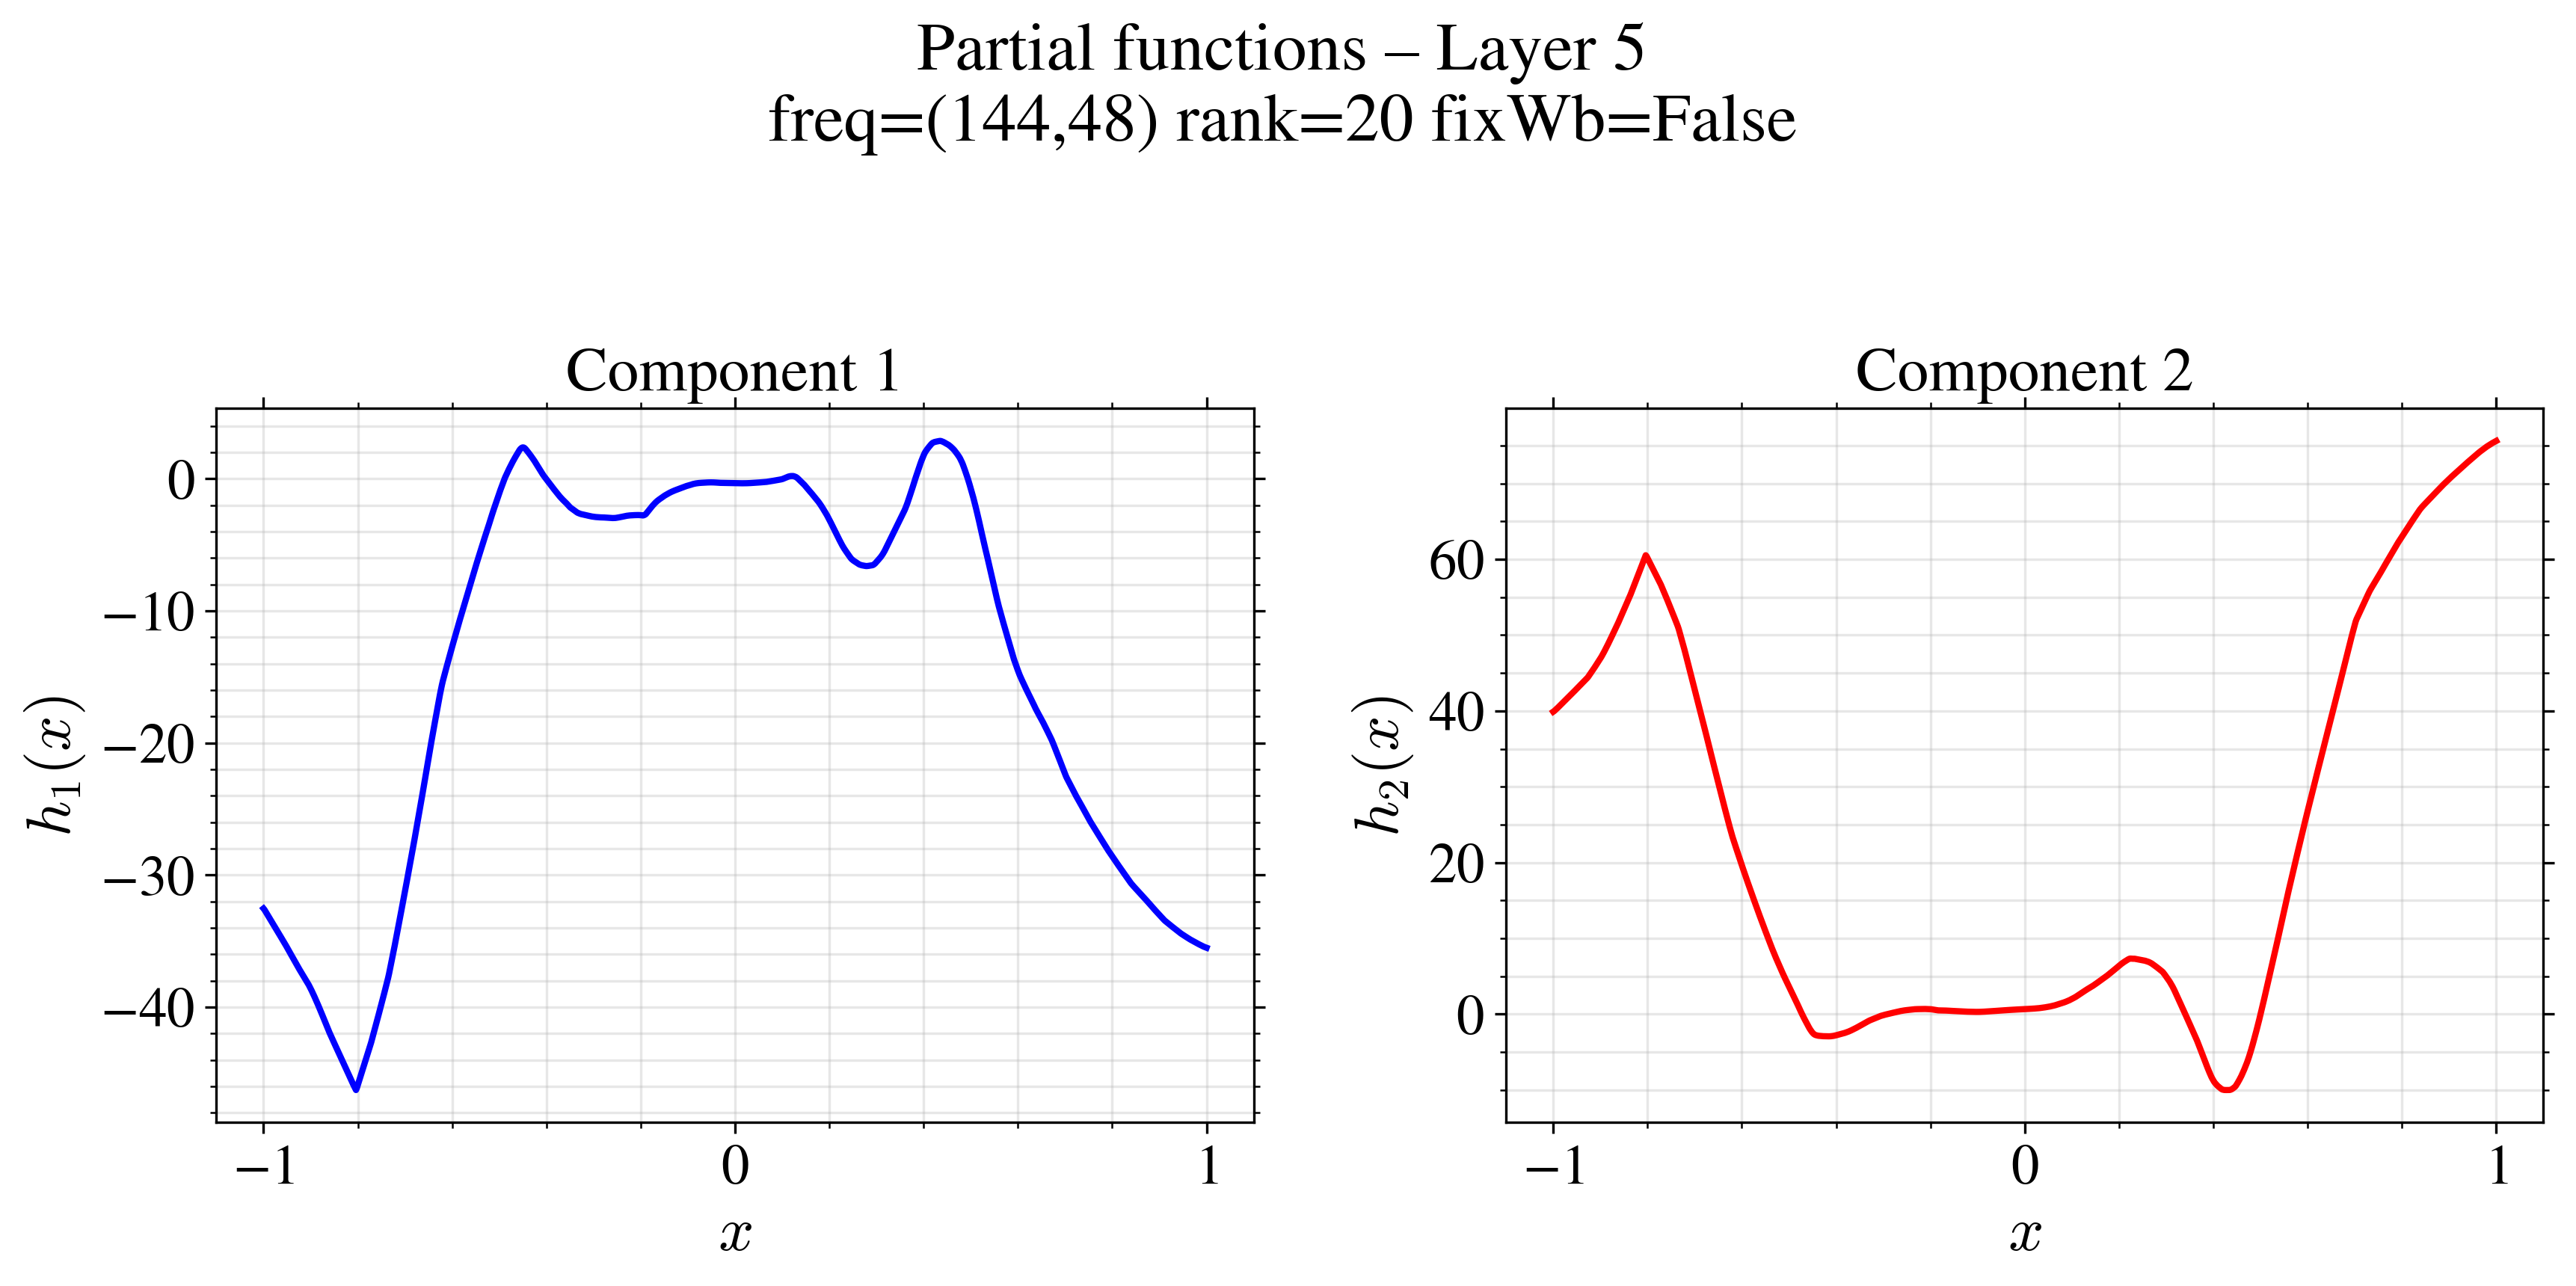
\includegraphics[width=\linewidth]{mlp_asymmetry_layer7.png}
    \end{column}
    \begin{column}{0.49\textwidth}
      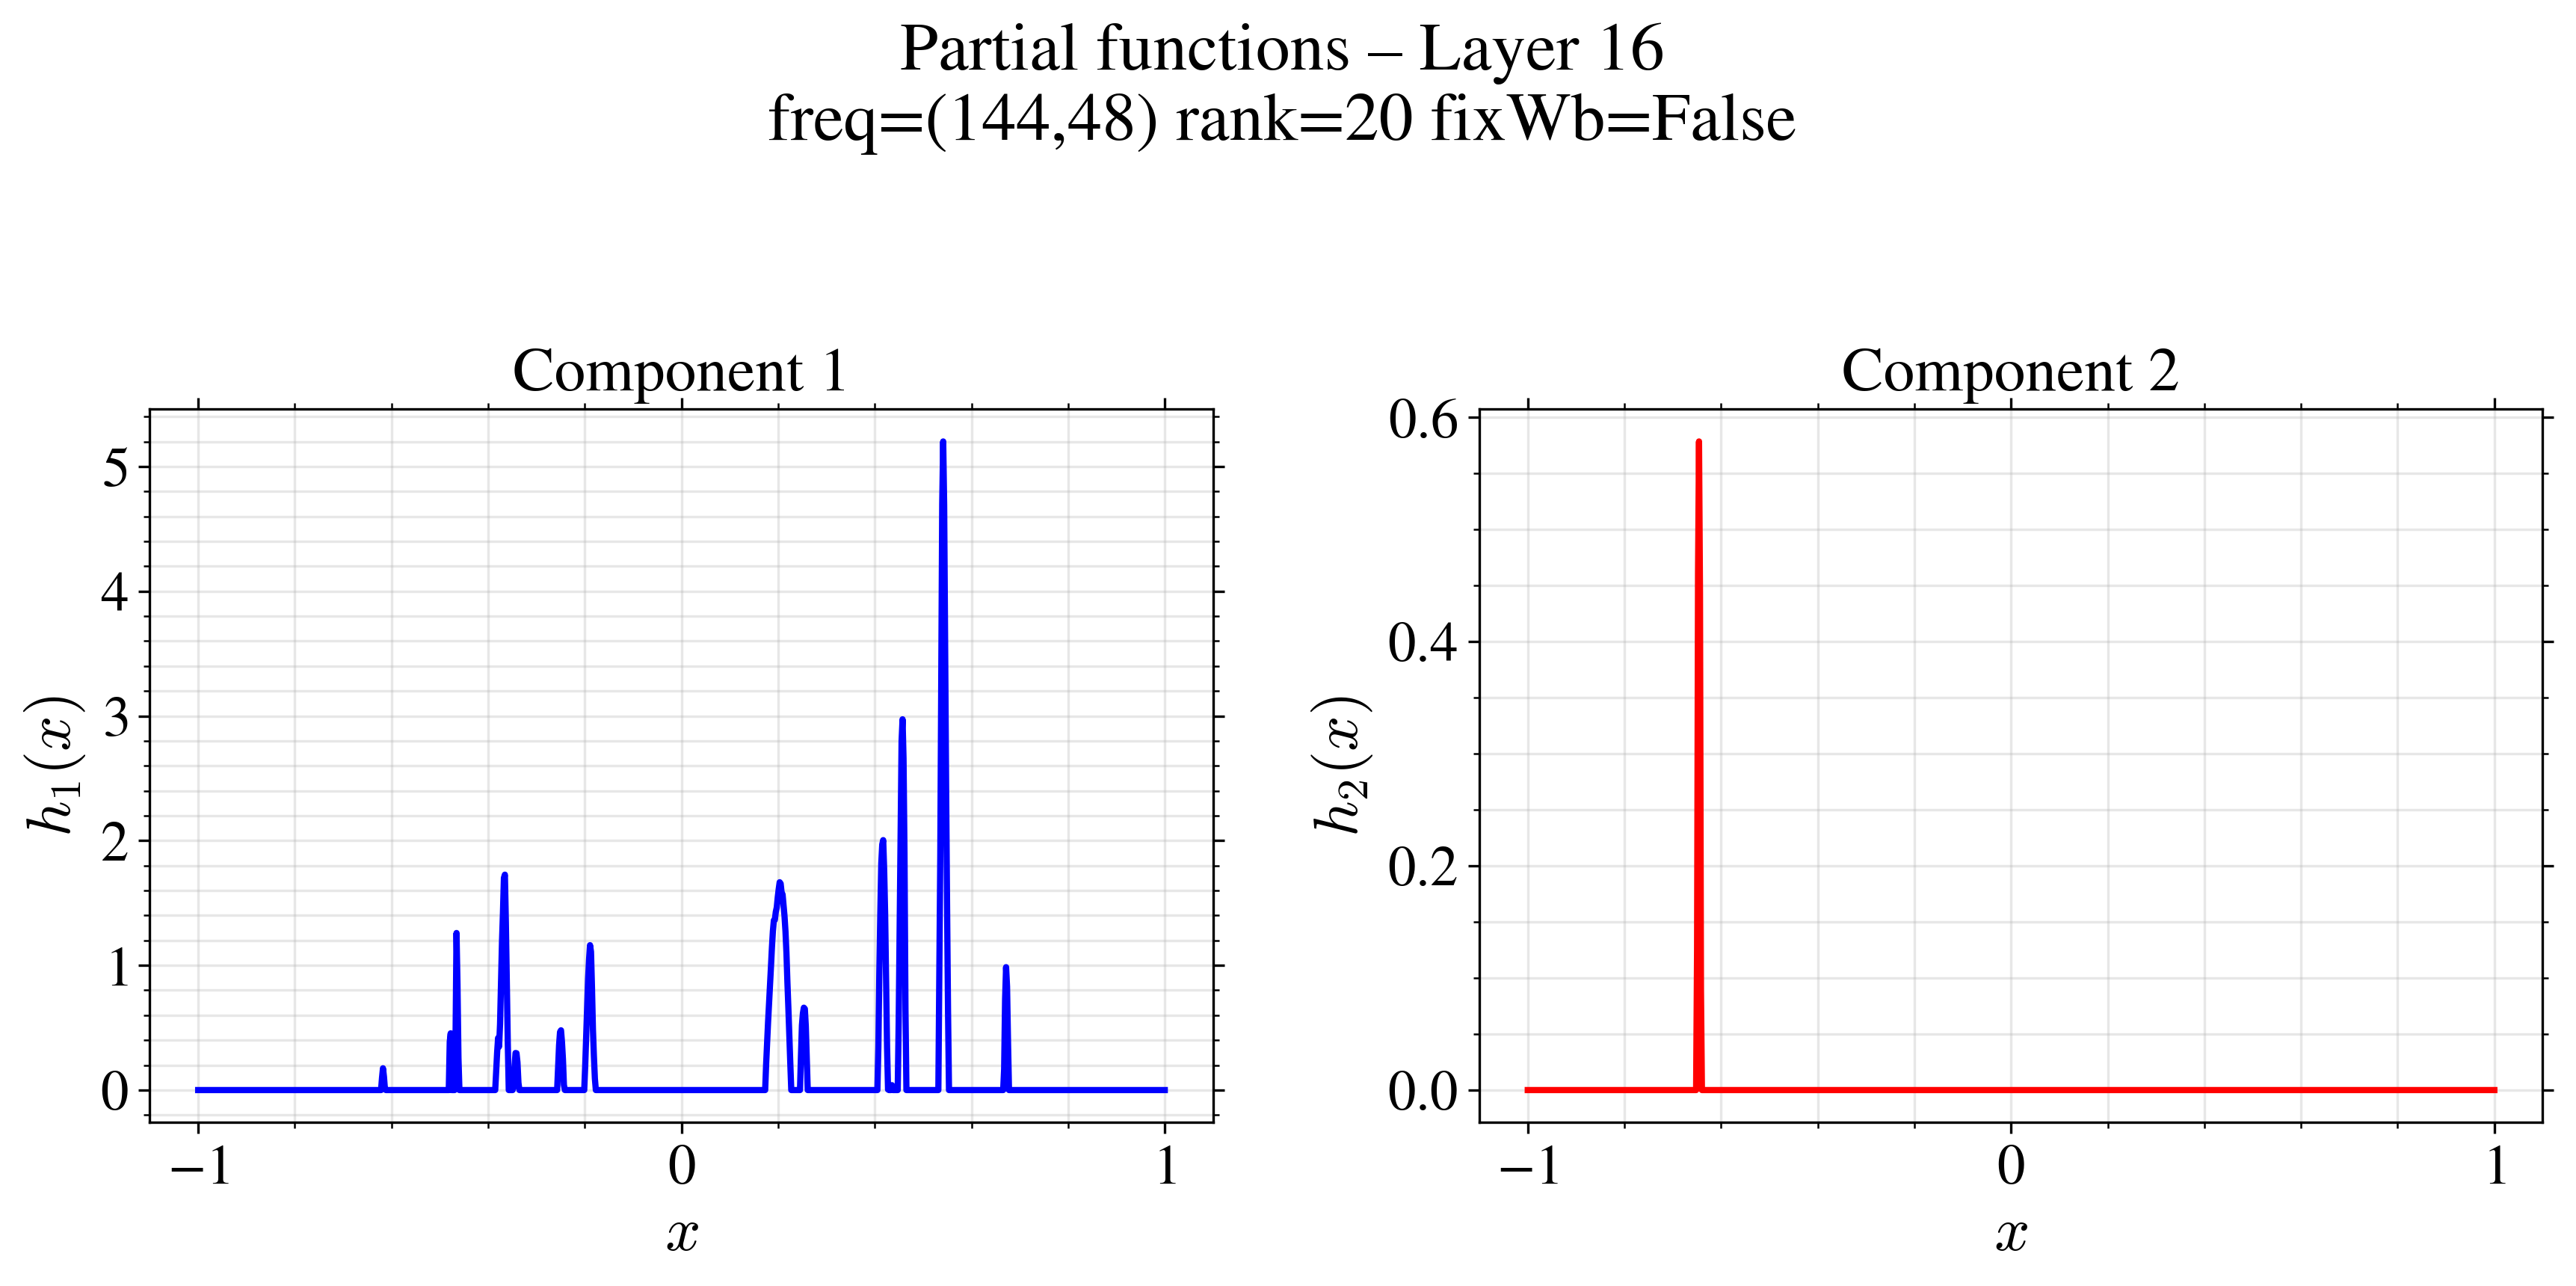
\includegraphics[width=\linewidth]{mlp_asymmetry_layer16.png}
    \end{column}
  \end{columns}
  \vspace{0.4em}
  \begin{itemize}
    \item Removing the low-rank structure degrades the internal geometry.
    \item Symmetry breaks more easily.
    \item Rank is not only a parameter-saving device.
    \item It also acts as a geometric regularizer.
  \end{itemize}
\end{frame}

\begin{frame}{Broader Perspective}
  \begin{block}{Theory}
    \begin{itemize}
      \item Architecture can be analyzed through explicit control parameters.
      \item Depth, rank, and geometry appear in closed-form statements.
    \end{itemize}
  \end{block}
  \begin{exampleblock}{Practice}
    \begin{itemize}
      \item The theoretical quantities are visible in numerical experiments.
    \end{itemize}
  \end{exampleblock}
  \begin{alertblock}{Program}
    \begin{itemize}
      \item This suggests a broader program for architecture-aware optimization.
    \end{itemize}
  \end{alertblock}
\end{frame}

\begin{frame}{Conclusion}
  \begin{block}{Takeaway 1}
    \begin{itemize}
      \item Deep optimization is hard. Architecture hits many levels at once.
    \end{itemize}
  \end{block}
  \begin{exampleblock}{Takeaway 2}
    \begin{itemize}
      \item Low rank: tractable model for those joint effects.
    \end{itemize}
  \end{exampleblock}
  \begin{alertblock}{Takeaway 3}
    \begin{itemize}
      \item Kernels, dynamics, experiments: one consistent story.
    \end{itemize}
  \end{alertblock}
\end{frame}

\appendix

\begin{frame}{Appendix: Additional Figure Gallery I}
  \begin{columns}[T]
    \begin{column}{0.49\textwidth}
      
\includegraphics[width=\linewidth,height=0.27\textheight,keepaspectratio]{confirm_prop17.png}
    \end{column}
    \begin{column}{0.49\textwidth}
      
\includegraphics[width=\linewidth,height=0.27\textheight,keepaspectratio]{decay_vs_depth.png}
    \end{column}
  \end{columns}
  \vspace{0.4em}
  \begin{columns}[T]
    \begin{column}{0.49\textwidth}
      
\includegraphics[width=\linewidth,height=0.27\textheight,keepaspectratio]{variance_vs_r.png}
    \end{column}
    \begin{column}{0.49\textwidth}
      
\includegraphics[width=\linewidth,height=0.27\textheight,keepaspectratio]{min_eig_distribution.png}
    \end{column}
  \end{columns}
\end{frame}

\begin{frame}{Appendix: Additional Figure Gallery II}
  \begin{columns}[T]
    \begin{column}{0.49\textwidth}
      
\includegraphics[width=\linewidth,height=0.27\textheight,keepaspectratio]{min_eig_mean_vs_r.png}
    \end{column}
    \begin{column}{0.49\textwidth}
      
\includegraphics[width=\linewidth,height=0.27\textheight,keepaspectratio]{condition_number_proxy_vs_empirical.png}
    \end{column}
  \end{columns}
  \vspace{0.4em}
  \begin{columns}[T]
    \begin{column}{0.49\textwidth}
      
\includegraphics[width=\linewidth,height=0.27\textheight,keepaspectratio]{condition_number_highdim_spherical.png}
    \end{column}
    \begin{column}{0.49\textwidth}
      
\includegraphics[width=\linewidth,height=0.27\textheight,keepaspectratio]{kernel_regression_risk_vs_r.png}
    \end{column}
  \end{columns}
\end{frame}

\begin{frame}{Appendix: MMNN NTK Gallery I}
  \begin{columns}[T]
    \begin{column}{0.49\textwidth}
      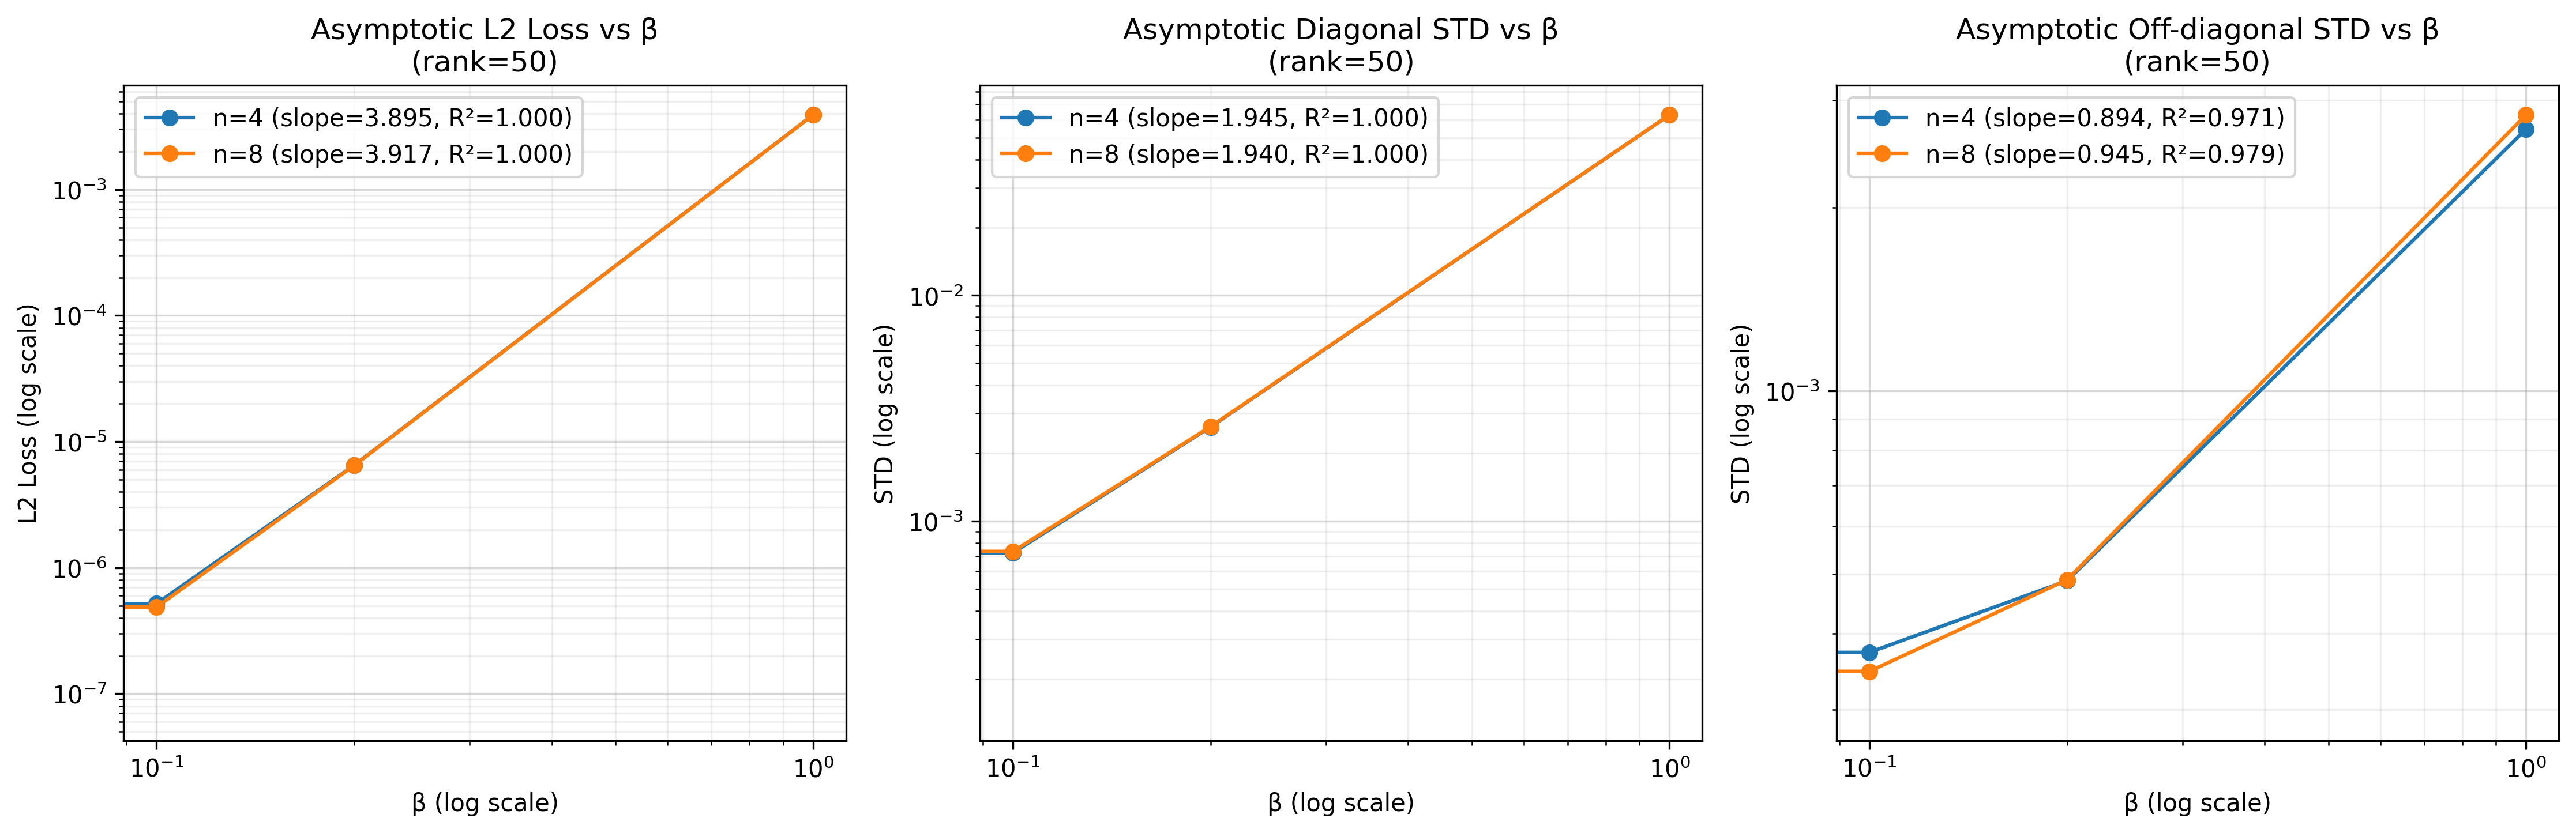
\includegraphics[width=\linewidth,height=0.27\textheight,keepaspectratio]{convergence_vs_beta_rank50.png}
    \end{column}
    \begin{column}{0.49\textwidth}
      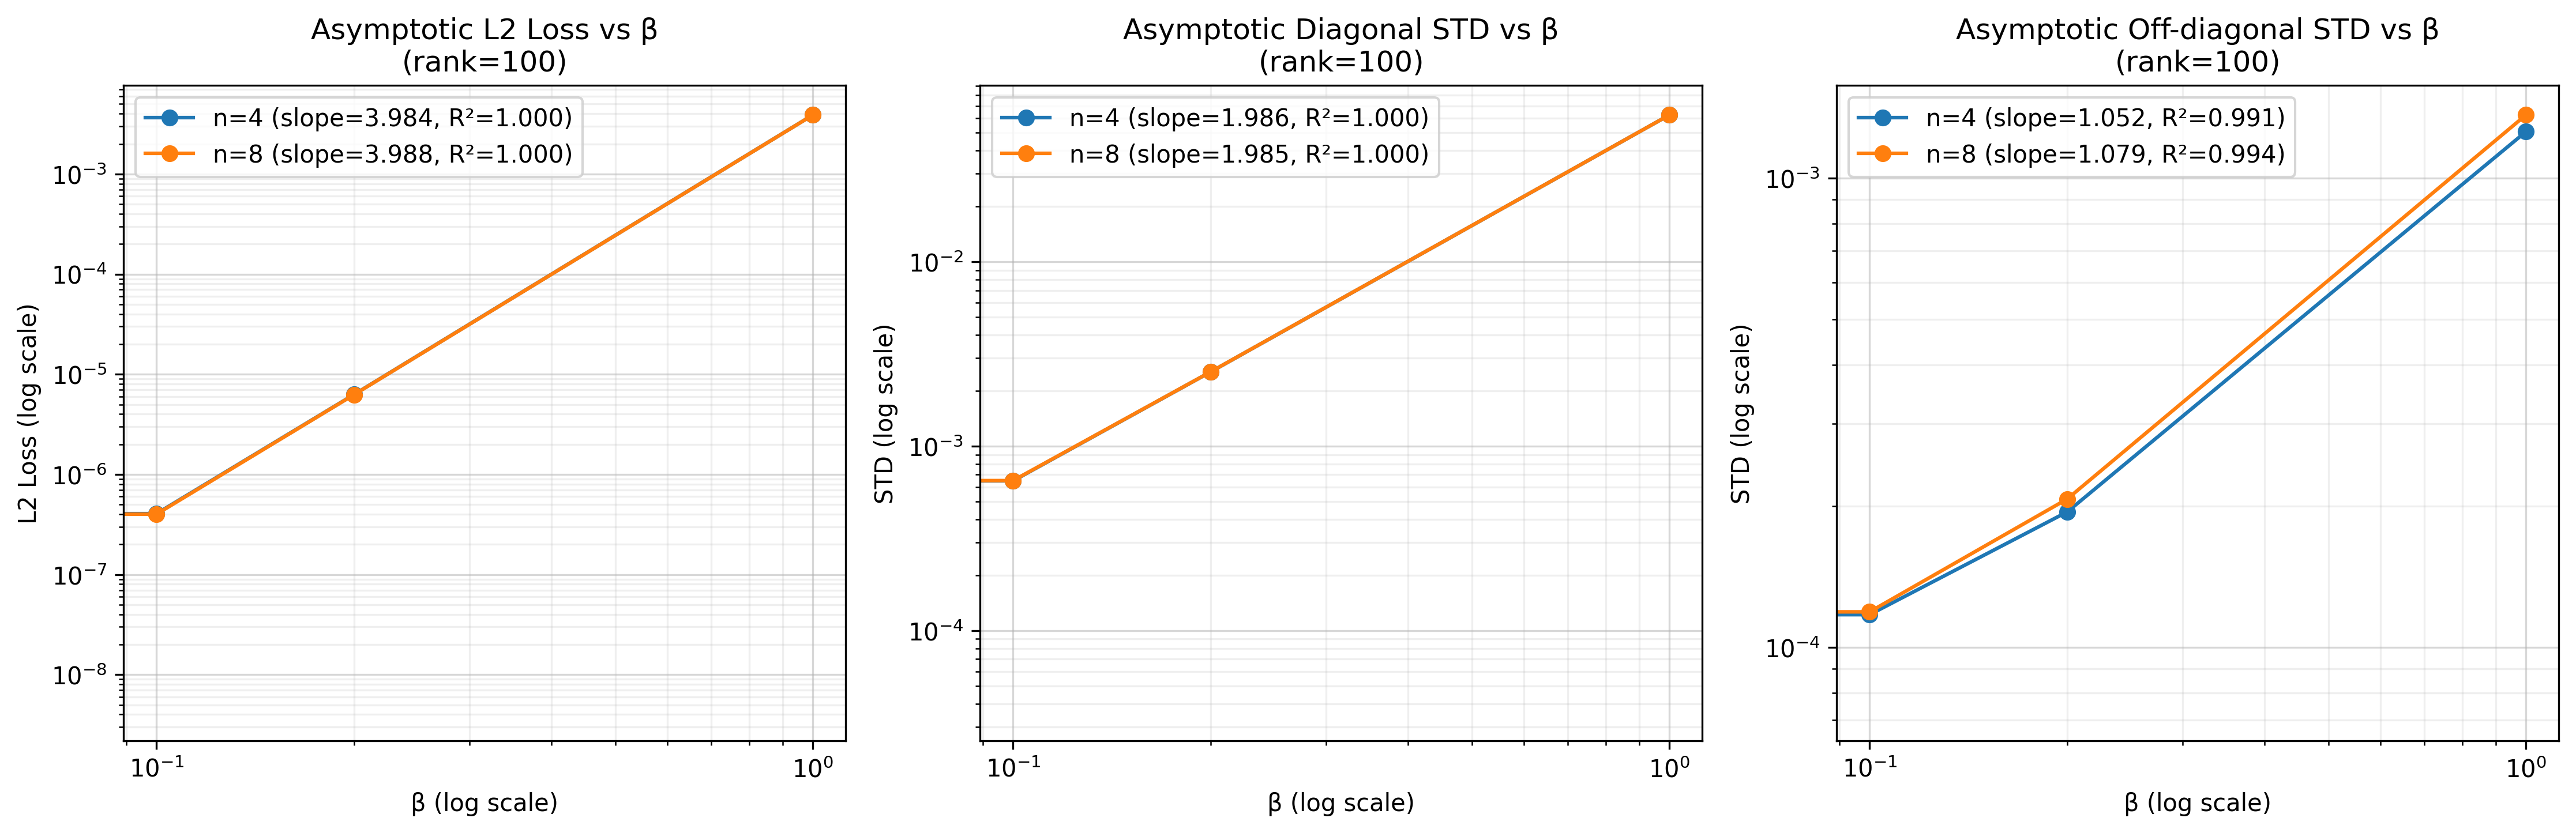
\includegraphics[width=\linewidth,height=0.27\textheight,keepaspectratio]{convergence_vs_beta_rank100.png}
    \end{column}
  \end{columns}
  \vspace{0.4em}
  \begin{columns}[T]
    \begin{column}{0.49\textwidth}
      
\includegraphics[width=\linewidth,height=0.27\textheight,keepaspectratio]{ntk_distributions_rank2_beta1.0_gaussian.png}
    \end{column}
    \begin{column}{0.49\textwidth}
      
\includegraphics[width=\linewidth,height=0.27\textheight,keepaspectratio]{ntk_distributions_rank5_beta1.0_gaussian.png}
    \end{column}
  \end{columns}
\end{frame}

\begin{frame}{Appendix: MMNN NTK Gallery II}
  \begin{columns}[T]
    \begin{column}{0.49\textwidth}
      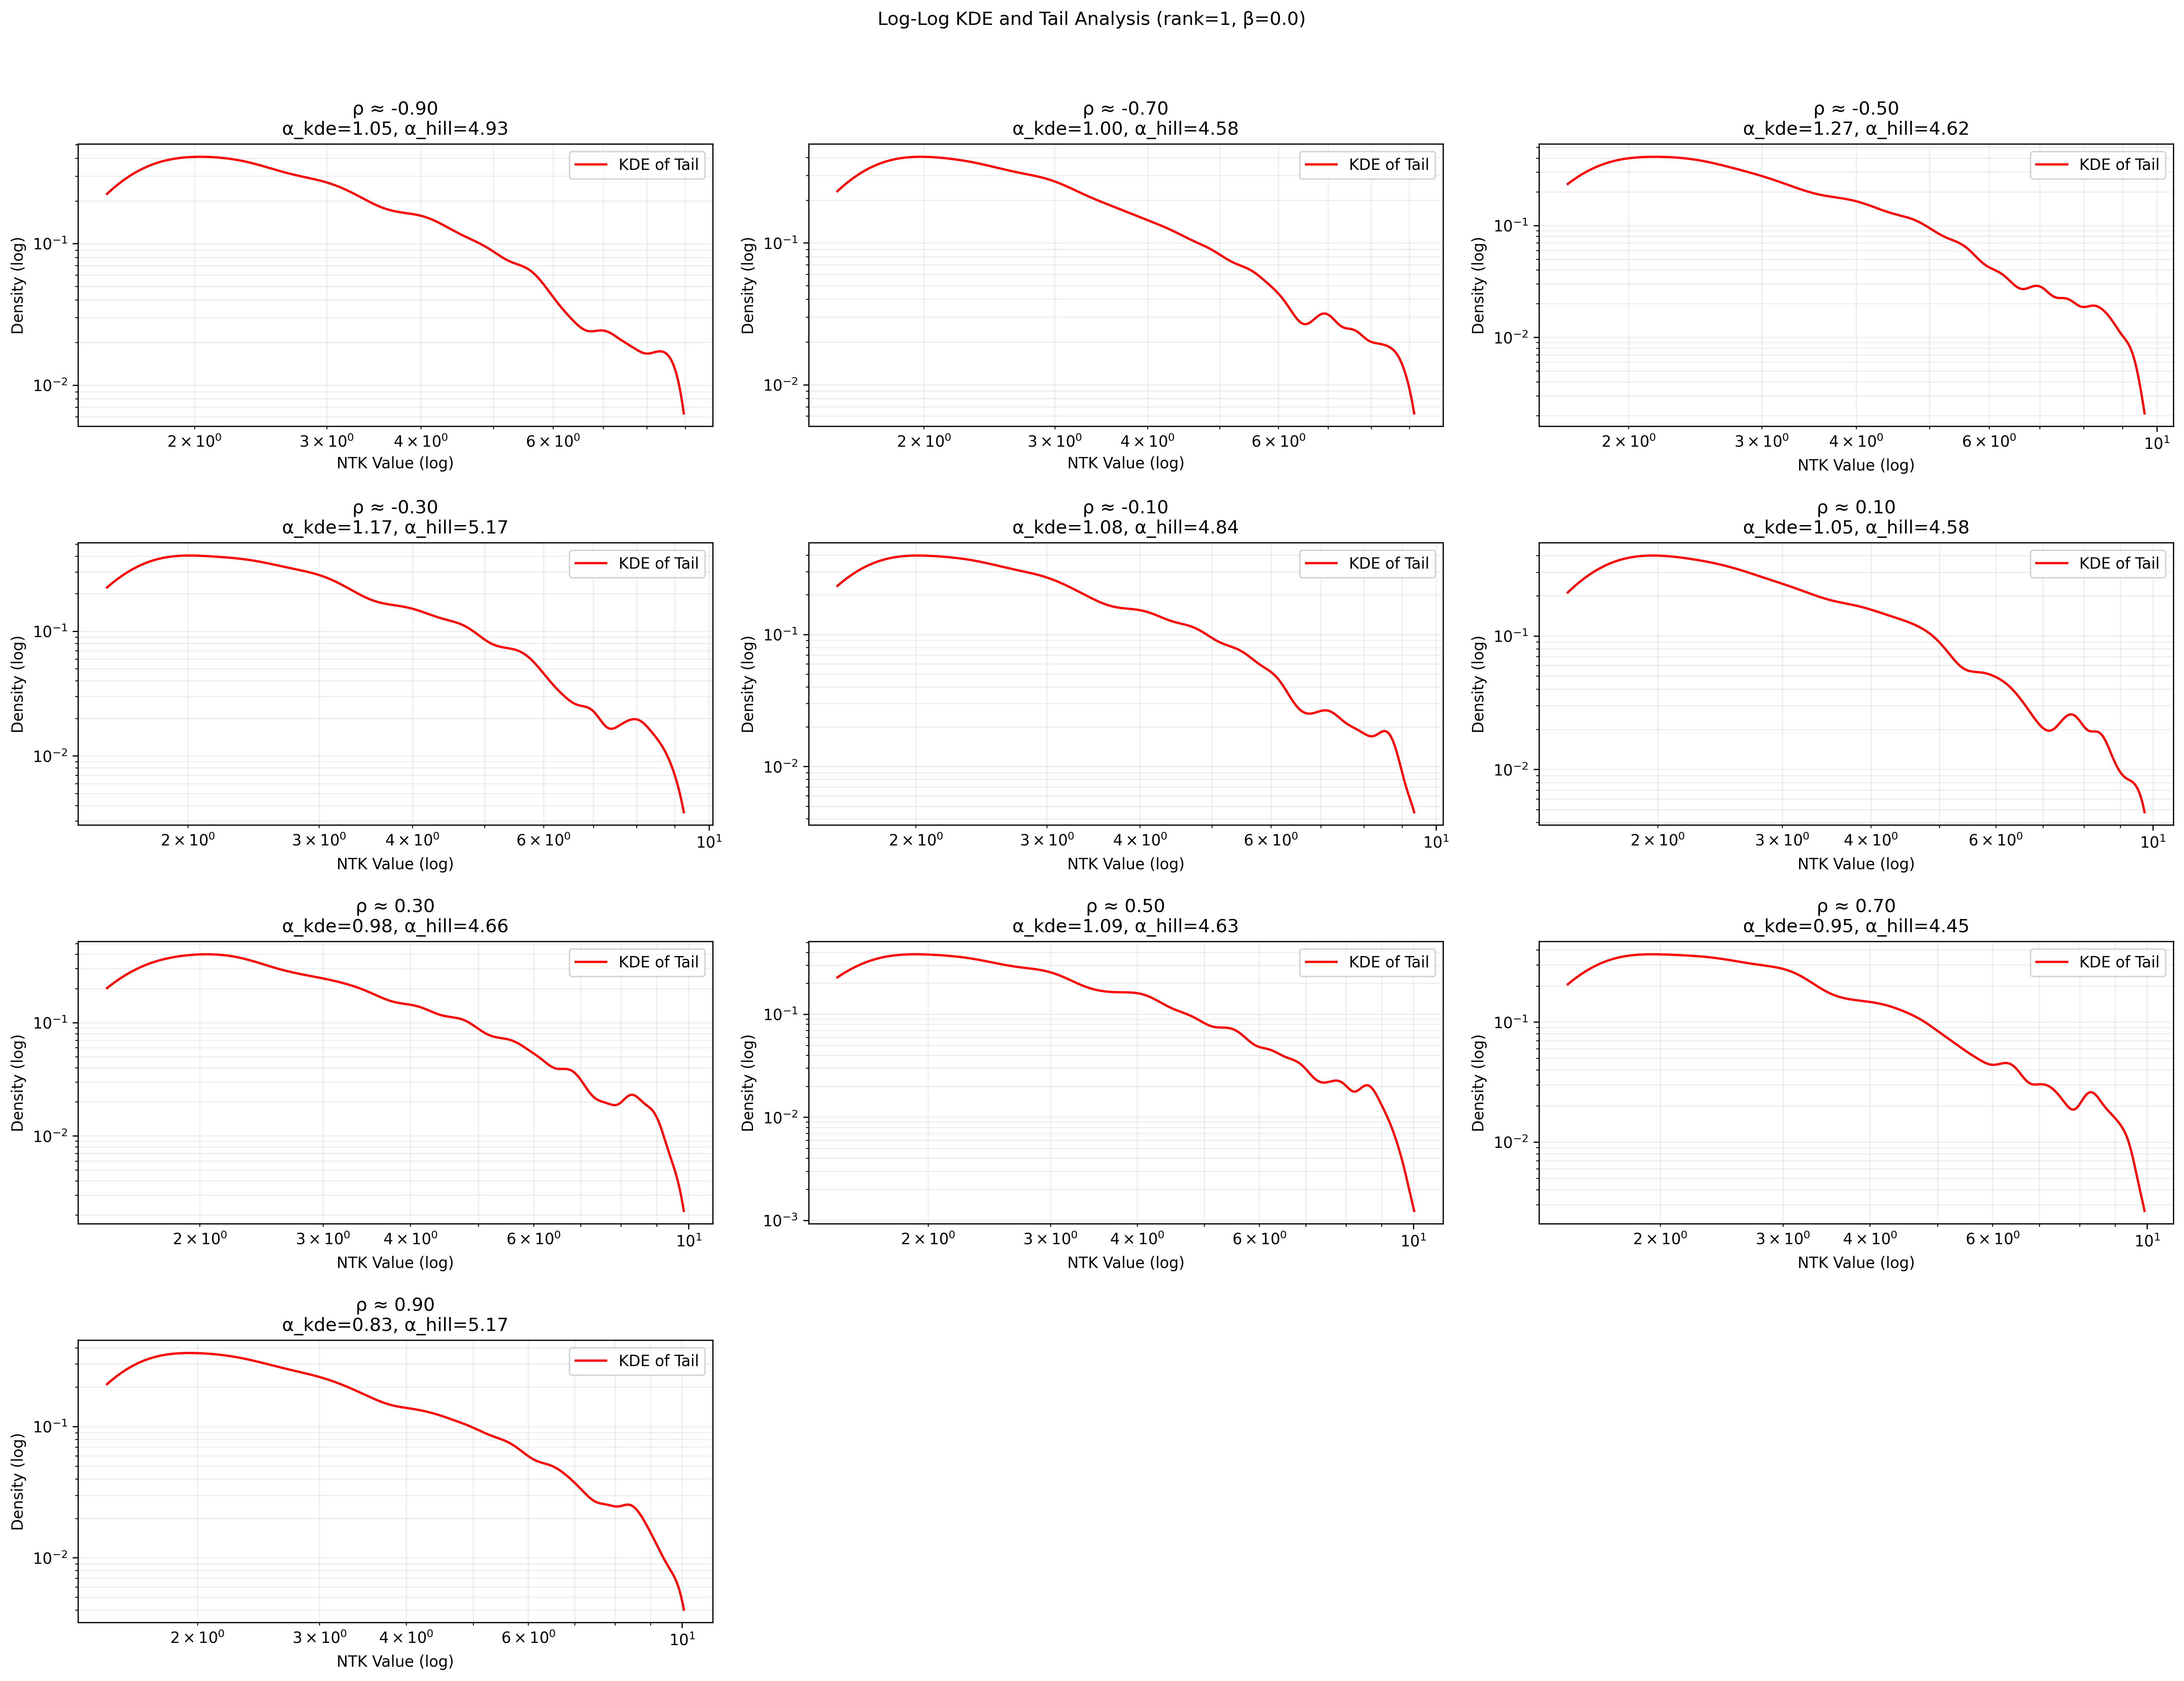
\includegraphics[width=\linewidth,height=0.27\textheight,keepaspectratio]{ntk_loglog_kde_rank1_beta0.0_gaussian.png}
    \end{column}
    \begin{column}{0.49\textwidth}
      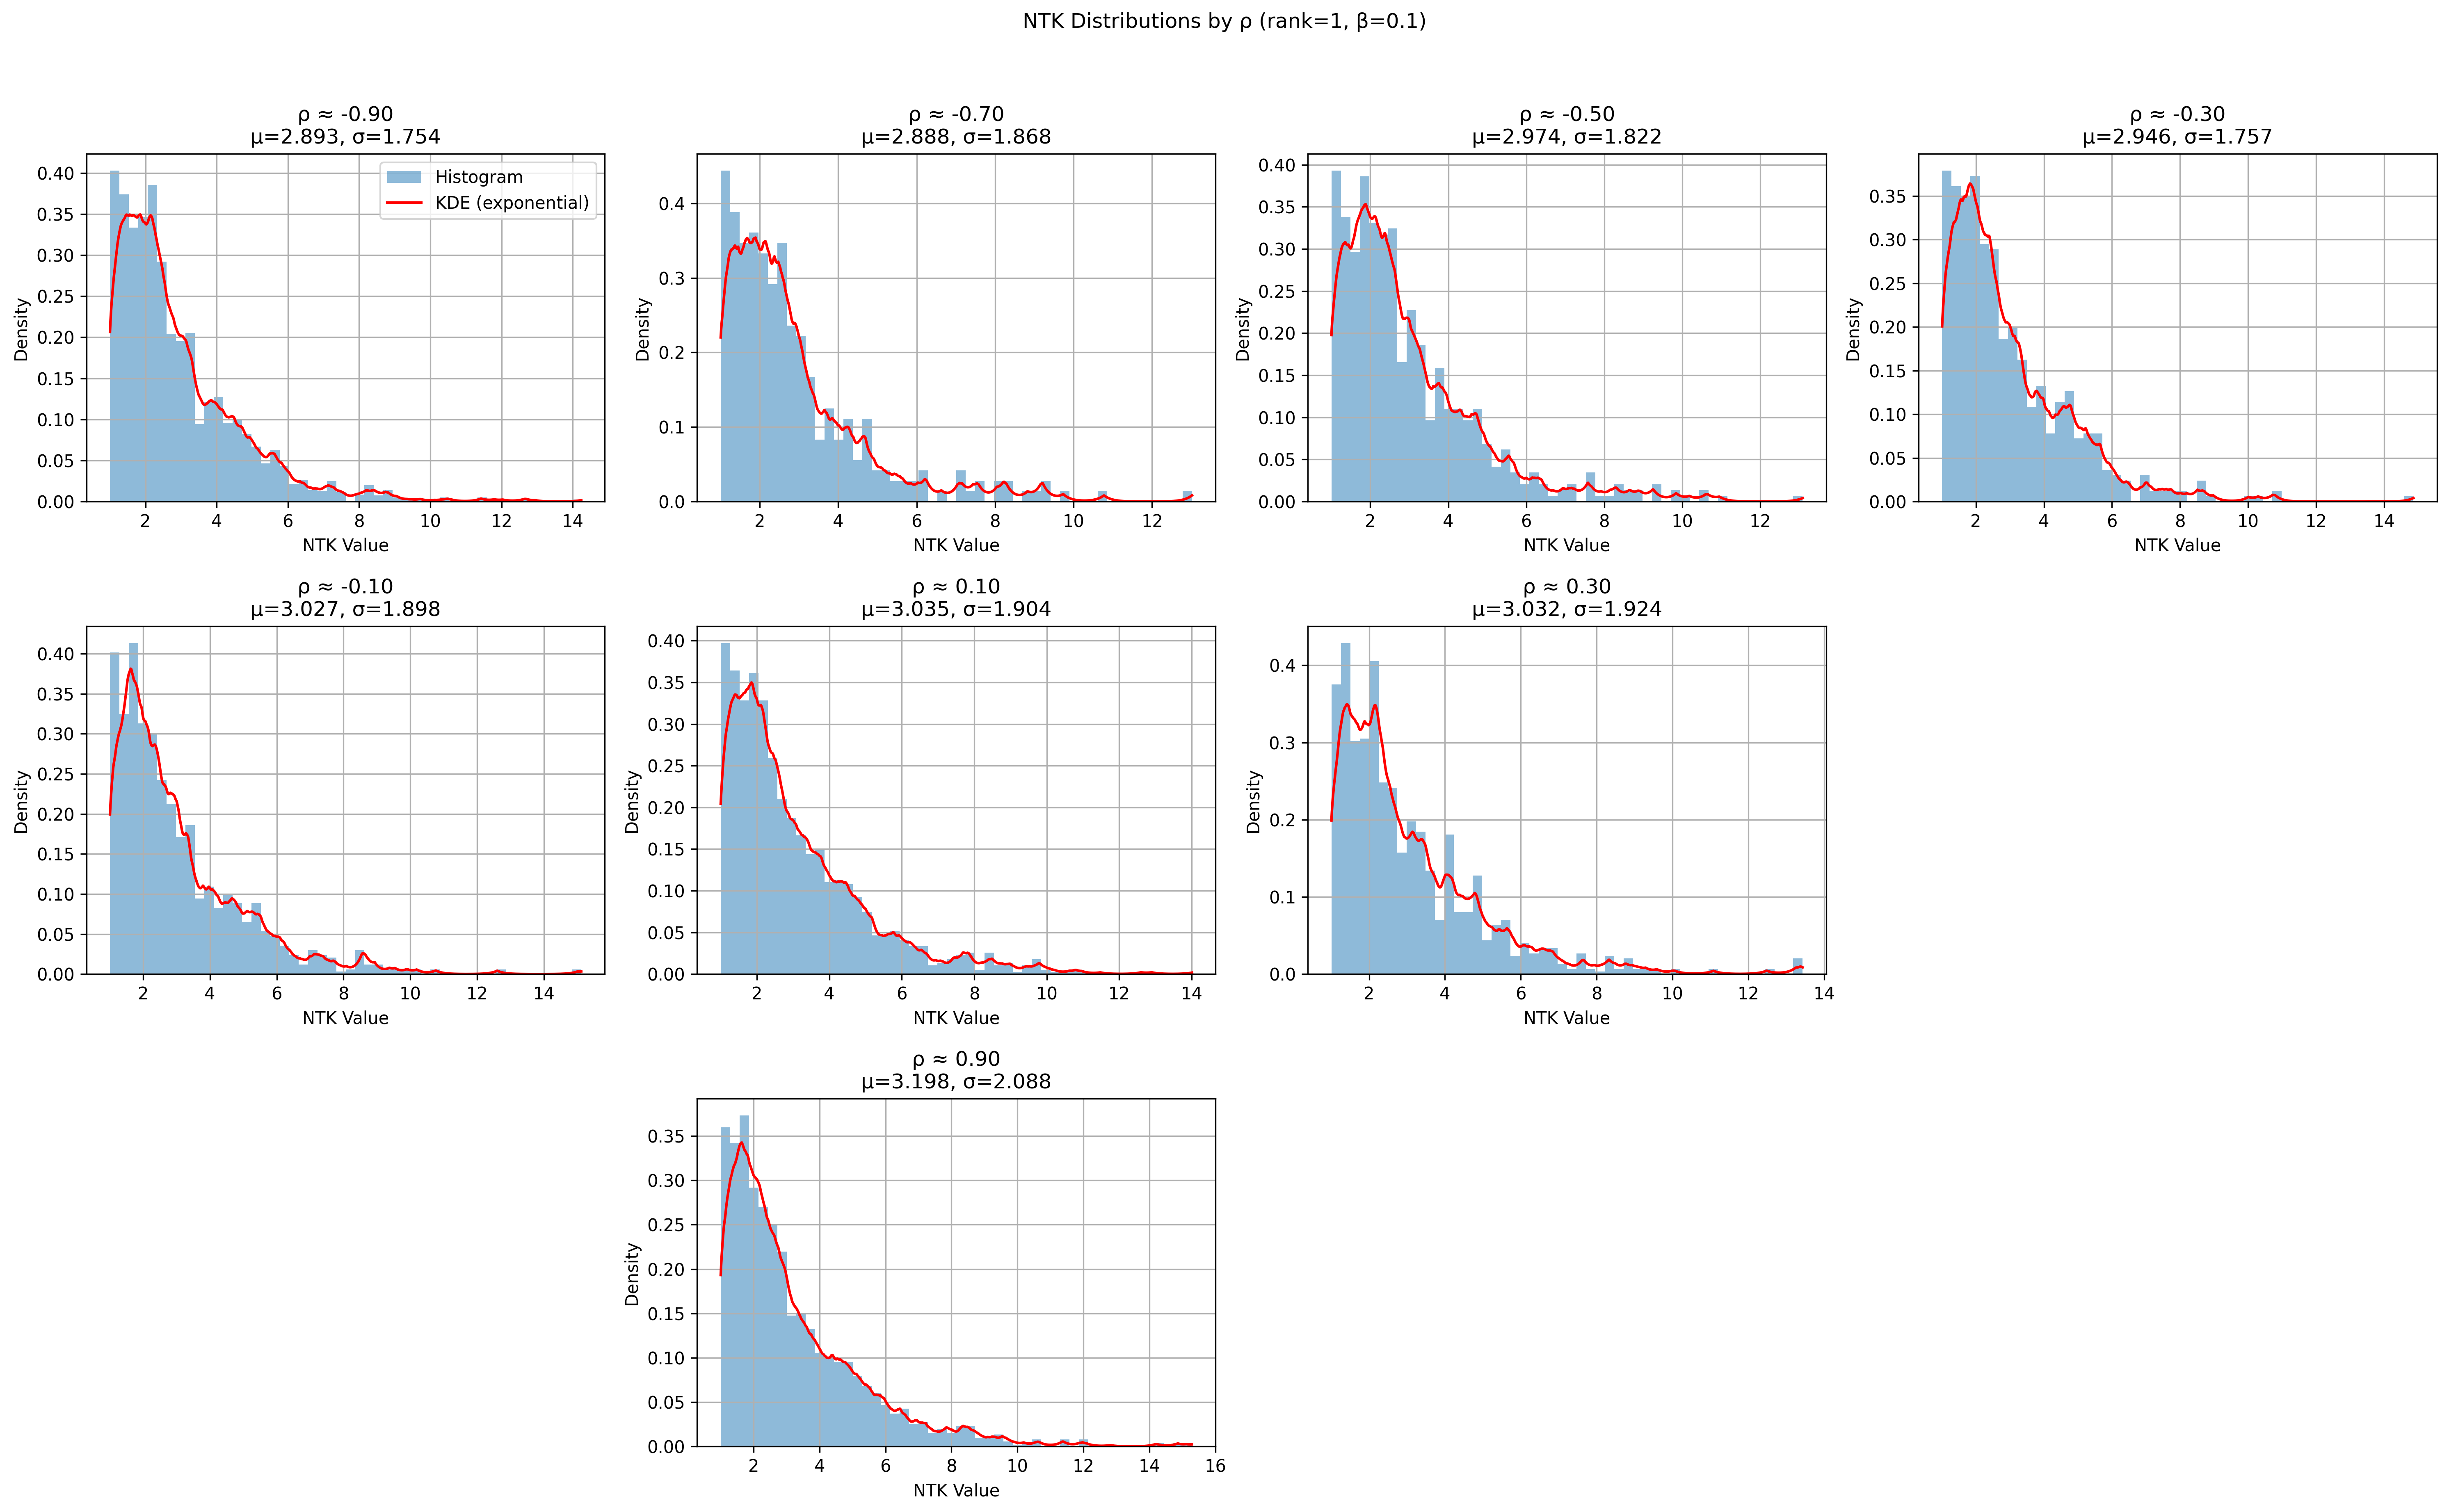
\includegraphics[width=\linewidth,height=0.27\textheight,keepaspectratio]{ntk_distributions_by_rho_rank1_beta0.1_exponential_bw0.2.png}
    \end{column}
  \end{columns}
  \vspace{0.4em}
  \begin{columns}[T]
    \begin{column}{0.49\textwidth}
      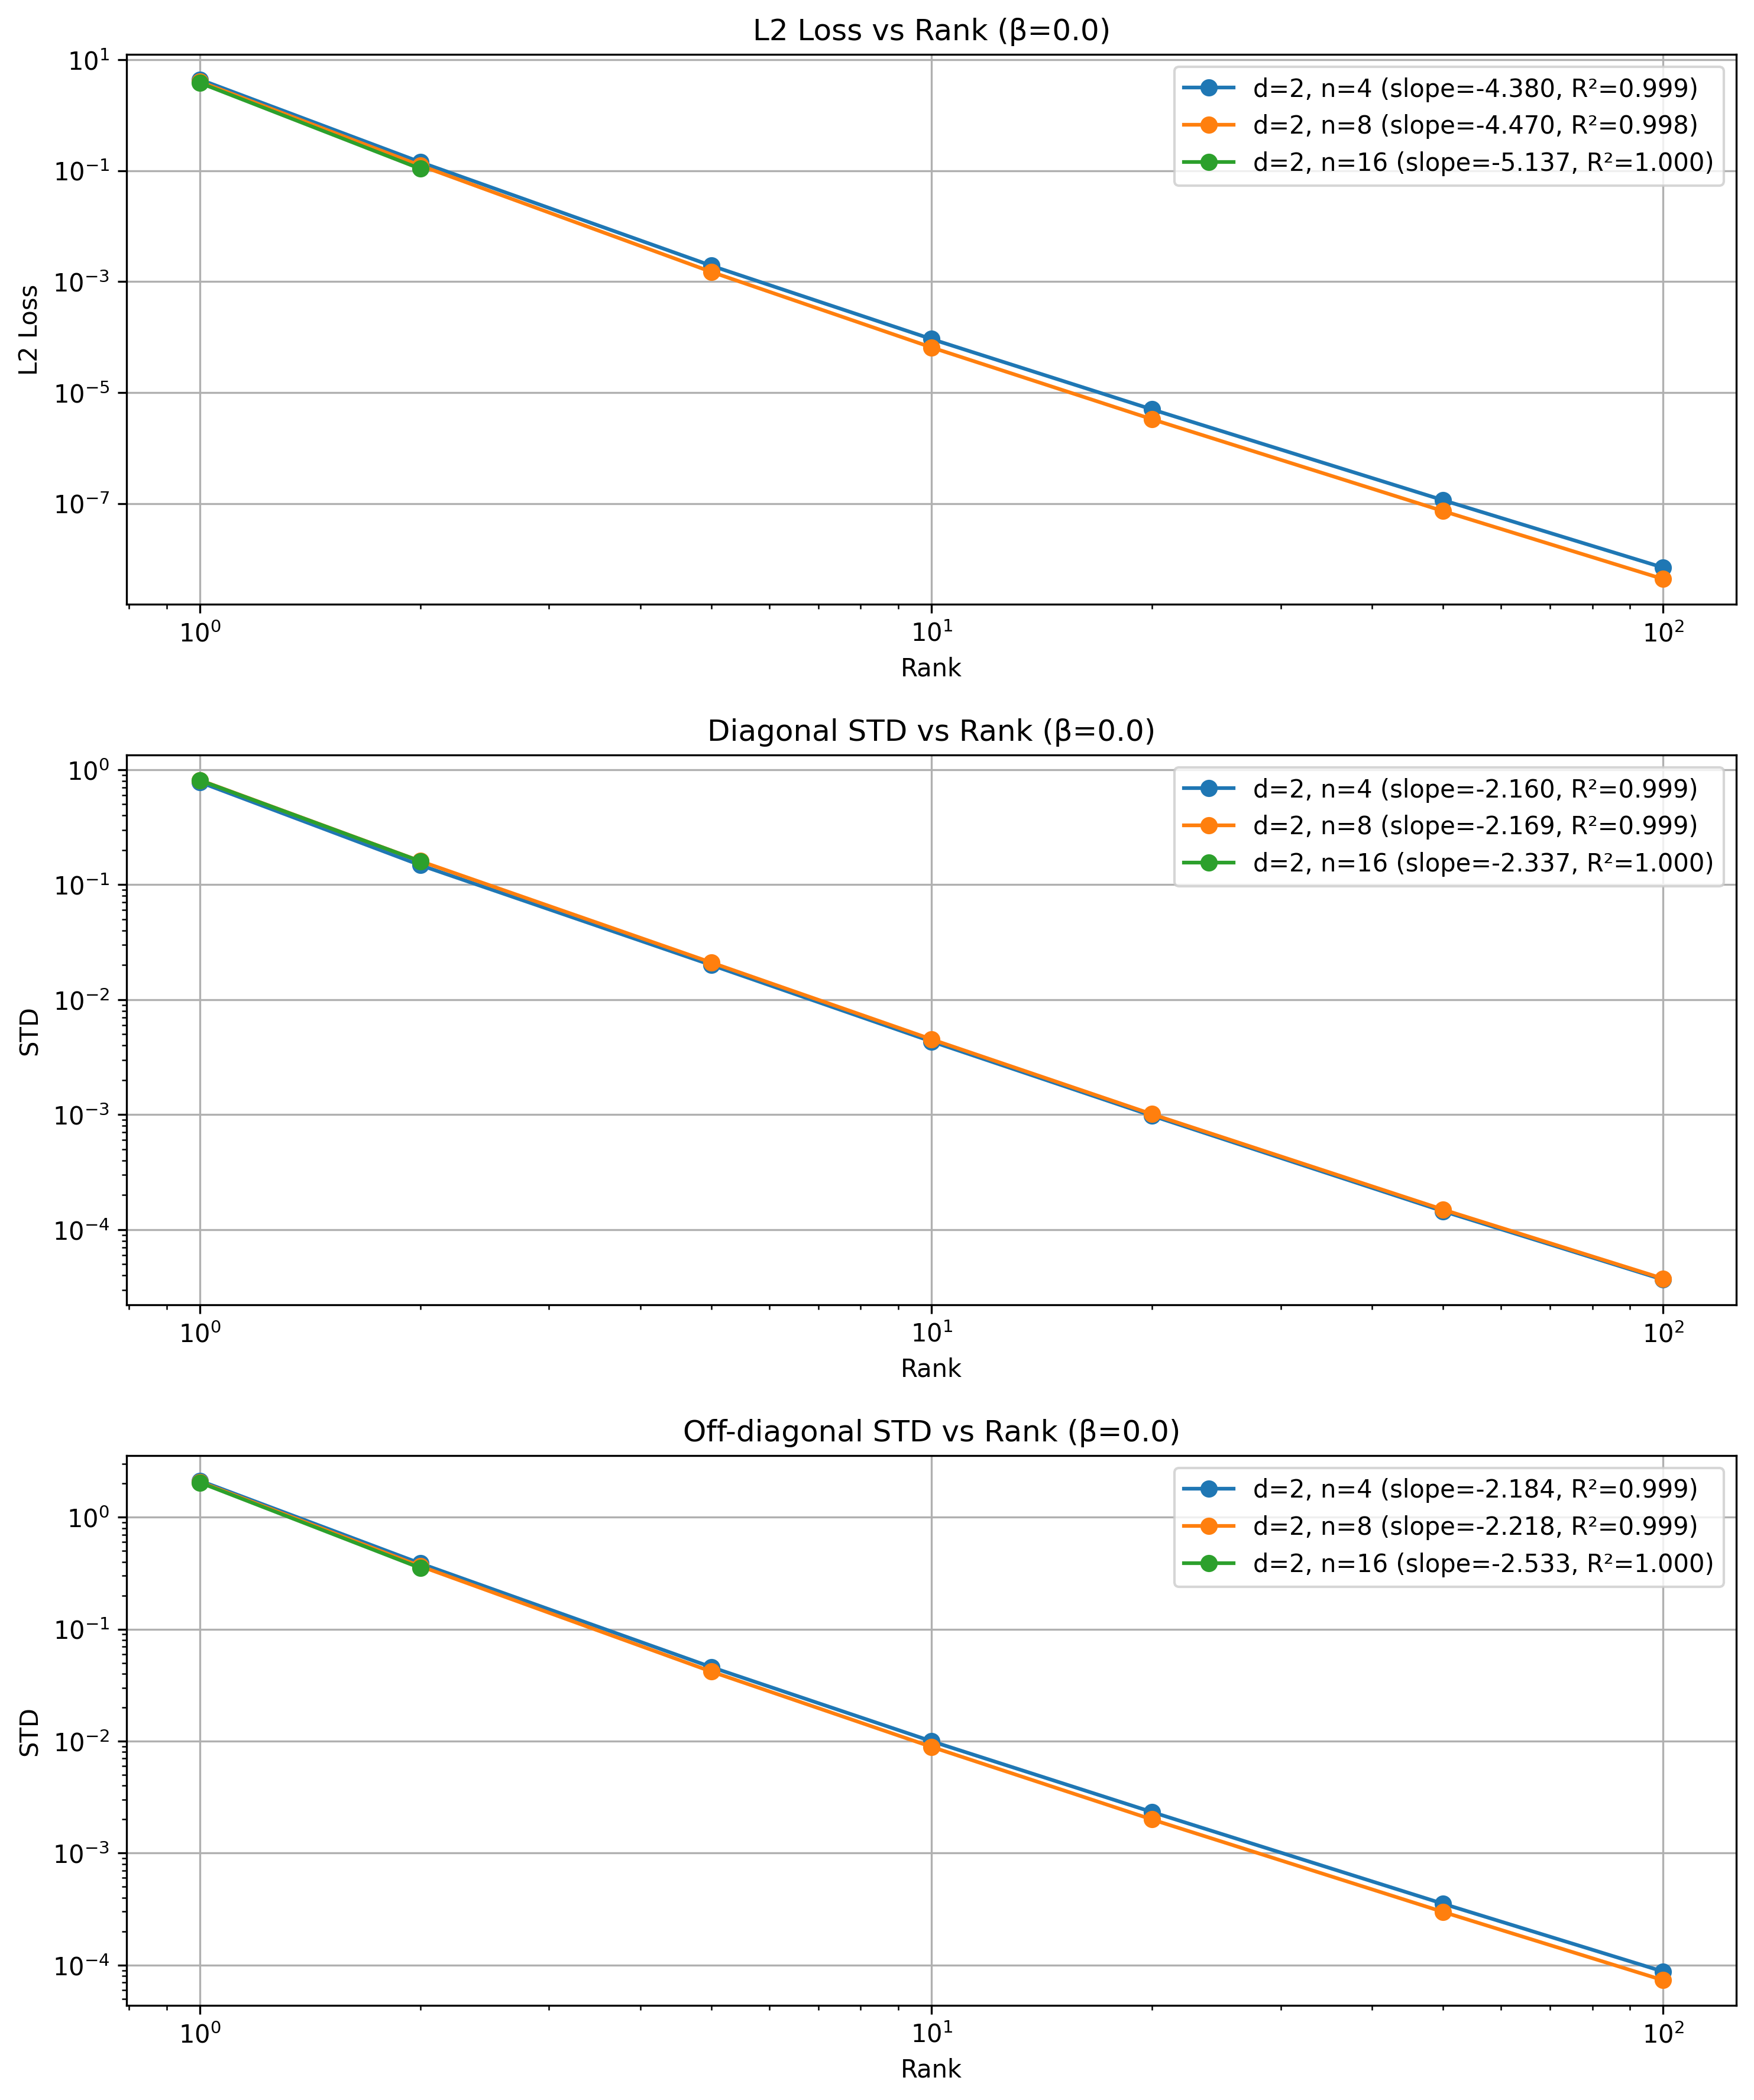
\includegraphics[width=\linewidth,height=0.27\textheight,keepaspectratio]{rank_scaling_beta0.png}
    \end{column}
    \begin{column}{0.49\textwidth}
      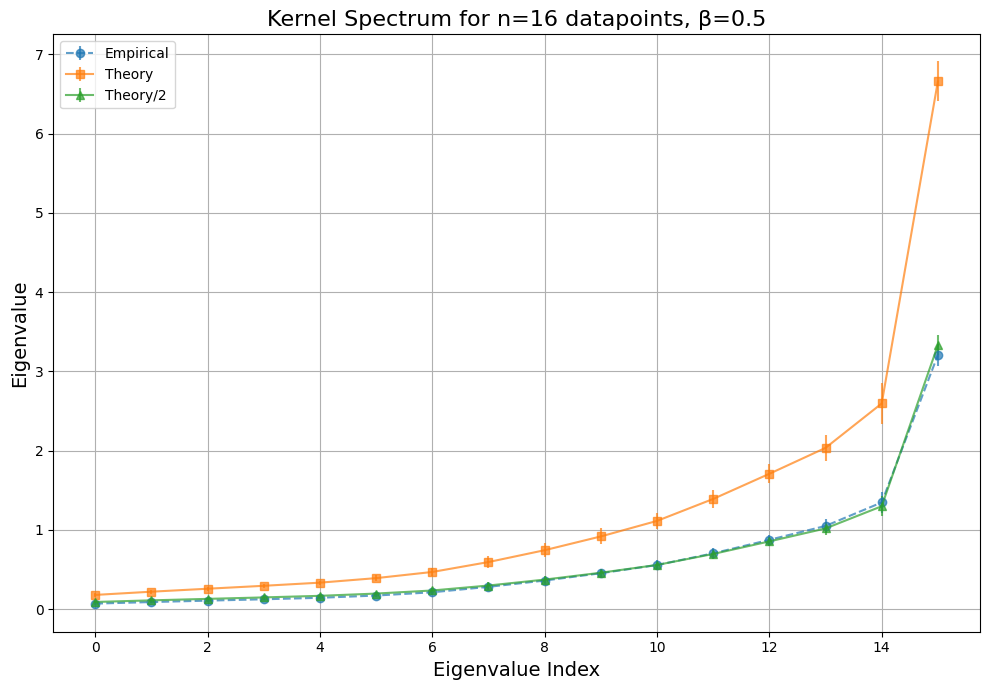
\includegraphics[width=\linewidth,height=0.27\textheight,keepaspectratio]{kernelspectrum_mlp_mmnn.png}
    \end{column}
  \end{columns}
\end{frame}

\begin{frame}{Appendix: Feature-Learning Gallery I}
  \begin{columns}[T]
    \begin{column}{0.49\textwidth}
      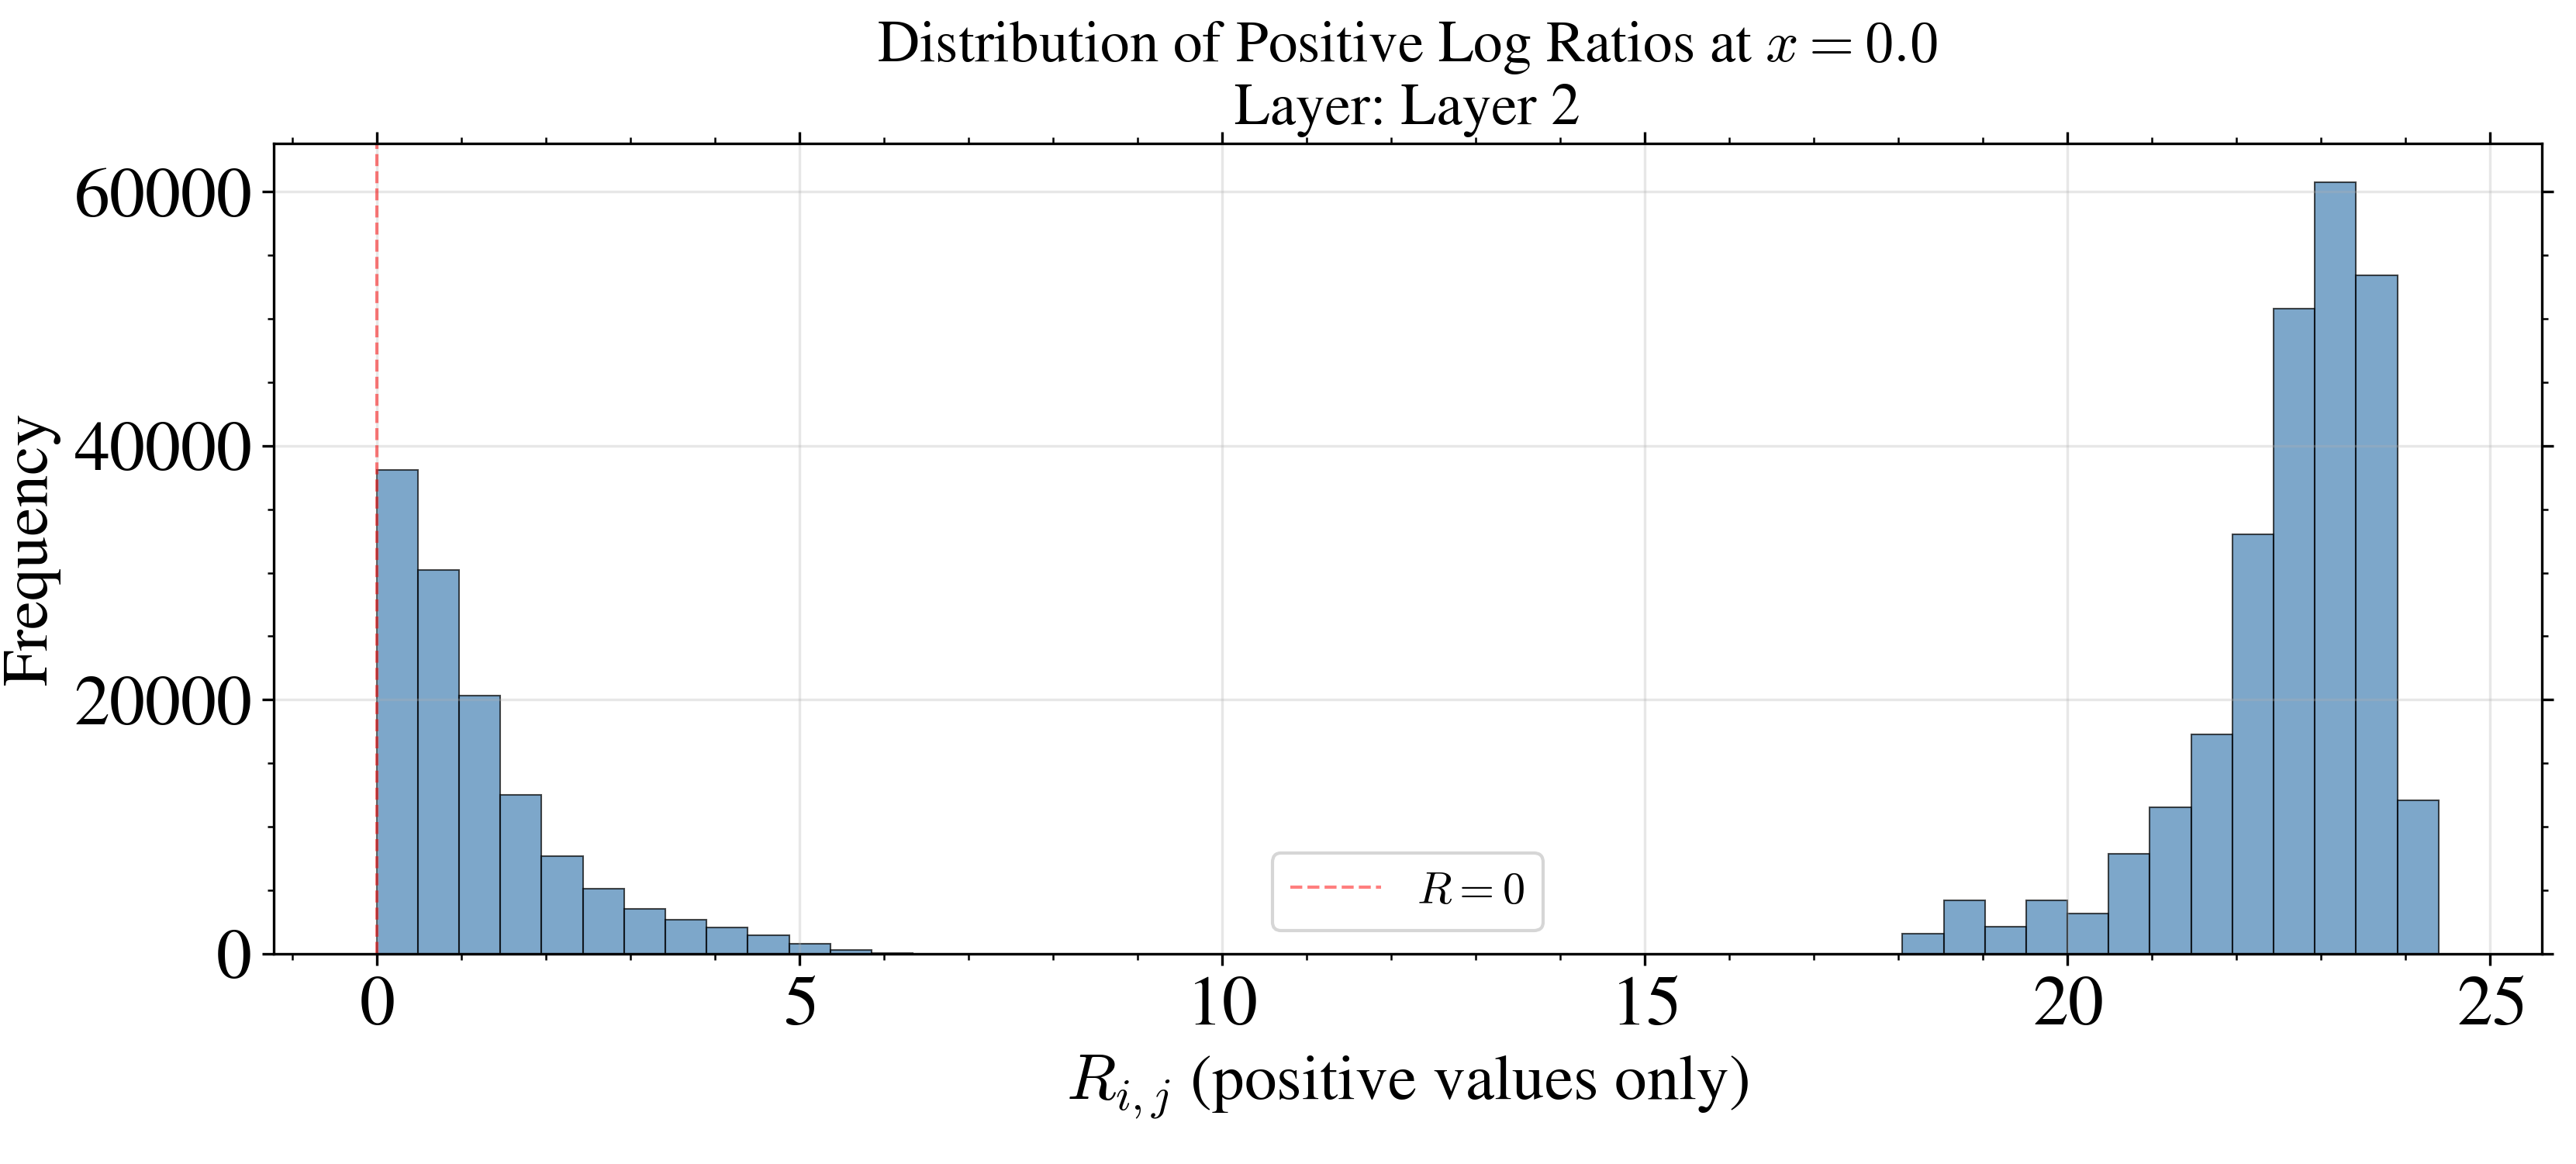
\includegraphics[width=\linewidth,height=0.27\textheight,keepaspectratio]{logratio_statistics_x0.png}
    \end{column}
    \begin{column}{0.49\textwidth}
      
\includegraphics[width=\linewidth,height=0.27\textheight,keepaspectratio]{final_prediction.png}
    \end{column}
  \end{columns}
  \vspace{0.4em}
  \begin{columns}[T]
    \begin{column}{0.49\textwidth}
      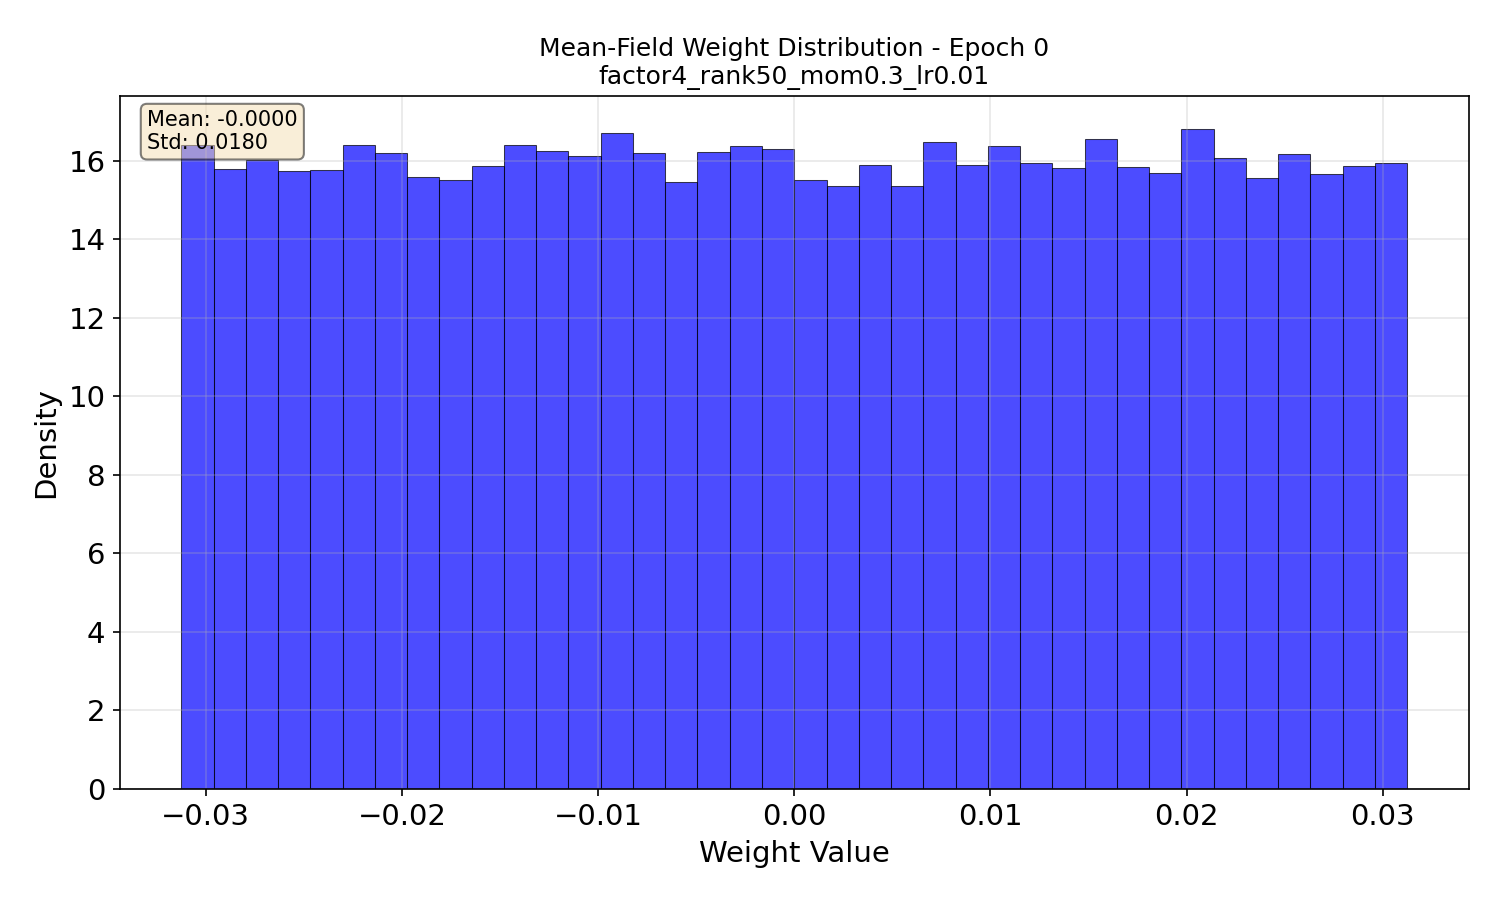
\includegraphics[width=\linewidth,height=0.27\textheight,keepaspectratio]{meanfield_density_epoch0.png}
    \end{column}
    \begin{column}{0.49\textwidth}
      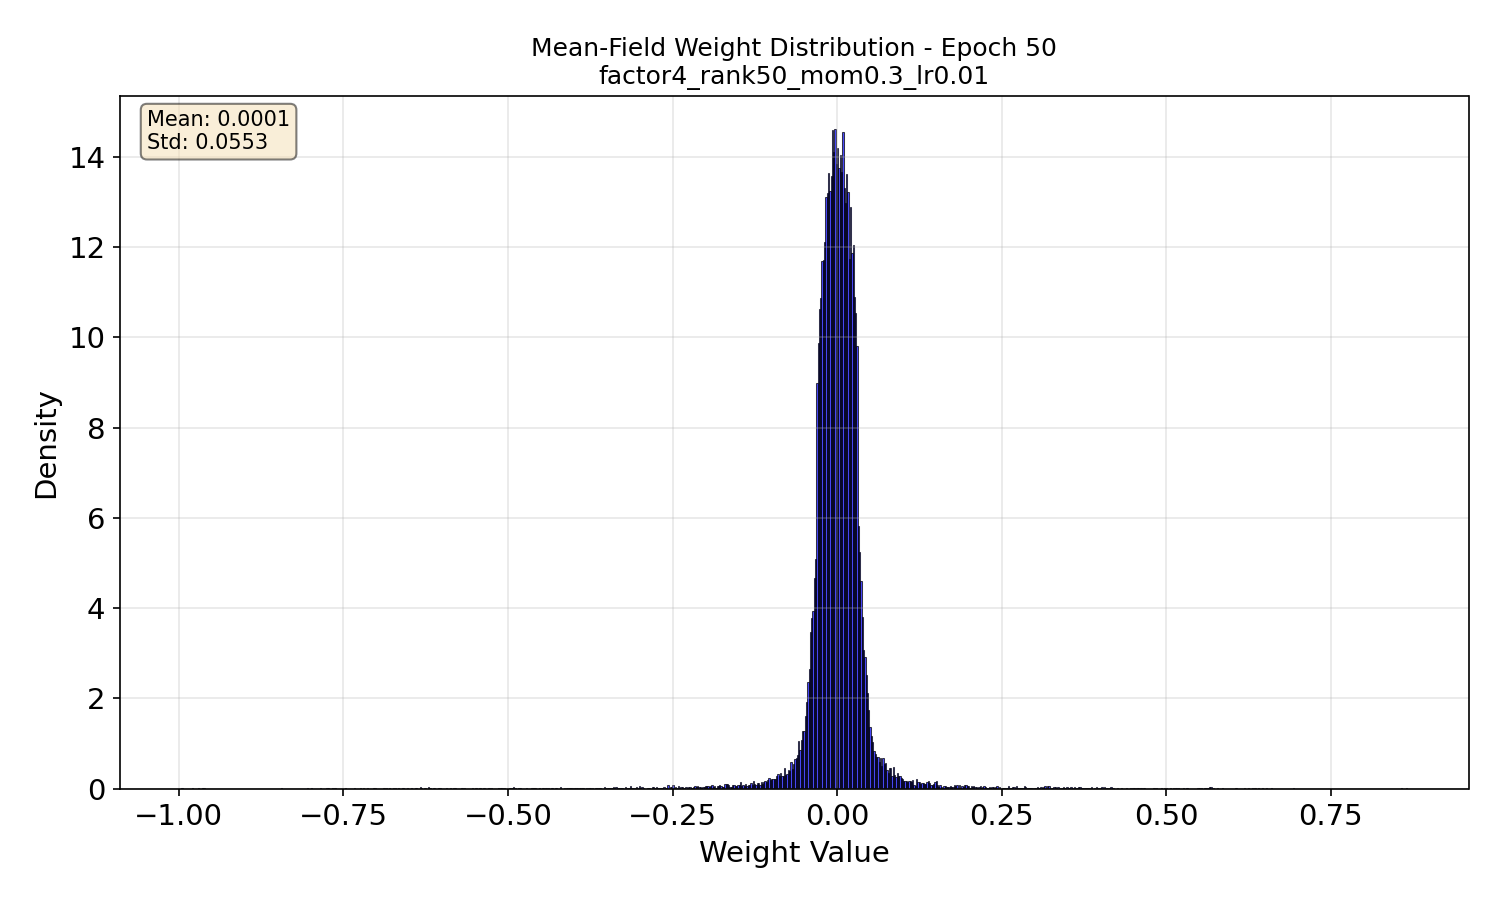
\includegraphics[width=\linewidth,height=0.27\textheight,keepaspectratio]{meanfield_density_epoch50.png}
    \end{column}
  \end{columns}
\end{frame}

\begin{frame}{Appendix: NTK Background Gallery}
  \begin{columns}[T]
    \begin{column}{0.49\textwidth}
      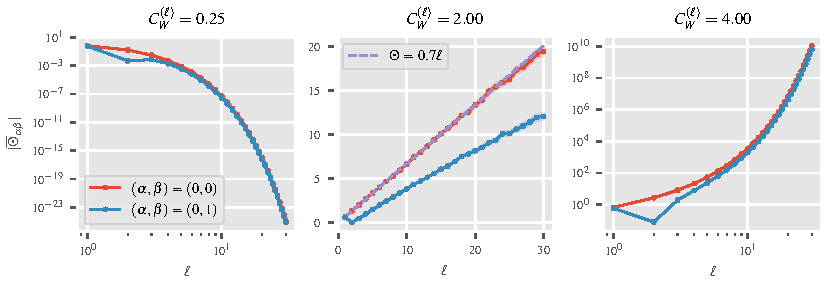
\includegraphics[width=\linewidth,height=0.31\textheight,keepaspectratio]{ntk_comparison.pdf}
    \end{column}
    \begin{column}{0.49\textwidth}
      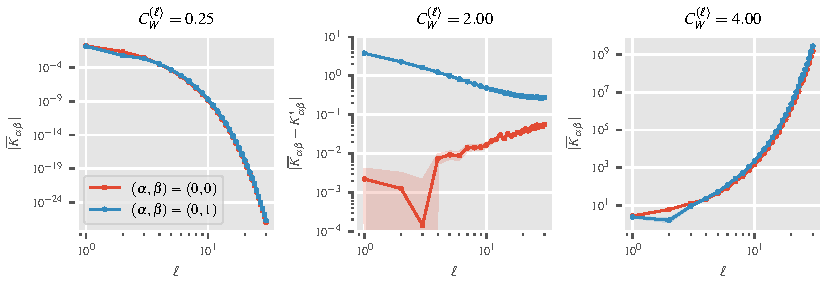
\includegraphics[width=\linewidth,height=0.31\textheight,keepaspectratio]{nngp_comparison.pdf}
    \end{column}
  \end{columns}
  \vspace{0.4em}
  \begin{center}
    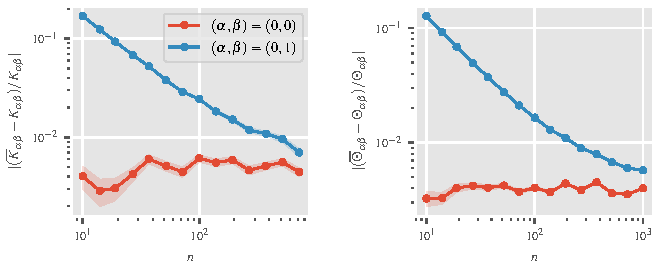
\includegraphics[width=0.58\linewidth,height=0.28\textheight,keepaspectratio]{Relu_width_corrections_layer-4.pdf}
  \end{center}
\end{frame}

\end{document}
